\begin{appendices}

\chapter{Author Contributions}
The LHC and the ATLAS experiment are projects of tremendous scale. Much of this dissertation covers the combined effort of thousands of contributors over the past twenty years. My own work is concentrated in chapters~\ref{ch:luminosity}, \ref{ch:backgrounds}, \ref{ch:model-independent-trilepton-search}, and \ref{ch:trilepton-resonance-search}. I was initially involved in the luminosity measurement effort, with a focus on methods using vertices reconstructed using inner detector data. After using vertices at high $z$ to constrain the presence of satellite bunches, protons in the beams outside the nominal RF buckets, I developed a luminosity measurement method using vertex counting (section~\ref{sec:luminosity-vertex}). Much of this effort involved understanding the effect of pileup on the reconstruction efficiency. Vertex counting has proved useful for measuring the luminosity in low pileup scenarios, such as the van der Meer scans and the measurement of the total inelastic cross section with the ALFA detector. 

The latter part of my dissertation work involved two searches for new phenomena using events with three or more charged leptons. The Standard Model backgrounds are sufficiently small that backgrounds from non-prompt sources, such as misidentified jets or semileptonic heavy flavor decays, can make significant contributions. I provided the data-driven estimate of the non-prompt electron backgrounds in the context of the model-independent trilepton search (section~\ref{sec:electron-fake-factors}). Starting from the model-independent search's framework, I then helped to develop the trilepton resonance search. I contributed to most aspects of the analysis, including the event selection, the signal and control region definitions, the non-prompt background estimation, the systematic uncertainties, and the parametrization of the background using the analytical fit functions.

\chapter{Trilepton Resonance Search}\label{sec:appendix-resonance}

\subsection{Signal Fit Details}\label{sec:appendix-resonance-signal-fits}
Tables \ref{table:ZeFitParamsSS}-\ref{table:ZmuFitParamsVLL} show the results of fitting the Voigtian plus Landau function to each signal point for the type~III seesaw and vector-like leptons models. The fits are performed in the inclusive category in $Z+e$ and $Z+\mu$ flavor channels.  


\begin{table}[h]
 \centering
\scriptsize
 \begin{tabular}{|c||c|c|c|c|c|c|}  
 \hline\hline
Mass [GeV] & $m_V$ [GeV] &  $\gamma_V$ [GeV] &  $\sigma_V$ [GeV] & $m_L$  [GeV] & $\sigma_L$ [GeV] & Ratio\\
\hline \hline
$100 $&$ 8.7222   \pm0.015 $&$ 0.131 \pm0.04 $&$ 0.32\pm0.03 $&$ 36.1\pm0.7 $&$ 10.9\pm0.355118 $&$ 0.34$ \\ 
$120 $&$ 28.5035 \pm0.024 $&$ 0.594\pm0.12 $&$ 0.72\pm0.06 $&$ 34.1\pm0.8 $&$ 10.2\pm0.391391 $&$ 0.59$ \\
$160 $&$ 68.3224 \pm0.037 $&$ 1.34\pm0.15 $&$ 1.13\pm0.08 $&$ 45.9\pm0.7 $&$ 15.3\pm0.392333 $&$ 0.57 $\\
$200 $&$ 108.294 \pm0.052 $&$ 1.86\pm0.20 $&$ 1.59\pm0.10 $&$ 59.1\pm1.1 $&$ 21.3\pm0.568737 $&$ 0.58 $\\
$250 $&$ 158.039 \pm0.090 $&$ 3.08\pm0.37 $&$ 1.48\pm0.26 $&$ 75.6\pm2.1 $&$ 27.6\pm1.10452 $&$ 0.59$ \\ 
$300 $&$ 207.856 \pm0.129 $&$ 2.96\pm0.45 $&$ 2.75\pm0.23 $&$ 92.3\pm2.6 $&$ 35.7\pm1.39974 $&$ 0.55 $\\ 
$350 $&$ 257.775\pm0.169 $&$ 4.52\pm0.63 $&$ 3.21\pm0.33 $&$ 106.8\pm3.4 $&$ 41.6\pm1.85383 $&$ 0.57$ \\ 
$400 $&$ 308.066\pm0.198 $&$ 6.84\pm0.77 $&$ 2.77\pm0.48 $&$ 129.7\pm4.2 $&$ 51.3\pm2.34715 $&$ 0.55 $\\ 
$450 $&$ 357.463\pm0.277 $&$ 7.37\pm1.05 $&$ 3.91\pm0.61 $&$ 142.1\pm5.3 $&$ 58.3\pm3.06396 $&$ 0.54$ \\ 
$500 $&$ 407.731\pm0.262 $&$ 5.39\pm1.02 $&$ 5.26\pm0.53 $&$ 179.9\pm6.1 $&$ 71.5\pm3.65063   $&$ 0.52 $ \\
\hline\hline
\end{tabular} 
\caption{Fit parameters for the type~III seesaw model in the $Z+e$ flavor channel and inclusive category. $m_V$, $\gamma_V$, and $\sigma_V$ represent the mean, Lorentzian width, and Gaussian width of the Voigt function, and $m_L$ and $\sigma_L$ represent the mean and width of the Landau function. Note that the absence of the intrinsic width of the $Z$ boson in the simulation leads to smaller values than expected for the width of the Voigtian peak for masses below $\sim250 \GeV$.}

   \label{table:ZeFitParamsSS}
\end{table}


\begin{table}[h]
 \centering
\scriptsize
 \begin{tabular}{|c||c|c|c|c|c|c|}  
 \hline\hline
Mass [GeV] & $m_V$ [GeV] &  $\gamma_V$ [GeV] &  $\sigma_V$ [GeV] & $m_L$  [GeV] & $\sigma_L$ [GeV] & Ratio\\
\hline \hline
$100$&$8.78\pm0.01 $&$ 0.1\pm0.0$&$ 0.176\pm0.01 $&$ 35.6\pm0.5 $&$ 10.6\pm0.3 $&$0.45 $\\ 
$120$&$28.71\pm0.01 $&$ 0.28\pm0.057 $&$ 0.62\pm0.02 $&$ 31.2\pm0.5 $&$ 8.7\pm0.2 $&$0.60 $\\ 
$160$&$68.56\pm0.03 $&$ 1.86\pm0.14$&$ 1.18\pm0.08 $&$ 44.7\pm0.6 $&$ 15.3\pm0.3 $&$0.60 $\\ 
$200$&$108.3\pm0.05 $&$ 3.10\pm0.25 $&$ 1.99\pm0.13 $&$ 56.6\pm0.9 $&$ 19.4\pm0.5 $&$0.61$\\ 
$250$&$158.1\pm0.1 $&$ 4.36\pm0.61 $&$ 3.64\pm0.31 $&$ 73.6\pm1.9 $&$ 27.0\pm1.0 $&$0.61 $\\ 
$300$&$207.7\pm0.1 $&$ 8.17\pm0.84 $&$ 3.87\pm0.46 $&$ 86.2\pm2.4 $&$ 32.3\pm1.3 $&$0.61$ \\ 
$350$&$258.3\pm0.2 $&$ 10.04\pm1.44 $&$ 6.15\pm0.75 $&$ 103.1\pm3.2 $&$ 40.2\pm1.7 $&$0.59 $\\ 
$400$&$307.2\pm0.3 $&$ 13.09\pm1.69 $&$ 6.39\pm0.98 $&$ 120.9\pm4.2 $&$ 50.2\pm2.3 $&$0.58$ \\ 
$450$&$357.4\pm0.5 $&$ 18.08\pm3.05 $&$ 8.86\pm1.64 $&$ 137.7\pm5.9 $&$ 57.9\pm3.4 $&$0.56$ \\ 
$500$&$407.6\pm0.5 $&$ 14.20\pm3.10 $&$ 12.2\pm1.44 $&$ 166.7\pm6.1 $&$ 67.9\pm3.6 $&$0.53 $\\ 
\hline\hline
\end{tabular} 
\caption{Fit parameters for the type~III seesaw model in the $Z+\mu$ flavor channel and inclusive category. $m_V$, $\gamma_V$, and $\sigma_V$ represent the mean, Lorentzian width, and Gaussian width of the Voigt function, and $m_L$ and $\sigma_L$ represent the mean and width of the Landau function. Note that the absence of the intrinsic width of the $Z$ boson in the simulation leads to smaller values than expected for the width of the Voigtian peak for masses below $\sim250 \GeV$.}
   \label{table:ZmuFitParamsSS}
\end{table}


\begin{table}[h]
 \centering
\scriptsize
\begin{tabular}{|c||c|c|c|c|c|c|} 
\hline\hline
Mass [GeV] & $m_V$ [GeV] &  $\gamma_V$ [GeV] &  $\sigma_V$ [GeV] & $m_L$  [GeV] & $\sigma_L$ [GeV] & Ratio\\
\hline \hline
$100$&$10.77\pm0.18 $&$ 0.1\pm0.1 $&$ 2.5\pm0.2 $&$ 34.3\pm1.5 $&$ 12.12\pm0.47$&$0.37$\\ 
$110$&$18.54\pm0.04 $&$ 1.9\pm0.2 $&$ 1.0\pm0.1 $&$ 34.1\pm1.8 $&$ 10.08\pm0.51$&$0.69$\\ 
$120$&$28.25\pm0.04 $&$ 2.7\pm0.4 $&$ 0.7\pm0.2 $&$ 35.8\pm3.0 $&$ 10.95\pm1.02$&$0.75$ \\ 
$130$&$38.18\pm0.04 $&$ 2.2\pm0.2 $&$ 1.2\pm0.1$&$ 31.0\pm0.6 $&$ 9.40\pm0.32$&$0.71$ \\ 
$140$&$48.07\pm0.04 $&$ 2.2\pm0.2 $&$ 1.5\pm0.1 $&$ 33.4\pm0.6 $&$ 10.29\pm0.28$&$0.69$ \\ 
$160$&$68.00\pm0.04 $&$ 3.0\pm0.2 $&$ 1.4\pm0.1 $&$ 37.0\pm0.7 $&$ 11.52\pm0.32$&$0.70$ \\ 
$180$&$87.97\pm0.05 $&$ 3.2\pm0.2 $&$ 1.6\pm0.1 $&$ 43.8\pm0.7 $&$ 14.05\pm0.35$&$0.67$ \\ 
$200$&$107.89\pm0.05 $&$ 3.0\pm0.2 $&$ 2.0\pm0.1 $&$ 49.7\pm0.8 $&$ 16.38\pm0.39$&$0.65$ \\ 
$250$&$157.75\pm0.06 $&$ 3.2\pm0.2 $&$ 2.6\pm0.2 $&$ 66.2\pm0.9 $&$ 22.76\pm0.47$&$0.59$ \\ 
$300$&$207.57\pm0.07 $&$ 3.4\pm0.3 $&$ 3.3\pm0.2 $&$ 83.9\pm1.1 $&$ 29.64\pm0.58$&$0.57$ \\ 
$400$&$307.53\pm0.09 $&$ 4.2\pm0.3 $&$ 4.4\pm0.2 $&$ 118.9\pm1.7 $&$ 46.42\pm0.93$&$0.53$ \\ 
 \hline\hline
\end{tabular} 
\caption{Fit parameters for the VLL model in the $Z+e$ flavor channel and inclusive category. $m_V$, $\gamma_V$, and $\sigma_V$ represent the mean, Lorentzian width, and Gaussian width of the Voigt function, and $m_L$ and $\sigma_L$ represent the mean and width of the Landau function.}

   \label{table:ZeFitParamsVLL}
\end{table}


\begin{table}[h]
 \centering
\scriptsize
\begin{tabular}{|c||c|c|c|c|c|c|} 
 \hline\hline
Mass [GeV] & $m_V$ [GeV] &  $\gamma_V$ [GeV] &  $\sigma_V$ [GeV] & $m_L$  [GeV] & $\sigma_L$ [GeV] & Ratio\\
\hline \hline
$100$&$10.9\pm0.13 $&$ 0.1\pm0.05 $&$ 2.85\pm0.10 $&$ 35.63\pm1.21 $&$ 11.98\pm0.40$&$0.44$\\
$110$&$18.7\pm0.03$&$ 2.13\pm0.16 $&$ 0.73\pm0.11 $&$ 32.88\pm1.55 $&$ 9.47\pm0.46$&$0.74$\\
$120$&$28.5\pm0.03 $&$ 2.26\pm0.19 $&$ 0.78\pm0.11 $&$ 30.72\pm1.17 $&$ 9.44\pm0.59$&$0.75$\\
$130$&$38.4\pm0.03 $&$ 2.23\pm0.16 $&$ 1.07\pm0.09 $&$ 29.40\pm0.48 $&$ 8.83\pm0.26$&$0.73$\\
$140$&$48.5\pm0.03$&$ 2.38\pm0.16 $&$ 1.26\pm0.09 $&$ 30.57\pm0.50 $&$ 9.31\pm0.25$&$0.73$\\
$160$&$68.5\pm0.05 $&$ 2.71\pm0.19 $&$ 1.74\pm0.10 $&$ 33.97\pm0.55 $&$ 10.45\pm0.27$&$0.71$\\
$180$&$88.3\pm0.05 $&$ 2.73\pm0.21 $&$ 2.19\pm0.11 $&$ 40.06\pm0.62 $&$ 12.76\pm0.30$&$0.68$\\
$200$&$108.4\pm0.1 $&$ 3.34\pm0.26 $&$ 2.81\pm0.14 $&$ 45.44\pm0.65 $&$ 14.28\pm0.32$&$0.66$\\
$250$&$158.2\pm0.1 $&$ 4.45\pm0.34 $&$ 3.89\pm0.17 $&$ 61.10\pm0.85 $&$ 20.71\pm0.42$&$0.62$\\
$300$&$208.0\pm0.1 $&$ 6.21\pm0.48 $&$ 5.26\pm0.25 $&$ 76.50\pm1.01 $&$ 26.62\pm0.51$&$0.58$\\
$400$&$307.9\pm0.2 $&$ 9.12\pm0.84 $&$ 8.63\pm0.40 $&$ 114.84\pm1.60 $&$ 42.99\pm0.85$&$0.53$\\
\hline\hline
\end{tabular} 
\caption{Fit parameters for the VLL model in the $Z+\mu$ flavor channel and inclusive category. $m_V$, $\gamma_V$, and $\sigma_V$ represent the mean, Lorentzian width, and Gaussian width of the Voigt function, and $m_L$ and $\sigma_L$ represent the mean and width of the Landau function.}
   \label{table:ZmuFitParamsVLL}
\end{table}



\subsection{Additional Kinematic Distributions}\label{sec:appendix-resonance-SR-distributions}
This section shows the $m_{3\ell}$, $\Delta R(Z,\ \ell_3)$, $\mtw$, and $\Etmiss$ distributions in each of the signal regions (the primary distributions are shown in section~\ref{sec:resonance-results}).

\begin{figure}[h]
  \centering
  \subfloat[ $Z+e$, inclusive] {
    \resizebox{0.48\textwidth}{!}{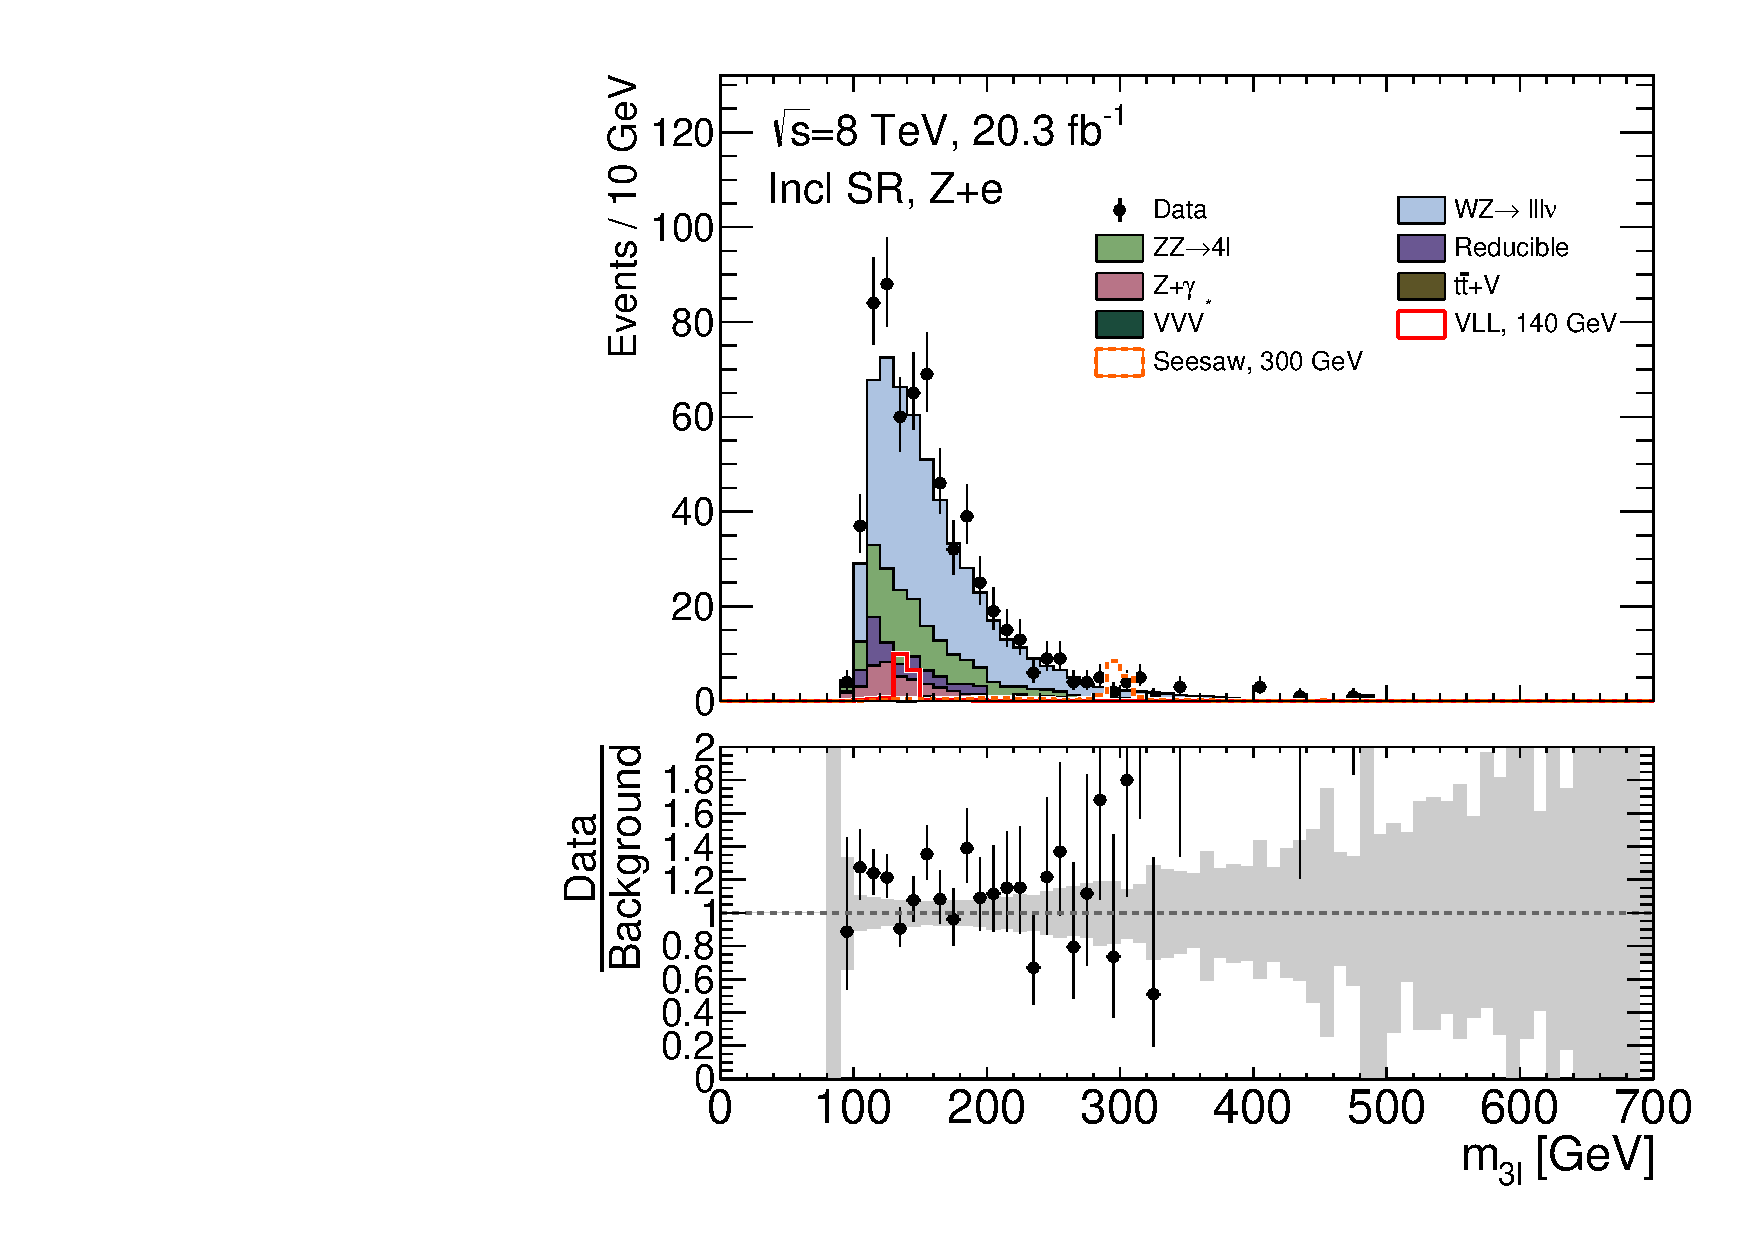
\includegraphics{figures/resonance/c_output_m3l_Ze_InclusiveNoM3L_300GeV}}
  }
  \subfloat[ $Z+\mu$, inclusive] {
    \resizebox{0.48\textwidth}{!}{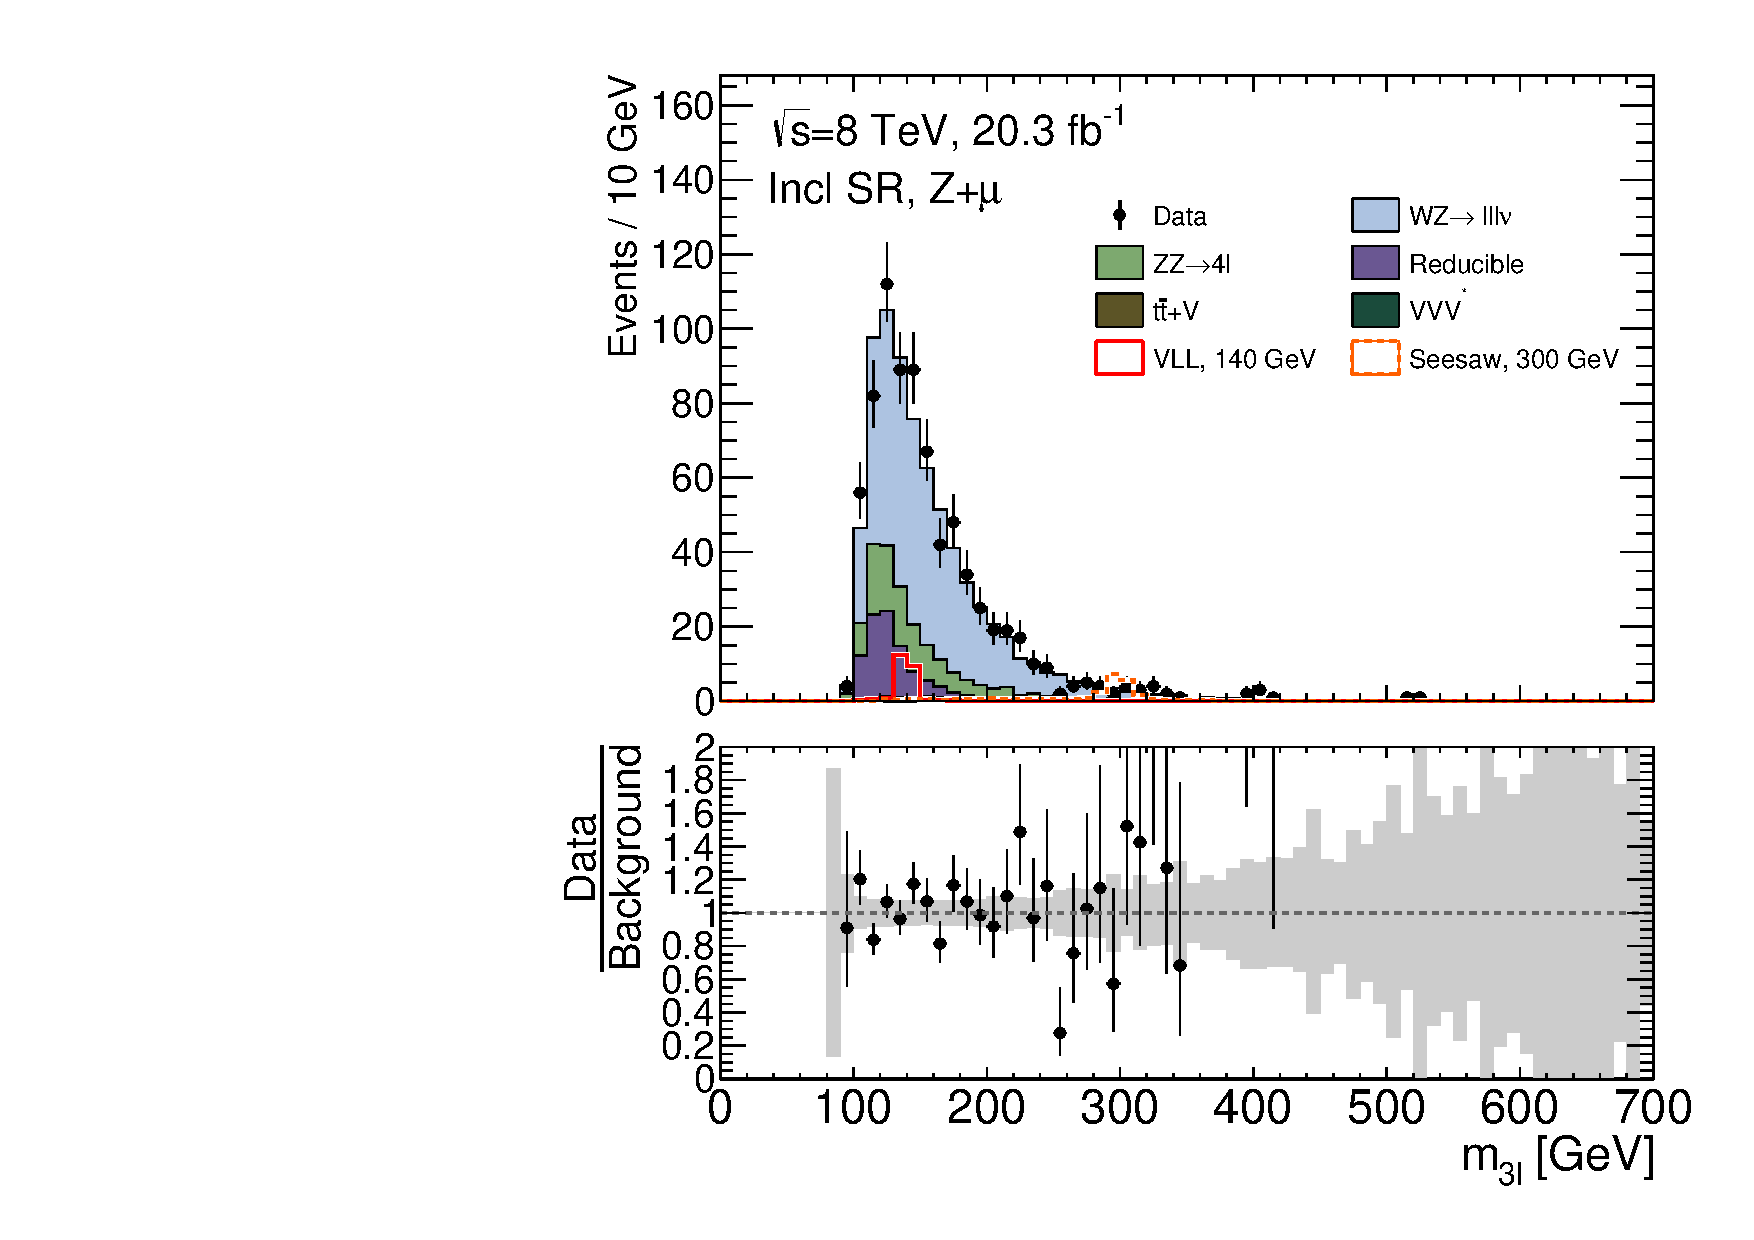
\includegraphics{figures/resonance/c_output_m3l_Zmu_InclusiveNoM3L_300GeV}}
  } \\
  \subfloat[ $Z+e$, $\fourl$ category] {
    \resizebox{0.48\textwidth}{!}{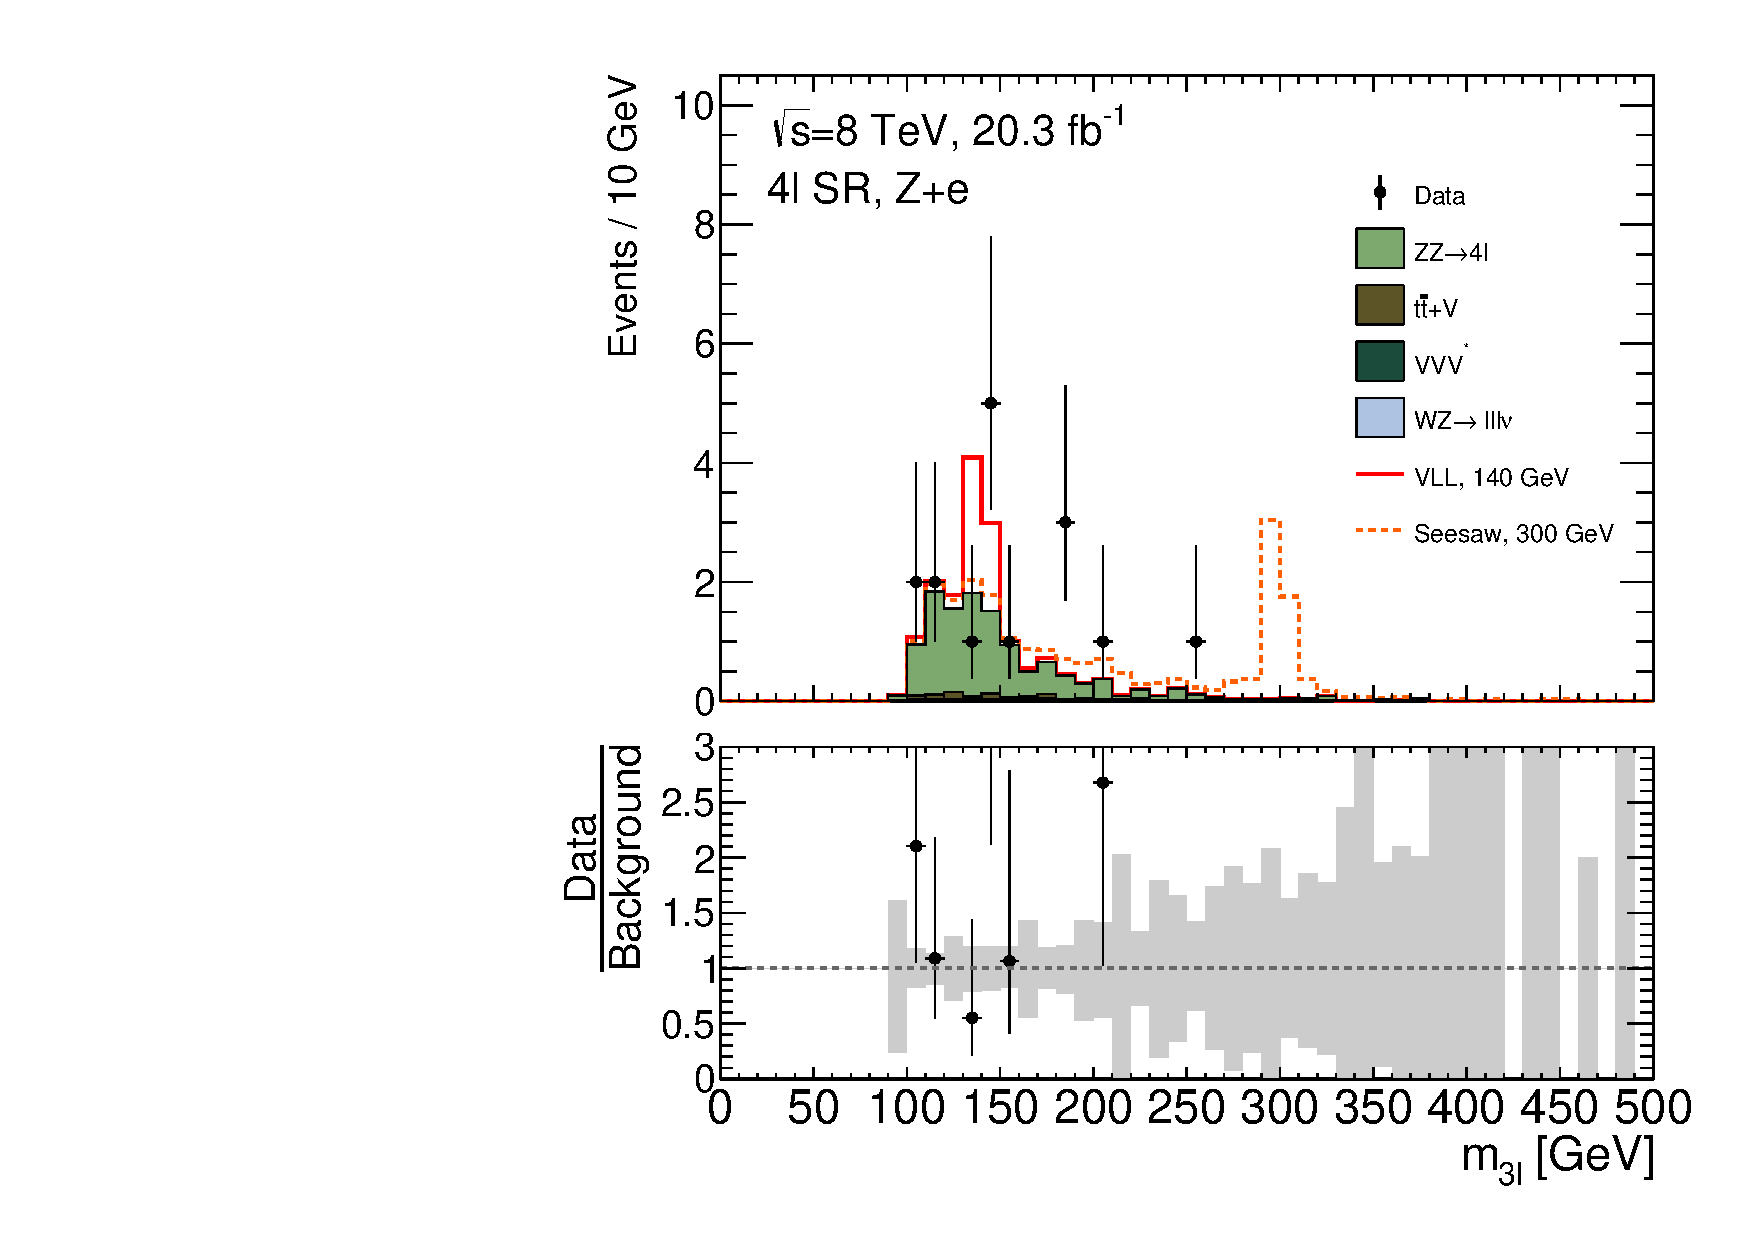
\includegraphics{figures/resonance/c_output_m3l_Ze_FourLNoM3L_300GeV}}
  }
  \subfloat[ $Z+\mu$, $\fourl$ category] {
    \resizebox{0.48\textwidth}{!}{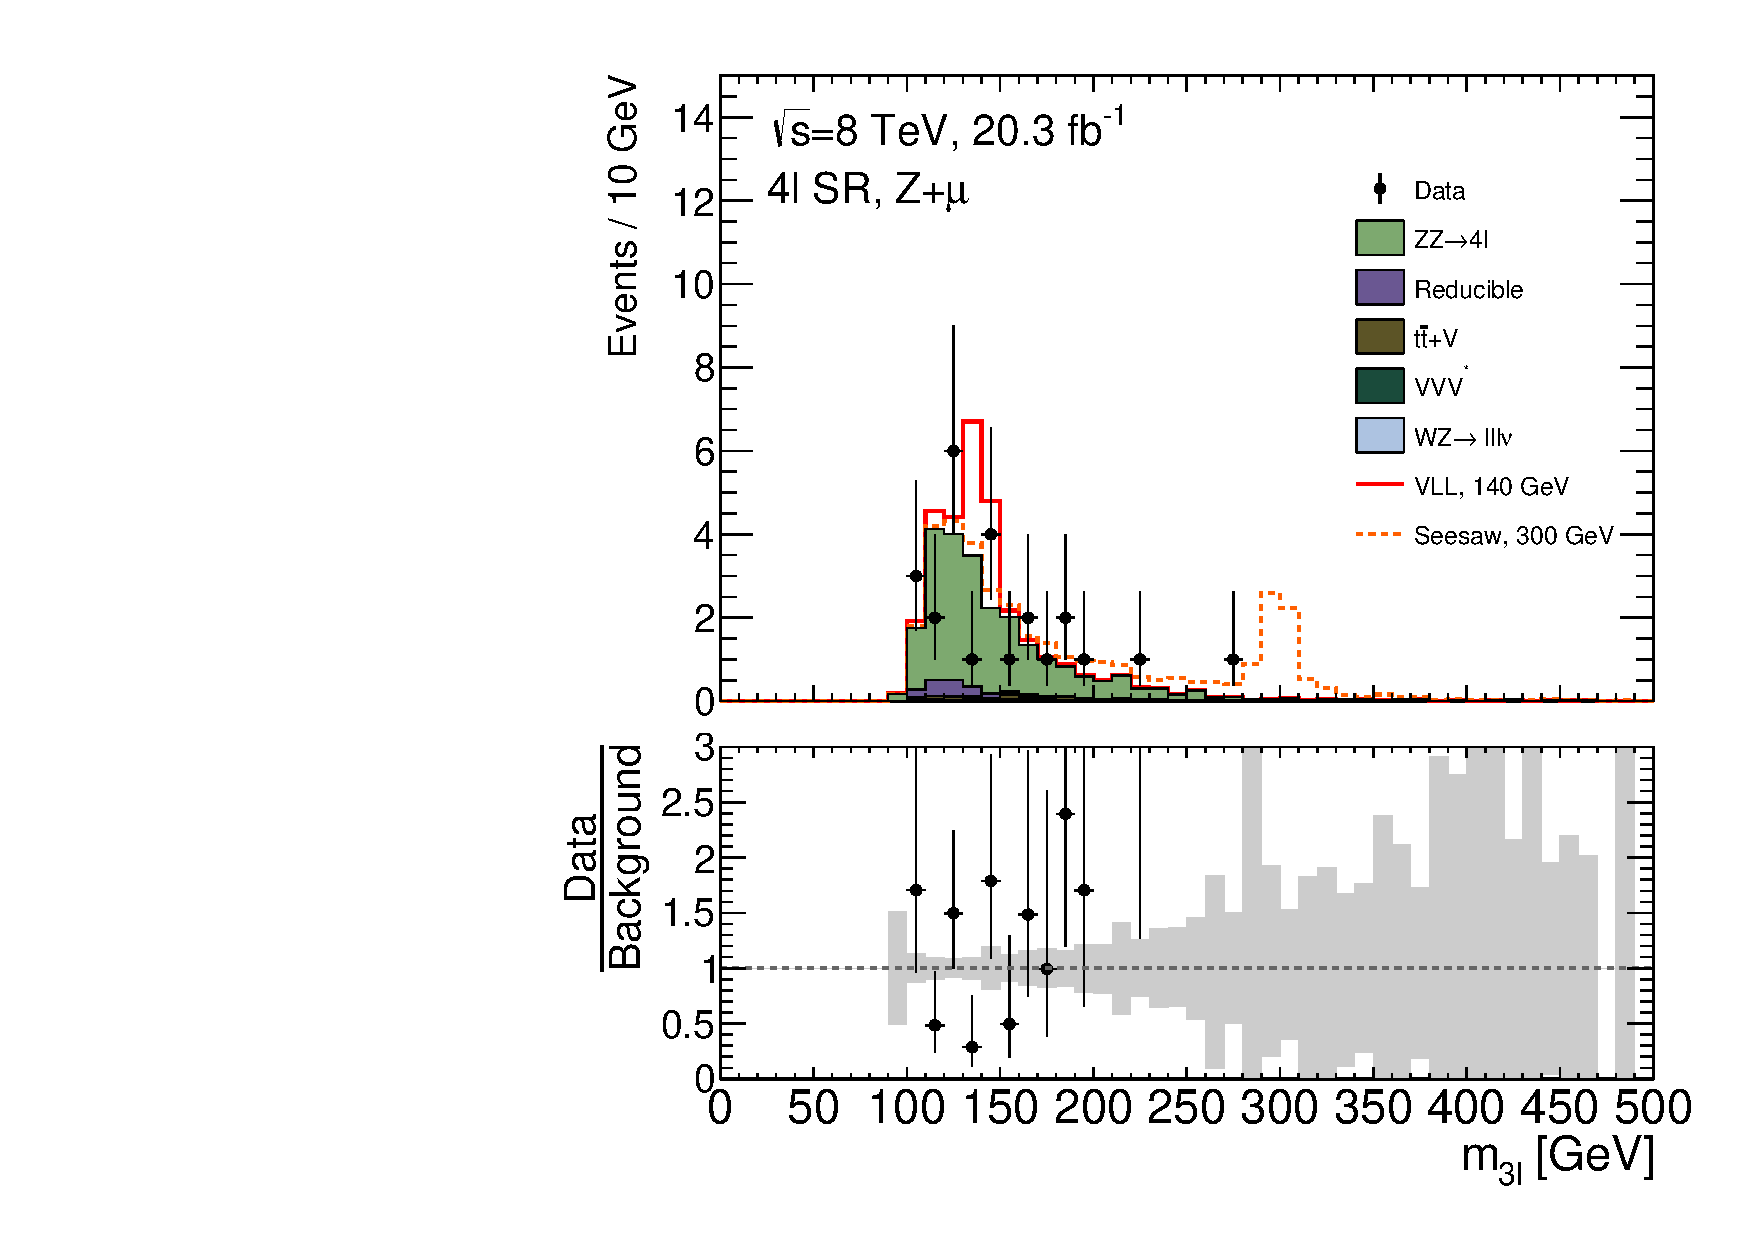
\includegraphics{figures/resonance/c_output_m3l_Zmu_FourLNoM3L_300GeV}}
  } \\
  \caption{$m_{3\ell}$ distributions for $Z+e$ and $Z+\mu$ candidates, for the inclusive and $\fourl$ signal regions (linear scale).}
  \label{fig:SR-m3l-1-linear}
\end{figure}

\begin{figure}[h]
  \centering
  \subfloat[ $Z+e$, dijet category] {
    \resizebox{0.48\textwidth}{!}{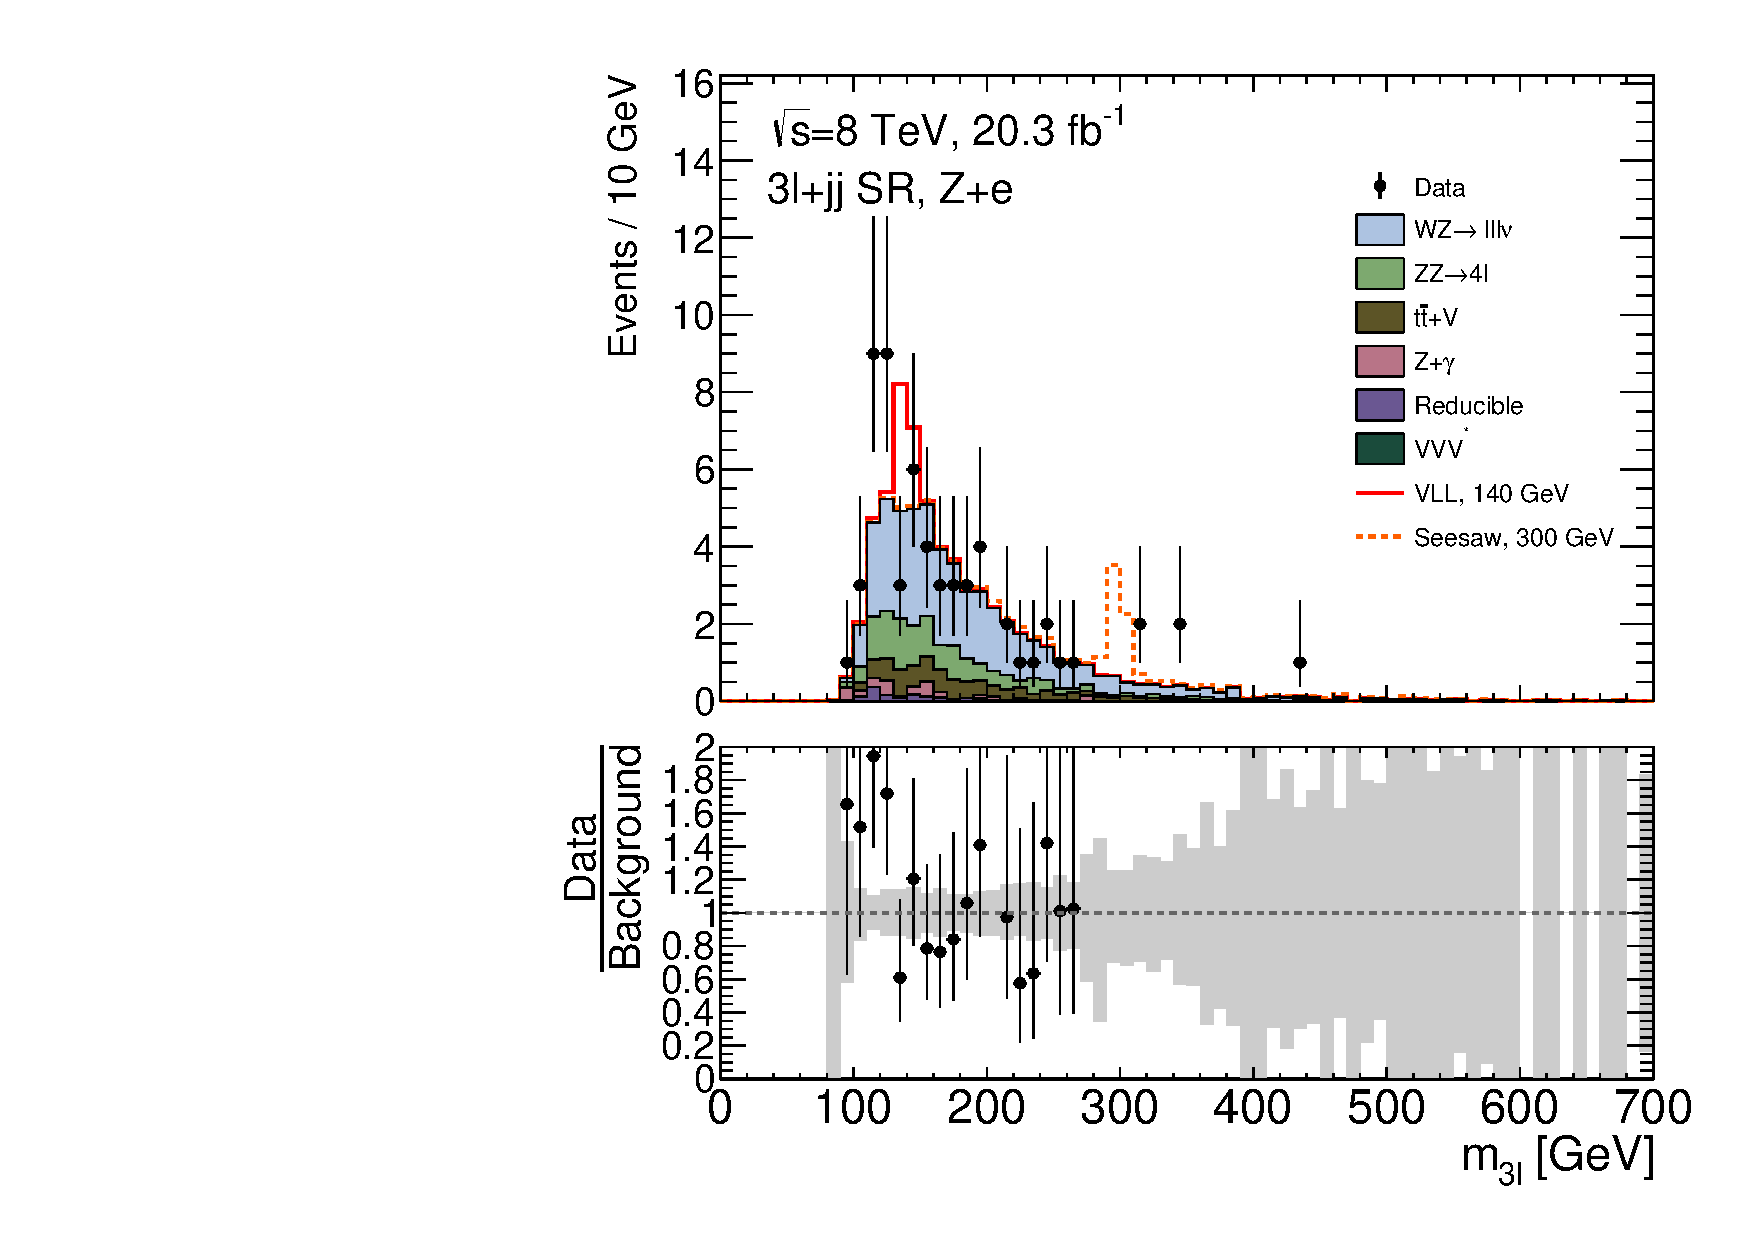
\includegraphics{figures/resonance/c_output_m3l_Ze_ThreeLDijetNoM3L_300GeV}}
  }
  \subfloat[ $Z+\mu$, dijet category] {
    \resizebox{0.48\textwidth}{!}{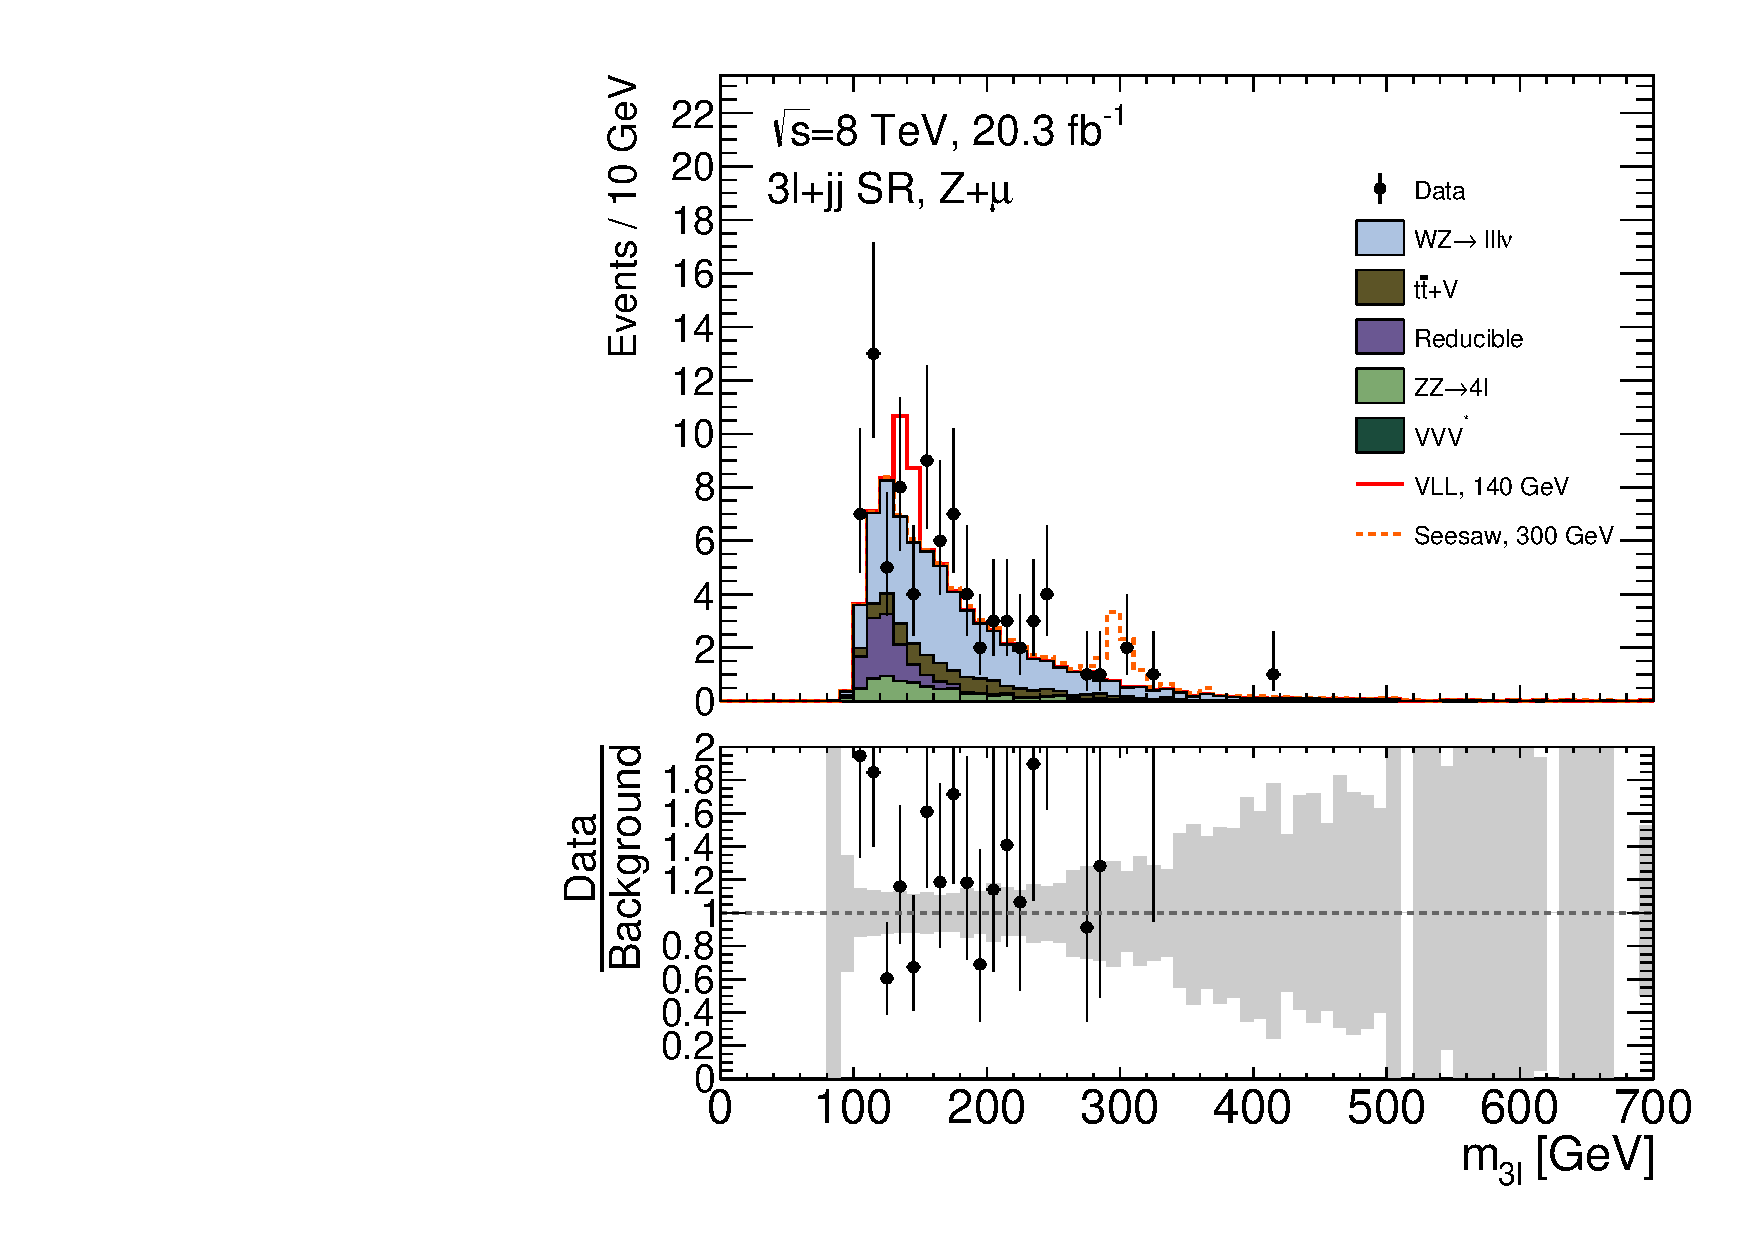
\includegraphics{figures/resonance/c_output_m3l_Zmu_ThreeLDijetNoM3L_300GeV}}
  } \\
  \subfloat[ $Z+e$, else category] {
    \resizebox{0.48\textwidth}{!}{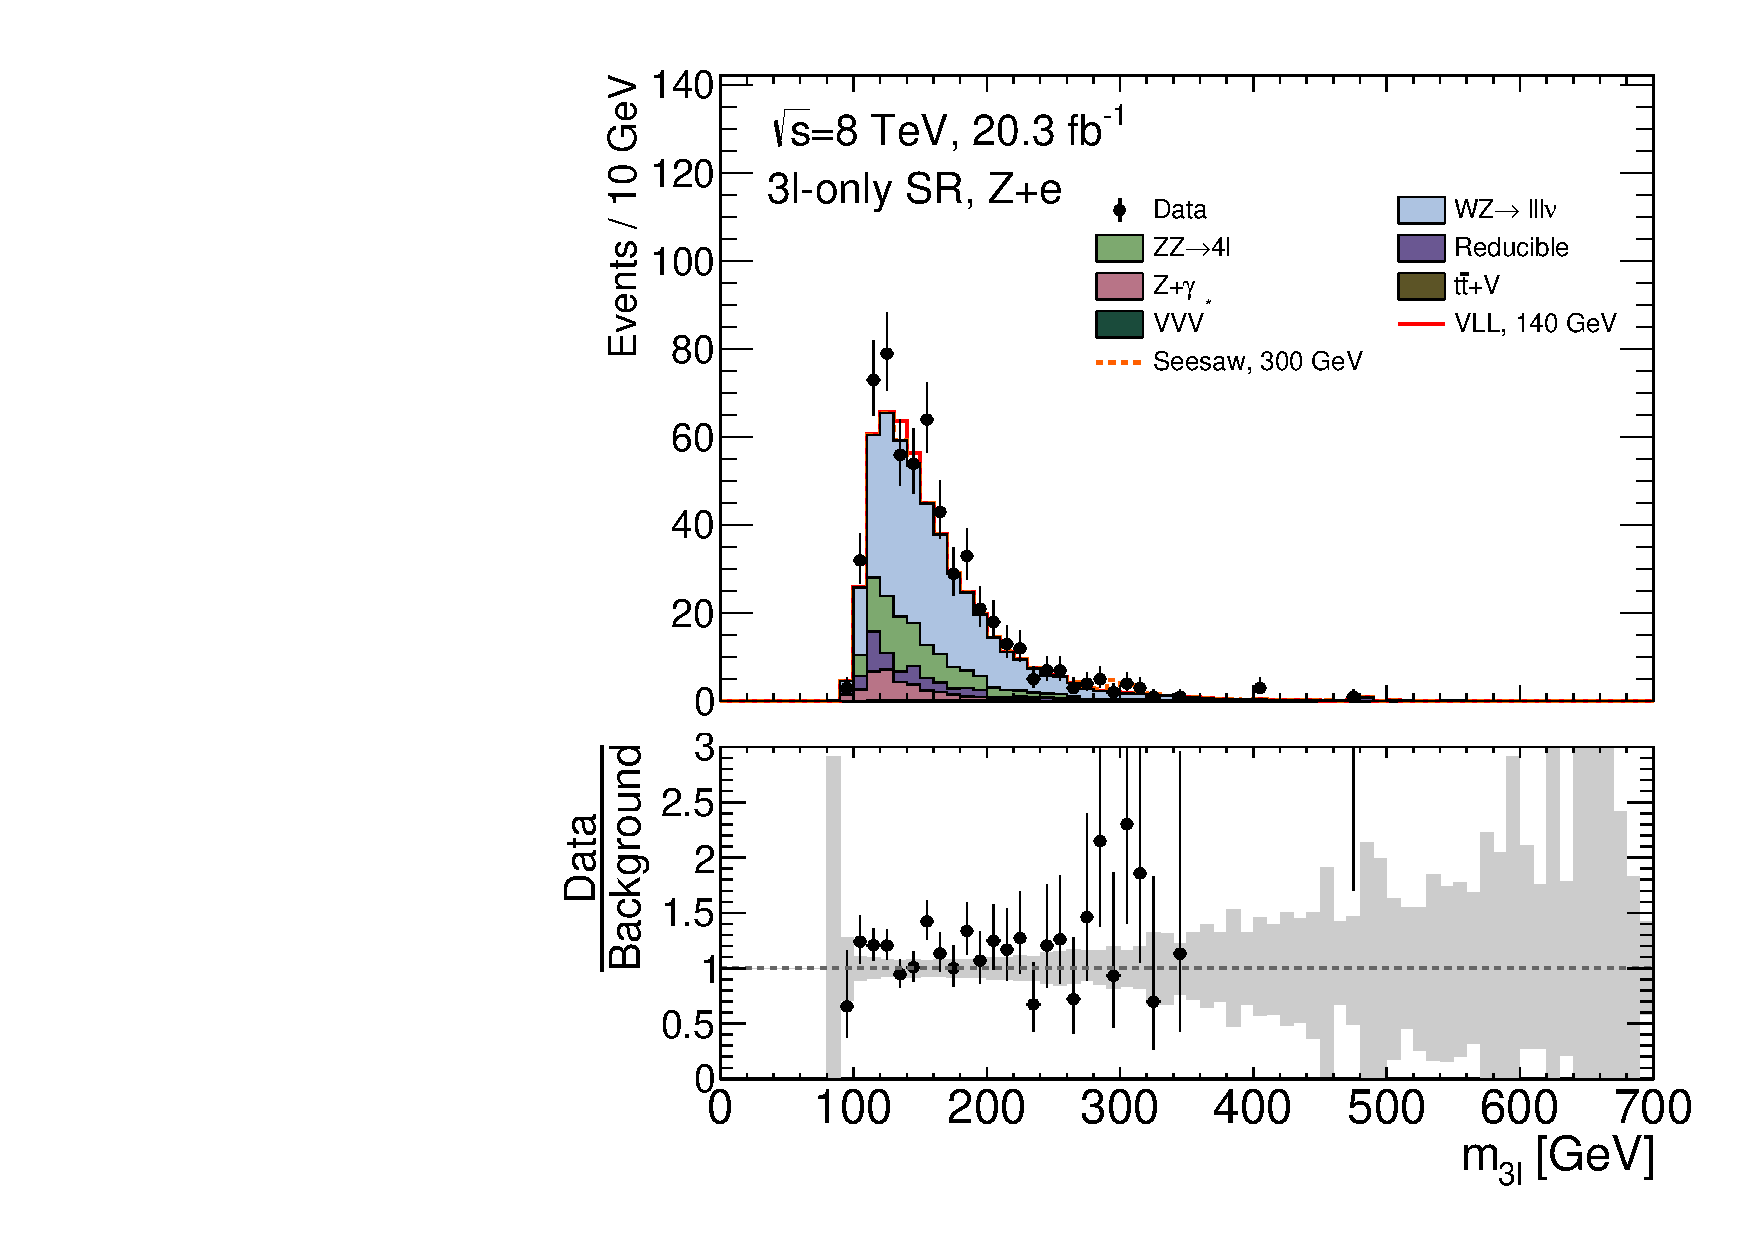
\includegraphics{figures/resonance/c_output_m3l_Ze_ElseNoM3L_300GeV}}
  }
  \subfloat[ $Z+\mu$, else category] {
    \resizebox{0.48\textwidth}{!}{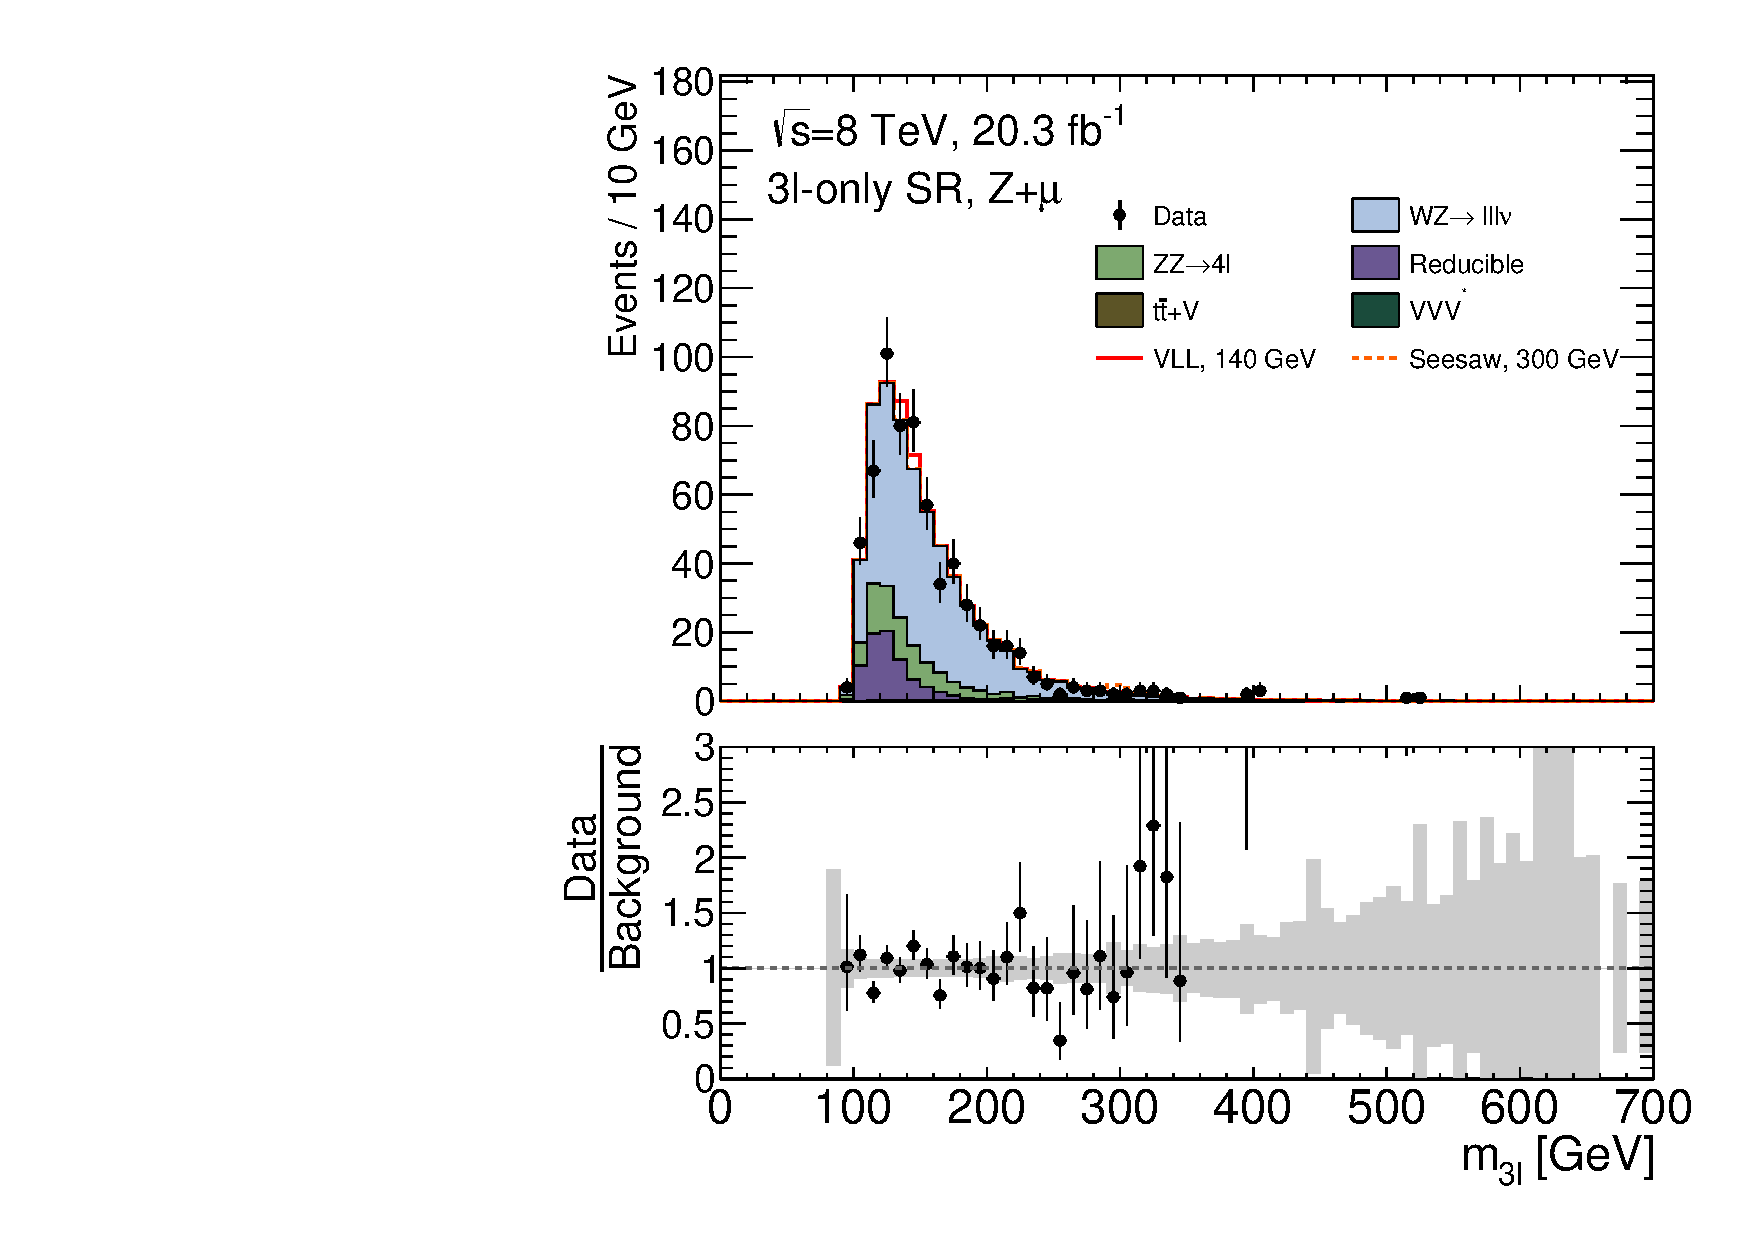
\includegraphics{figures/resonance/c_output_m3l_Zmu_ElseNoM3L_300GeV}}
  }
  \caption{$m_{3\ell}$ distributions for $Z+e$ and $Z+\mu$ candidates, for the $\threeljj$ and $\threelo$ signal regions (linear scale).}
  \label{fig:SR-m3l-2-linear}
\end{figure}


\begin{figure}[h]
  \centering
  \subfloat[ $Z+e$, inclusive] {
    \resizebox{0.48\textwidth}{!}{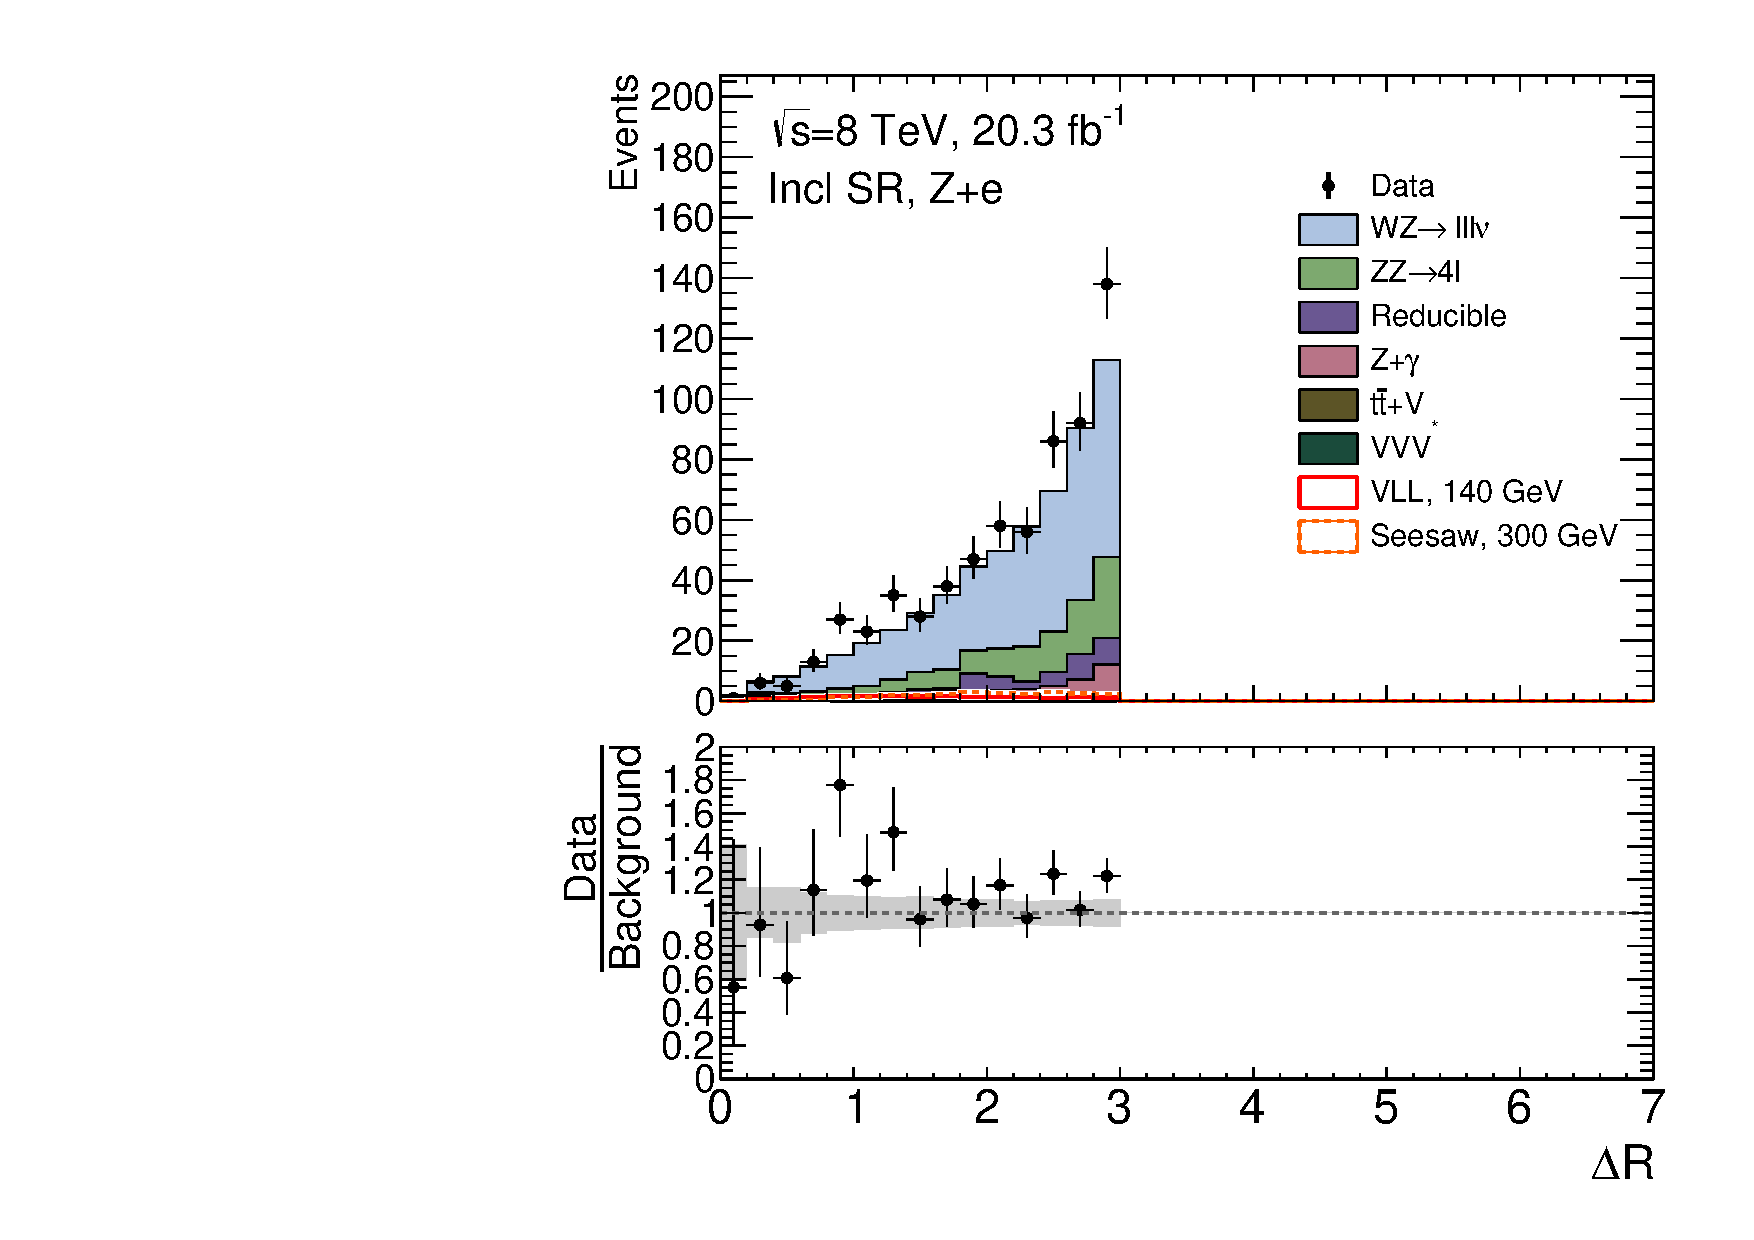
\includegraphics{figures/resonance/c_output_dR_Ze_InclusiveNoM3L_300GeV}}
  }
  \subfloat[ $Z+\mu$, inclusive] {
    \resizebox{0.48\textwidth}{!}{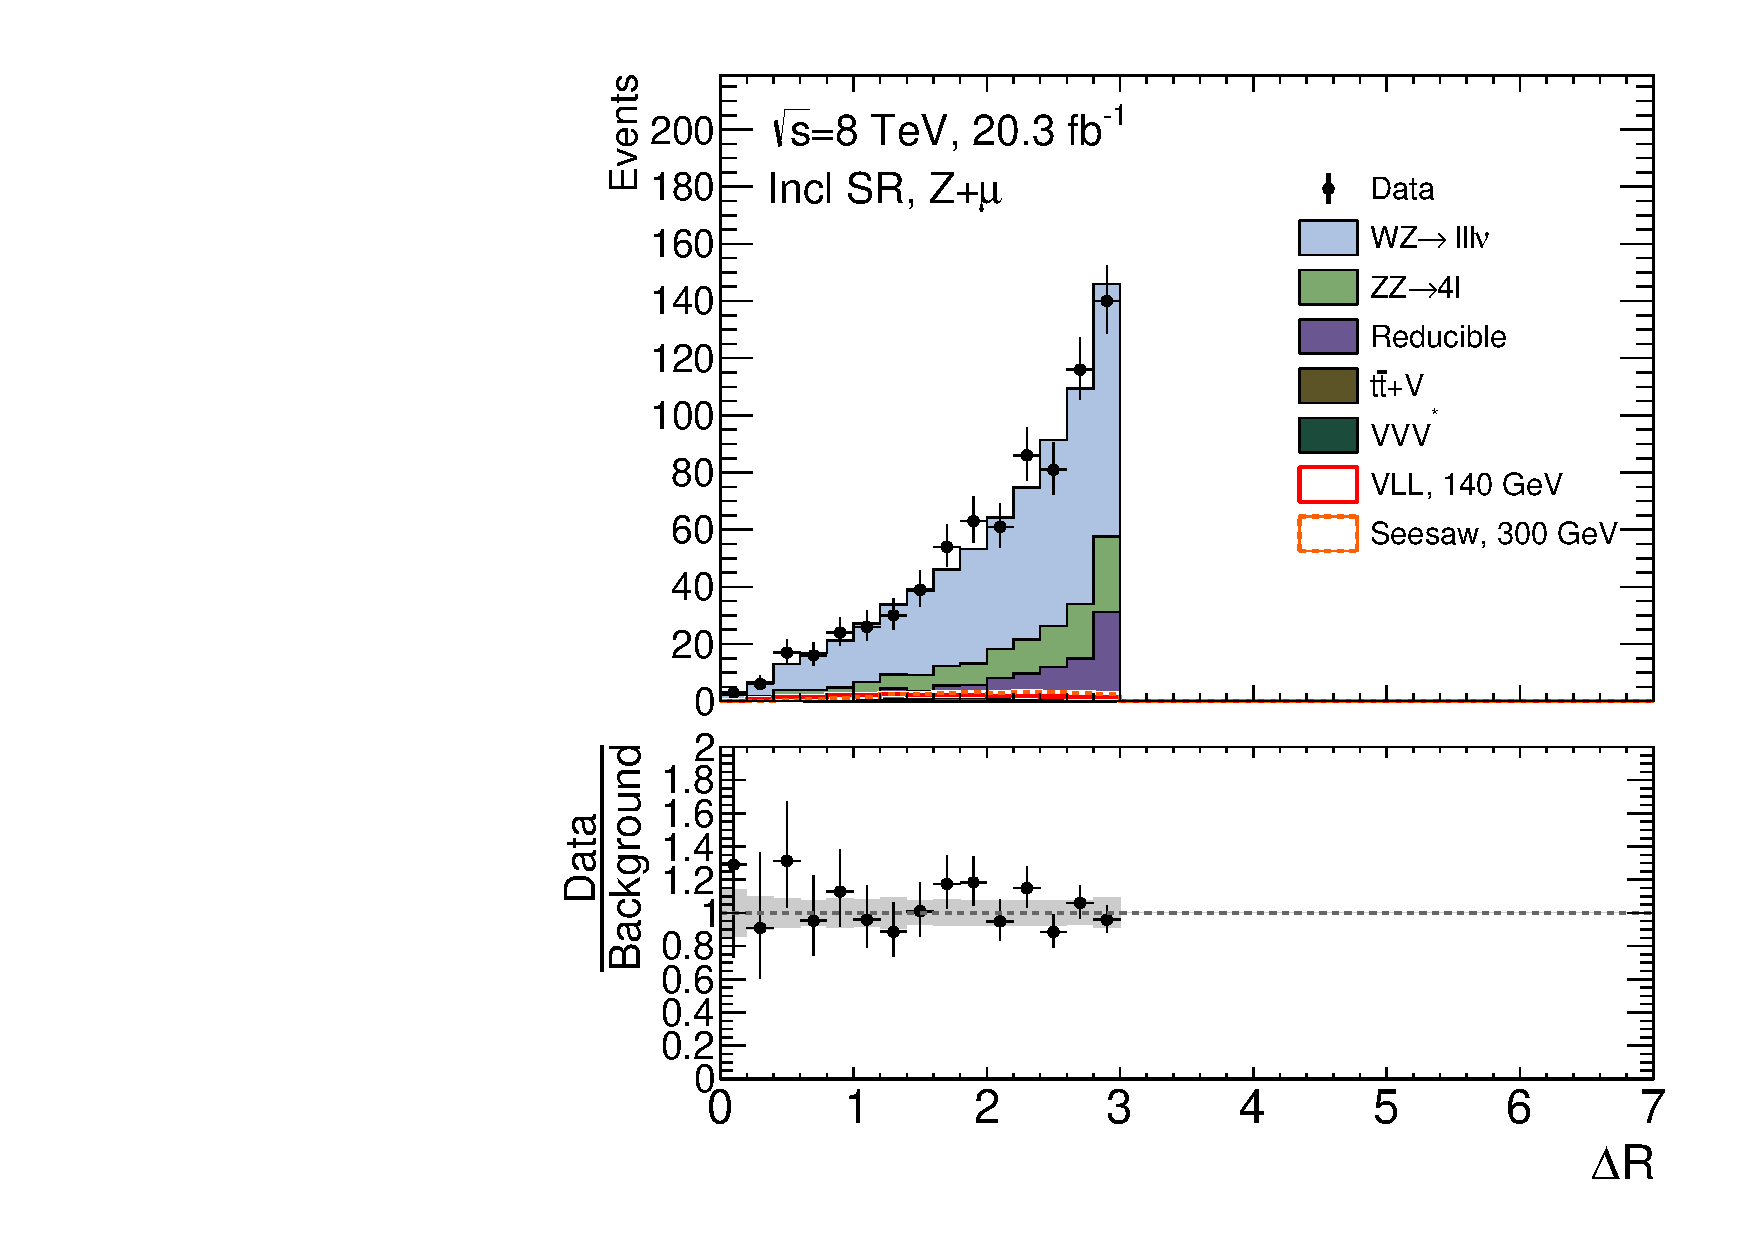
\includegraphics{figures/resonance/c_output_dR_Zmu_InclusiveNoM3L_300GeV}}
  } \\
  \subfloat[ $Z+e$, $4L$ category] {
    \resizebox{0.48\textwidth}{!}{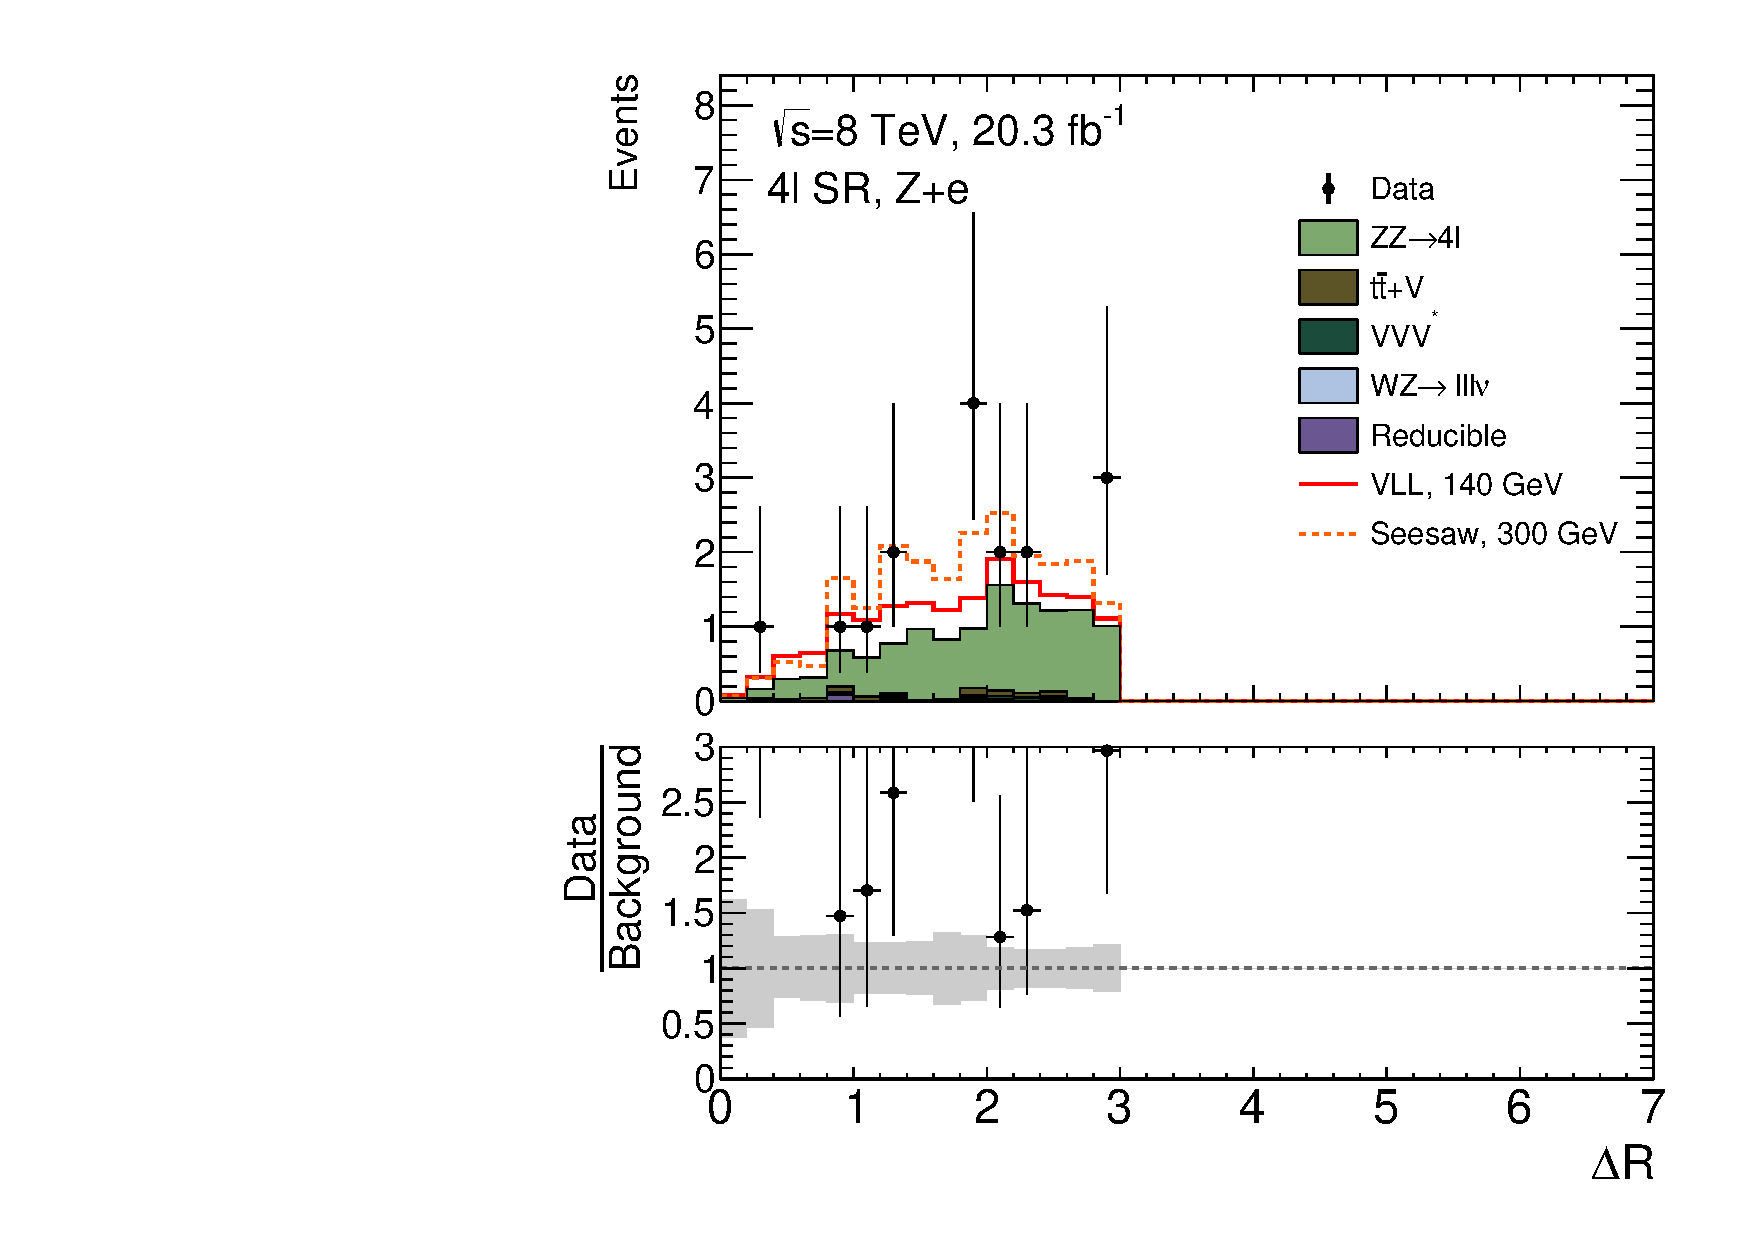
\includegraphics{figures/resonance/c_output_dR_Ze_FourLNoM3L_300GeV}}
  }
  \subfloat[ $Z+\mu$, $4L$ category] {
    \resizebox{0.48\textwidth}{!}{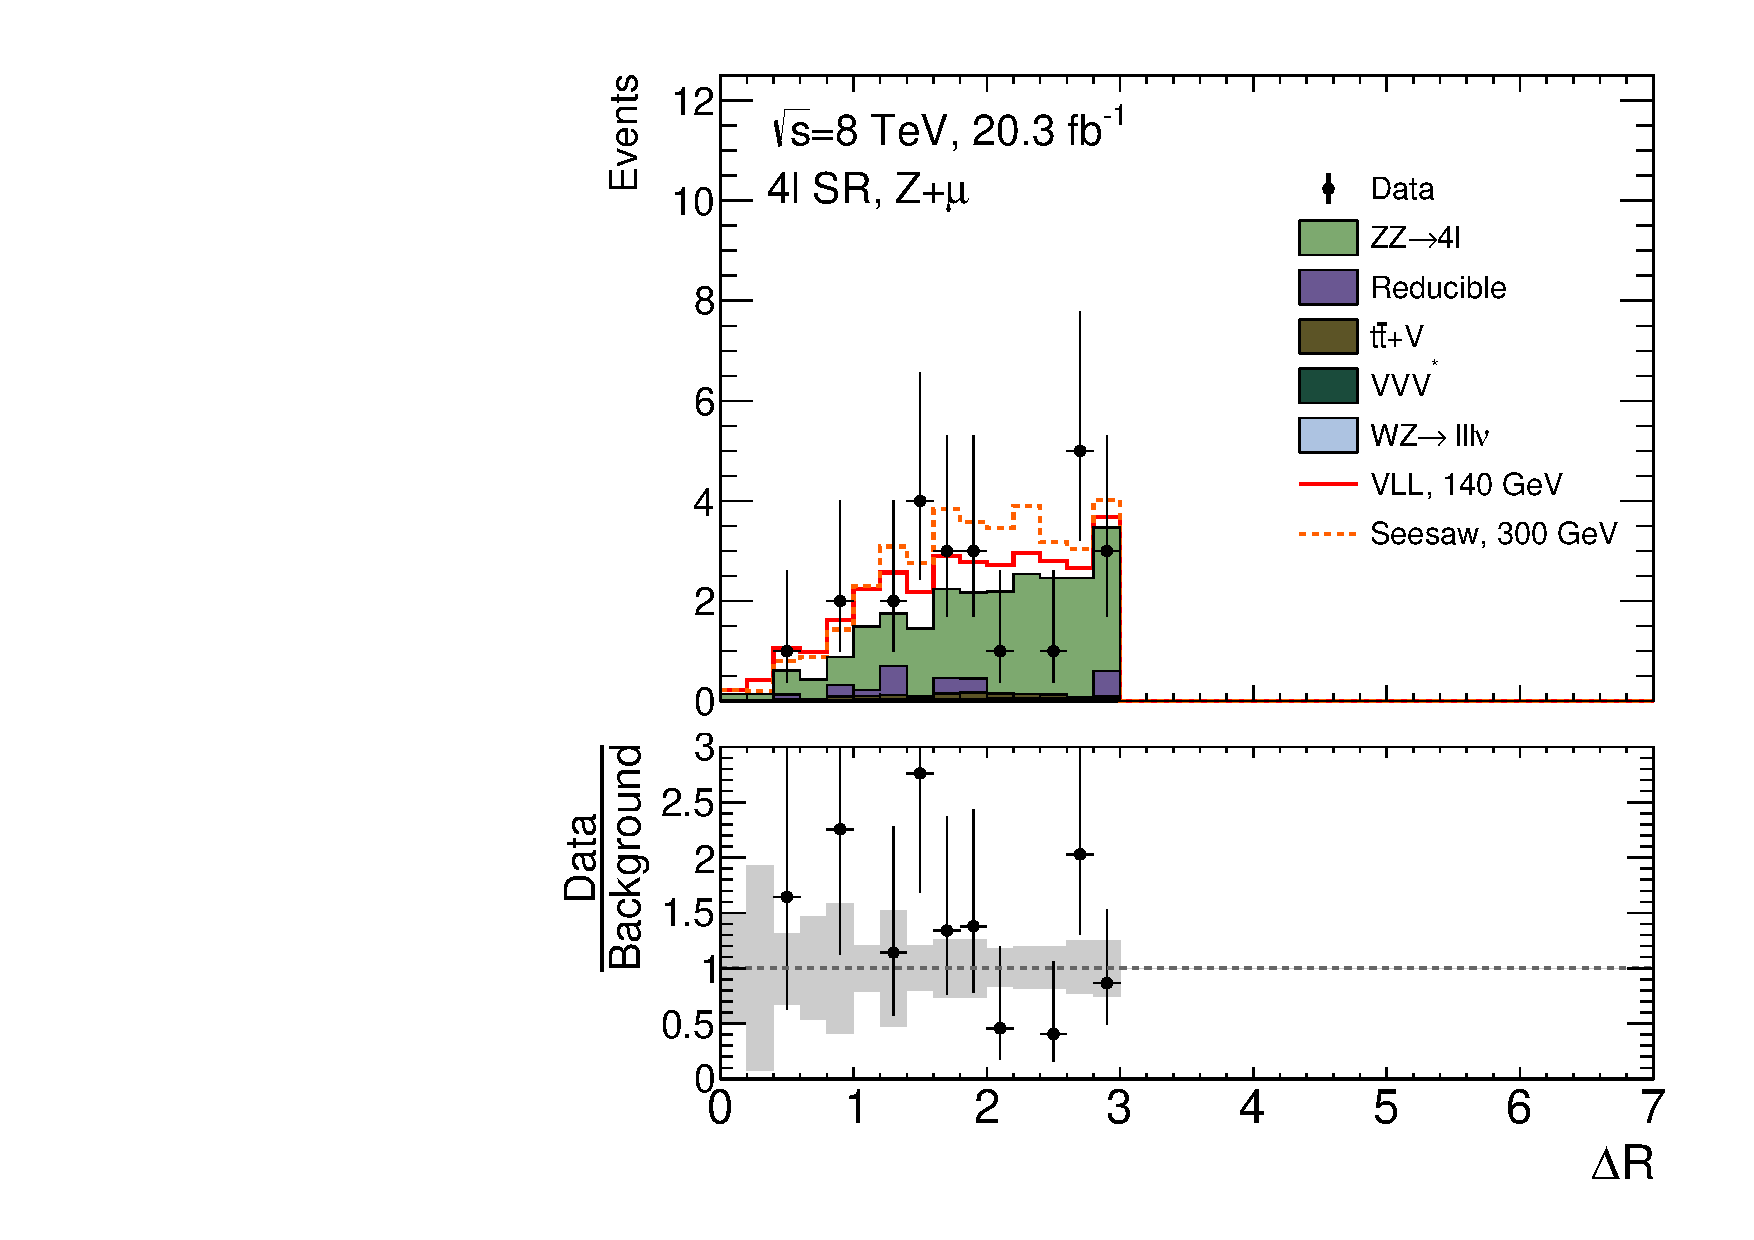
\includegraphics{figures/resonance/c_output_dR_Zmu_FourLNoM3L_300GeV}}
  } \\
  \caption{$\Delta R(Z,\ell_3)$ distributions for $Z+e$ and $Z+\mu$ candidates, for the inclusive and $\fourl$ signal regions (linear scale).}
  \label{fig:SR-dR-1-linear}
\end{figure}

\begin{figure}
  \centering
  \subfloat[ $Z+e$, dijet category] {
    \resizebox{0.48\textwidth}{!}{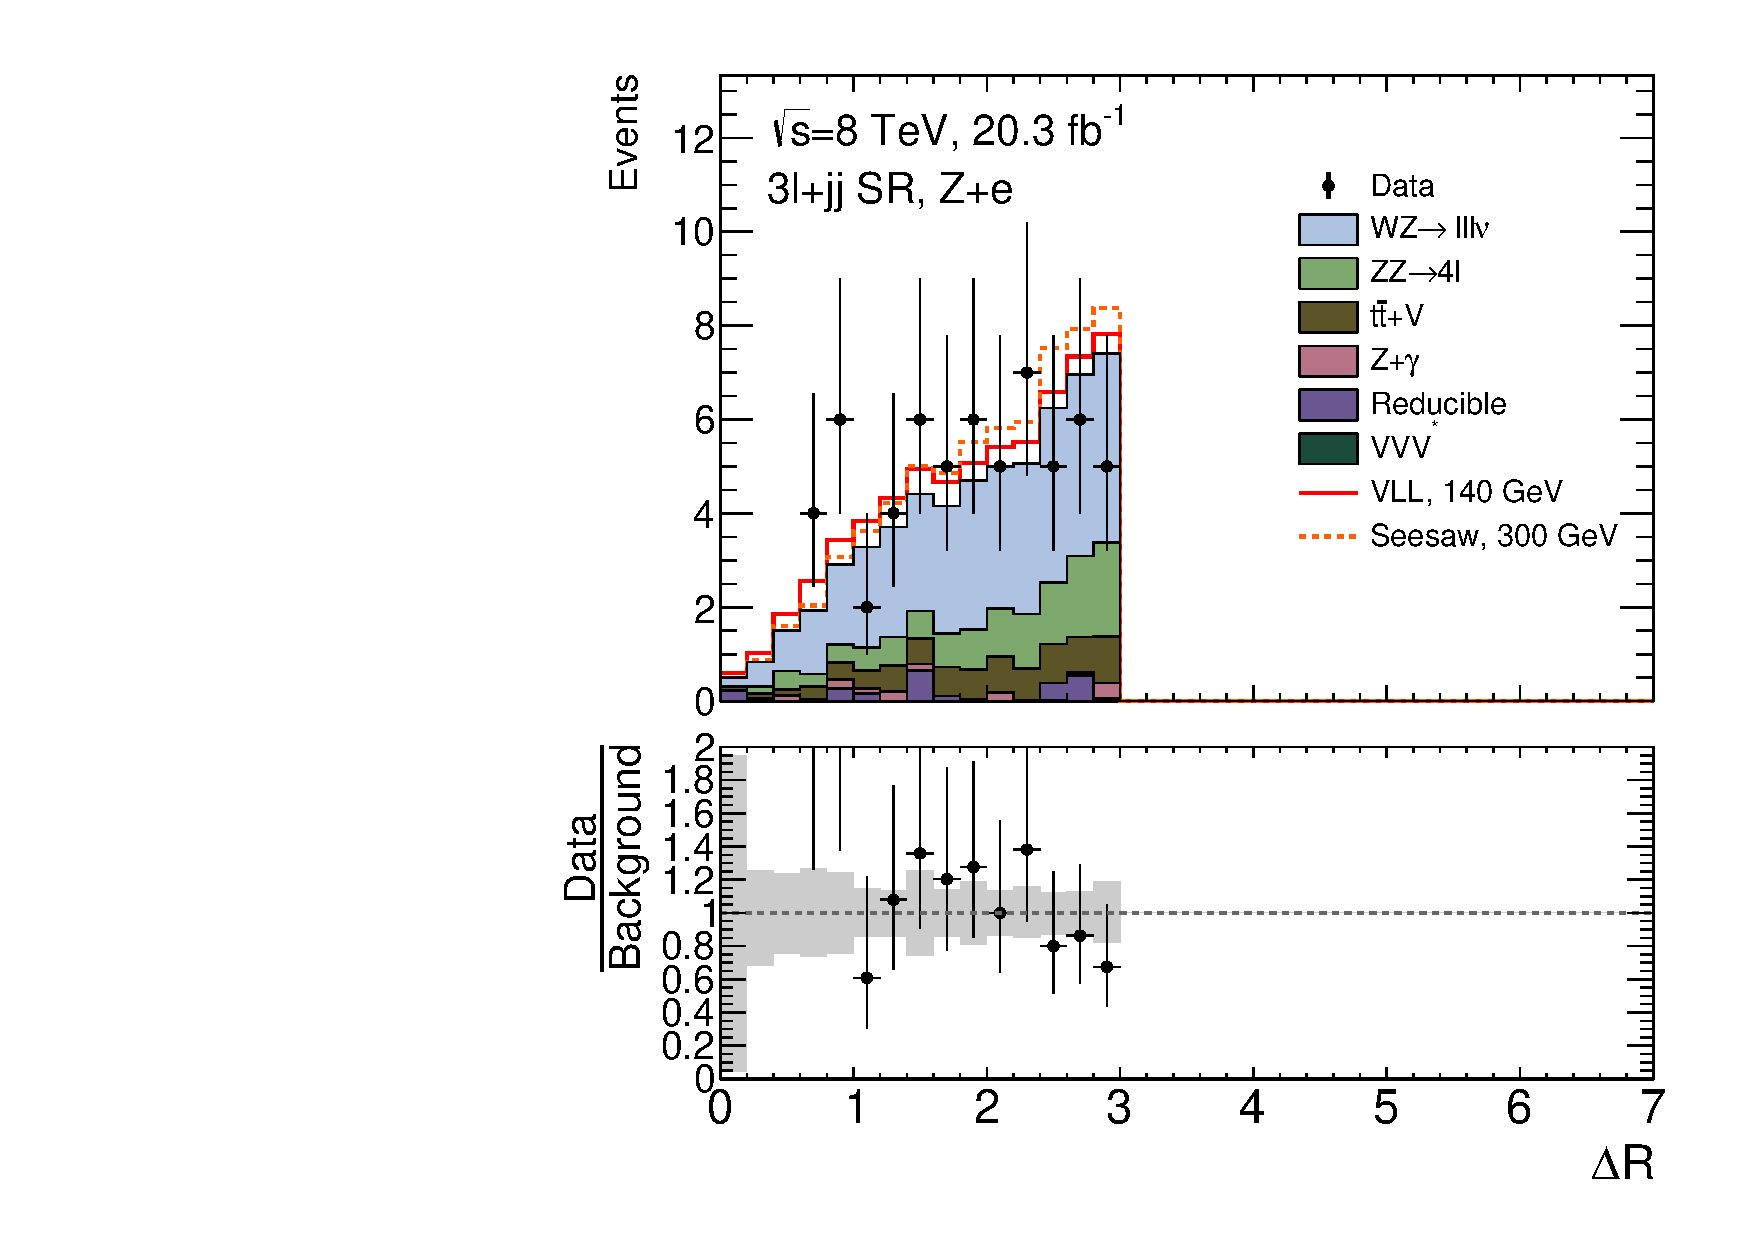
\includegraphics{figures/resonance/c_output_dR_Ze_ThreeLDijetNoM3L_300GeV}}
  }
  \subfloat[ $Z+\mu$, dijet category] {
    \resizebox{0.48\textwidth}{!}{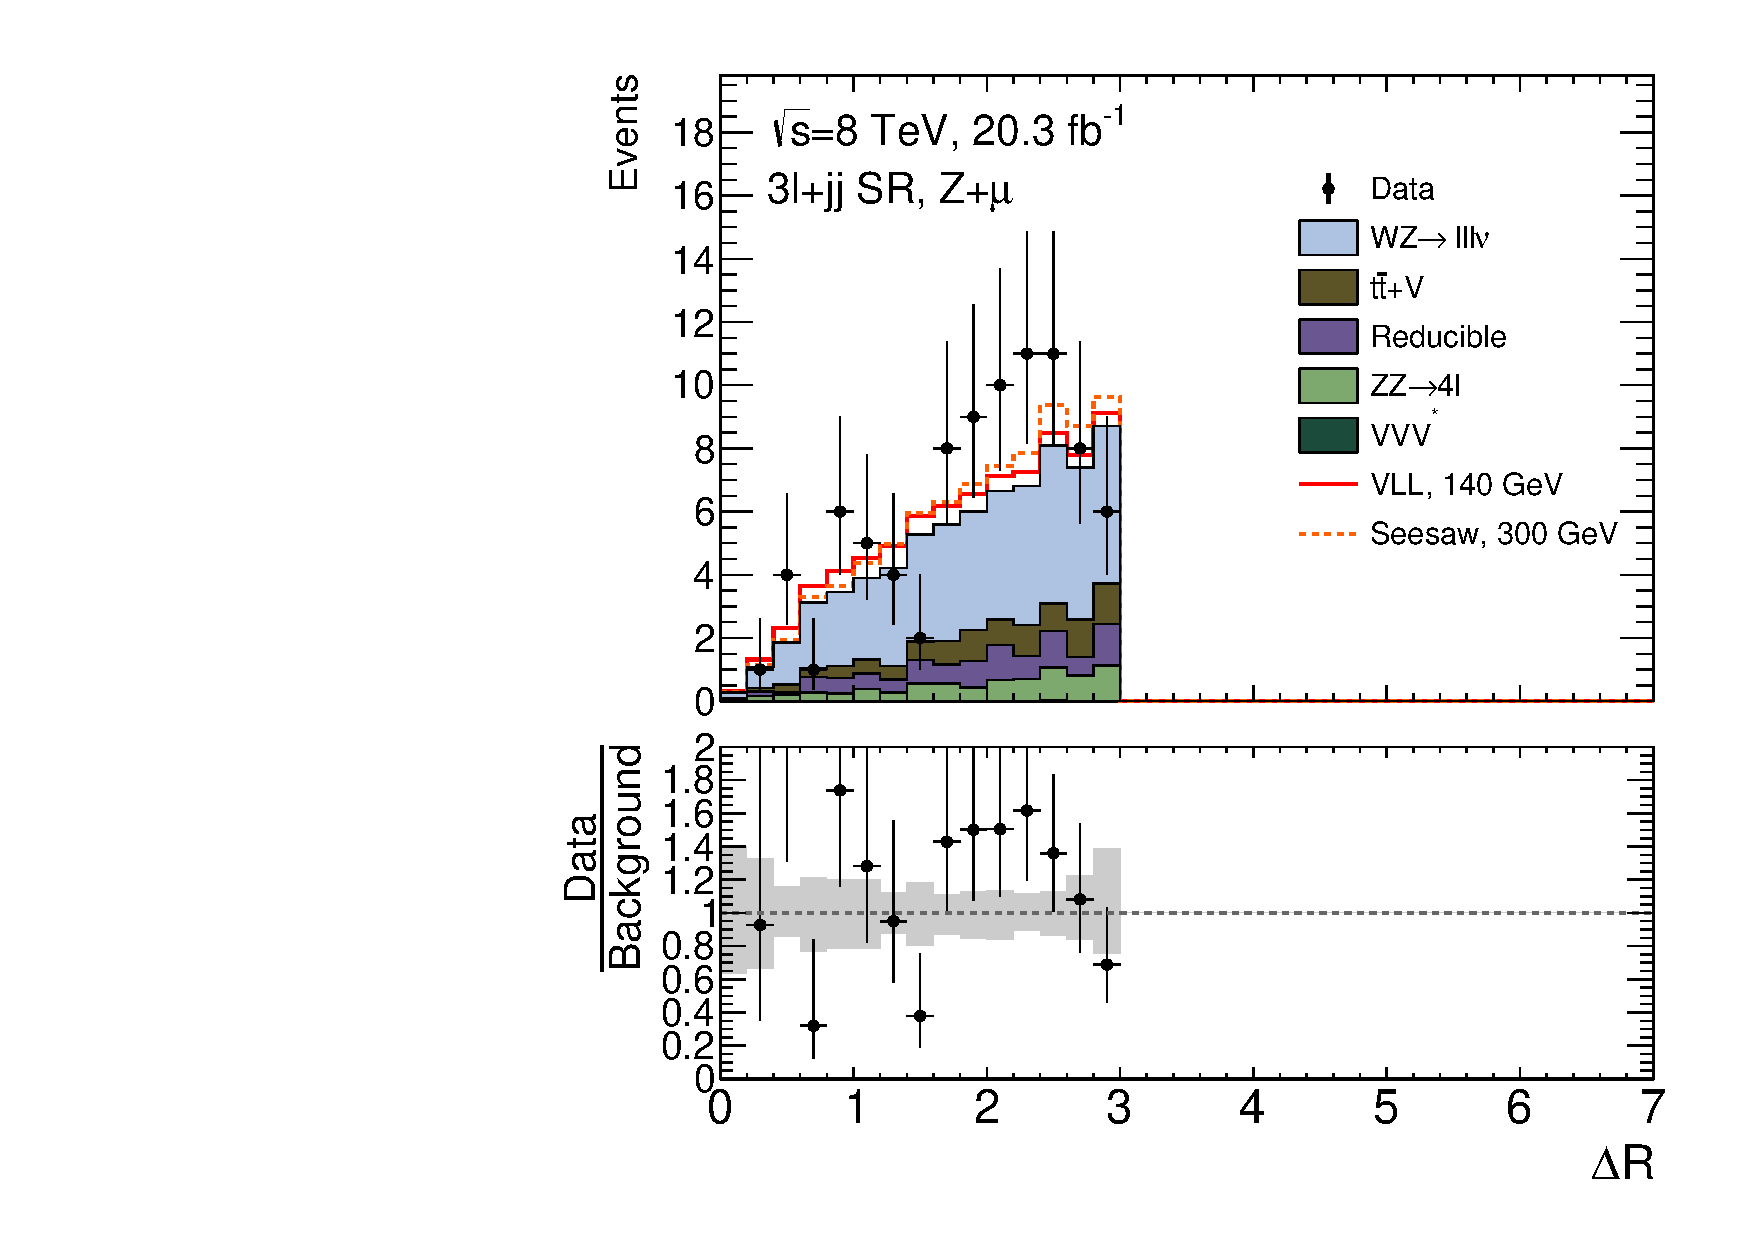
\includegraphics{figures/resonance/c_output_dR_Zmu_ThreeLDijetNoM3L_300GeV}}
  } \\
  \subfloat[ $Z+e$, else category] {
    \resizebox{0.48\textwidth}{!}{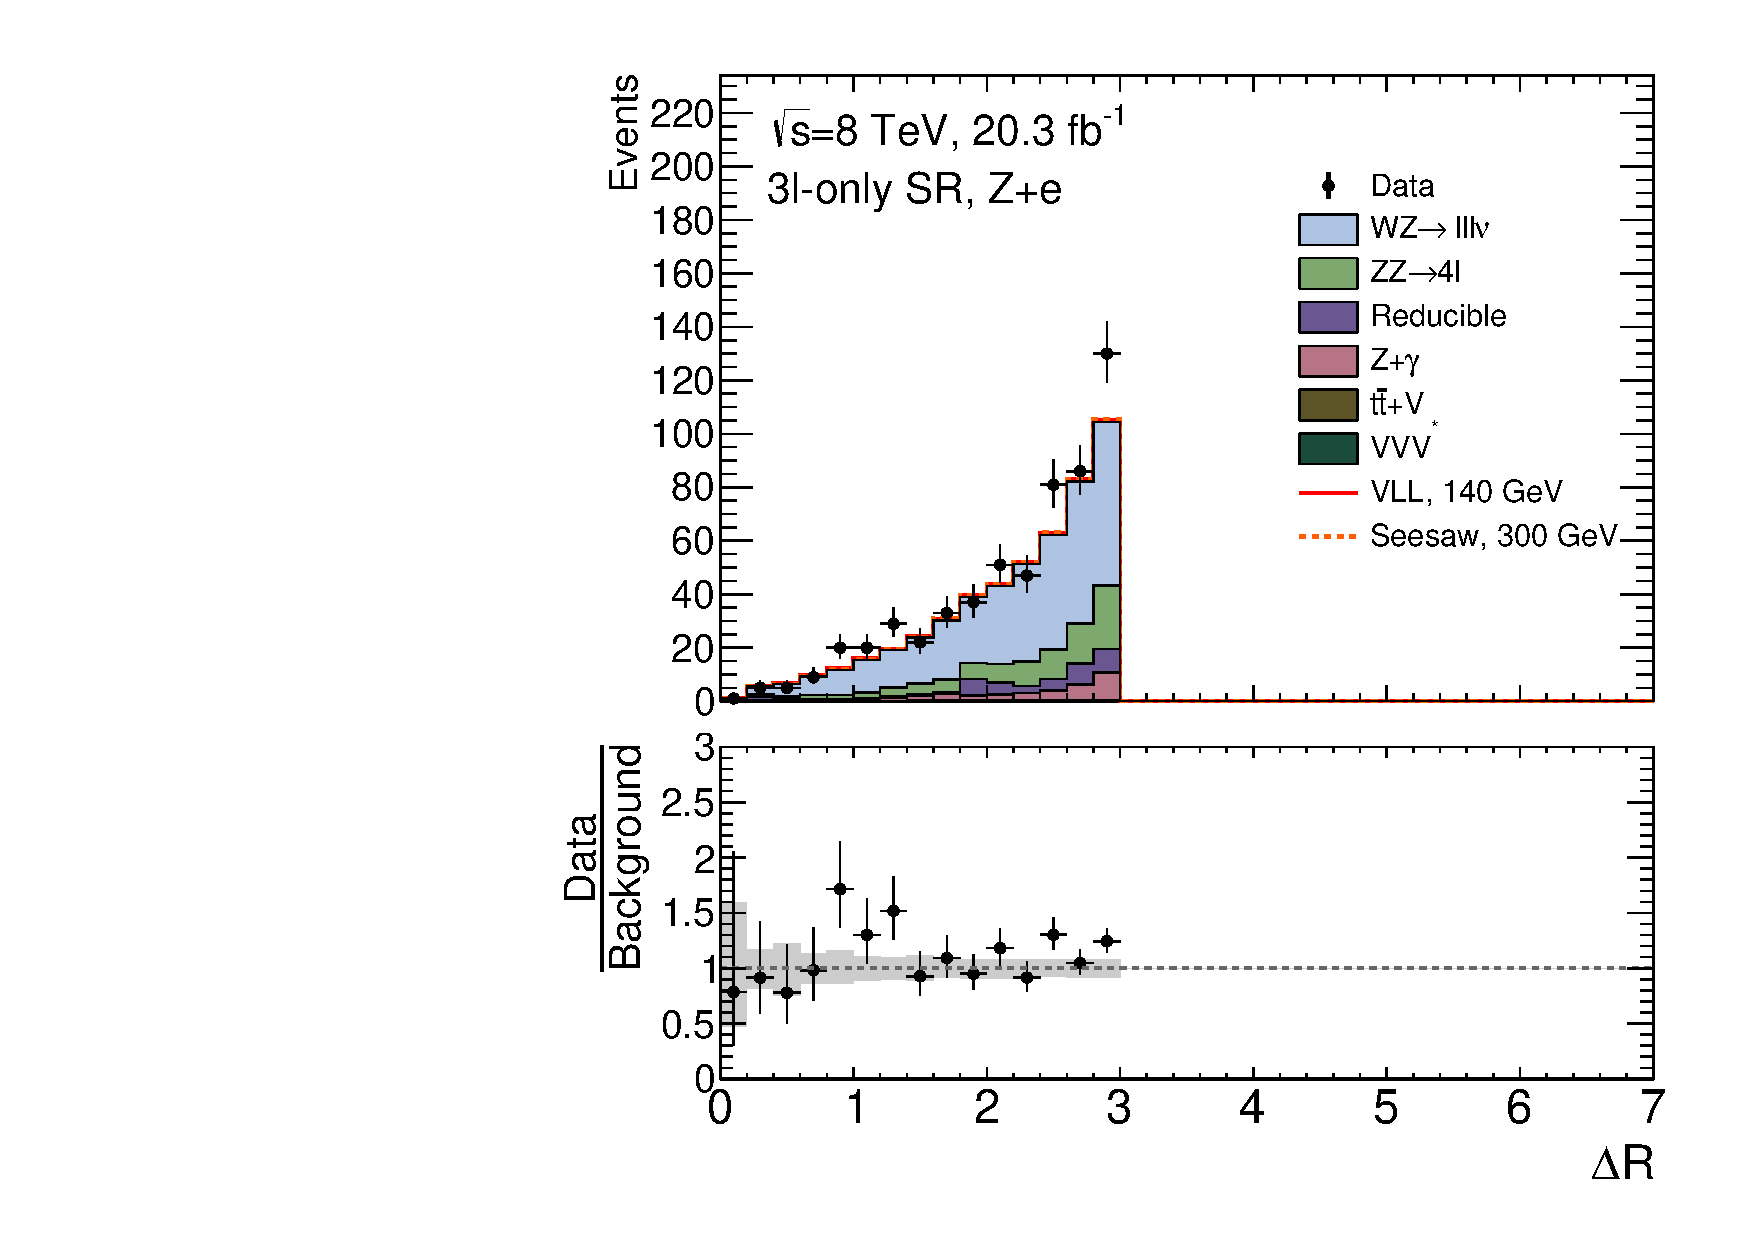
\includegraphics{figures/resonance/c_output_dR_Ze_ElseNoM3L_300GeV}}
  }
  \subfloat[ $Z+\mu$, else category] {
    \resizebox{0.48\textwidth}{!}{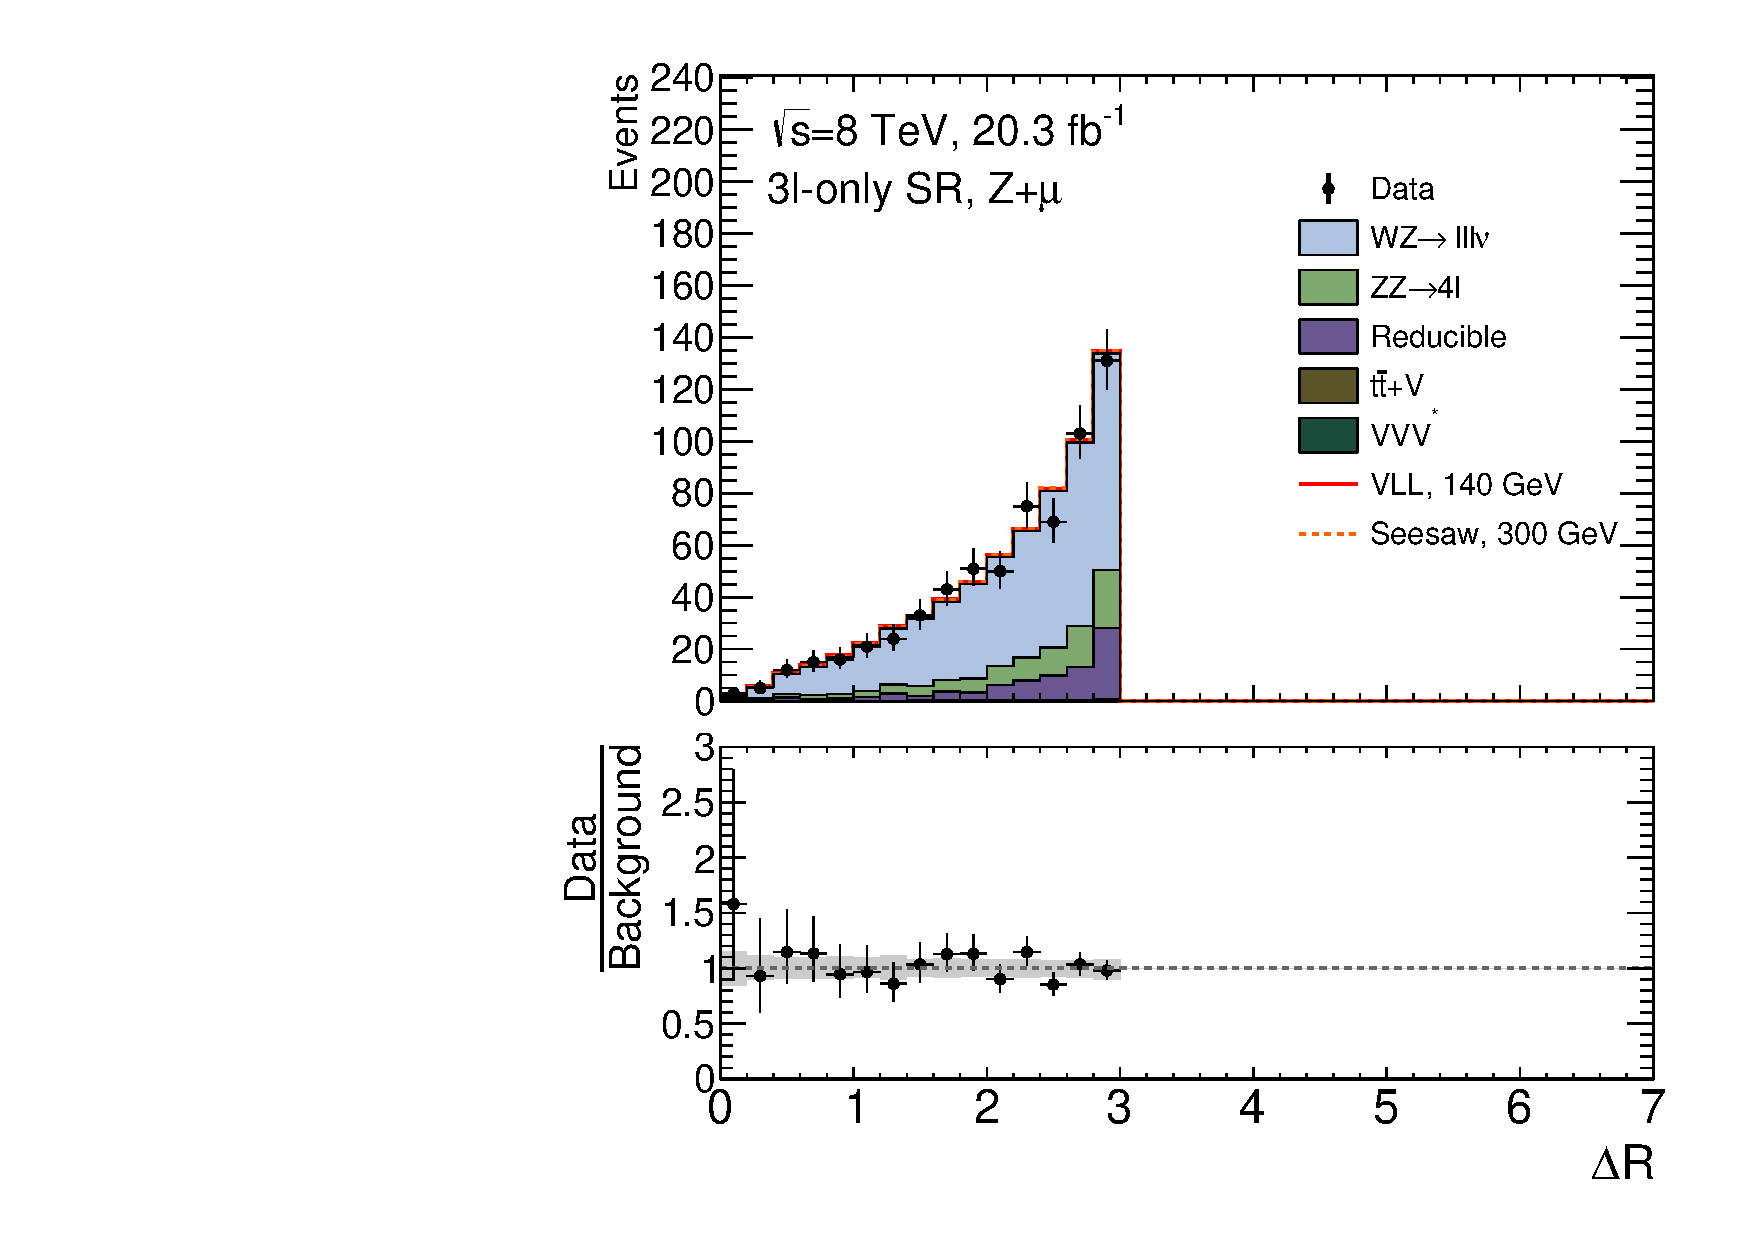
\includegraphics{figures/resonance/c_output_dR_Zmu_ElseNoM3L_300GeV}}
  }
  \caption{$\Delta R(Z,\ell_3)$ distributions for $Z+e$ and $Z+\mu$ candidates, for the $\threeljj$ and $\threelo$ signal regions (linear scale).}
  \label{fig:SR-dR-2-linear}
\end{figure}


\begin{figure}[htb]
  \centering
  \subfloat[ $Z+e$, inclusive] {
    \resizebox{0.48\textwidth}{!}{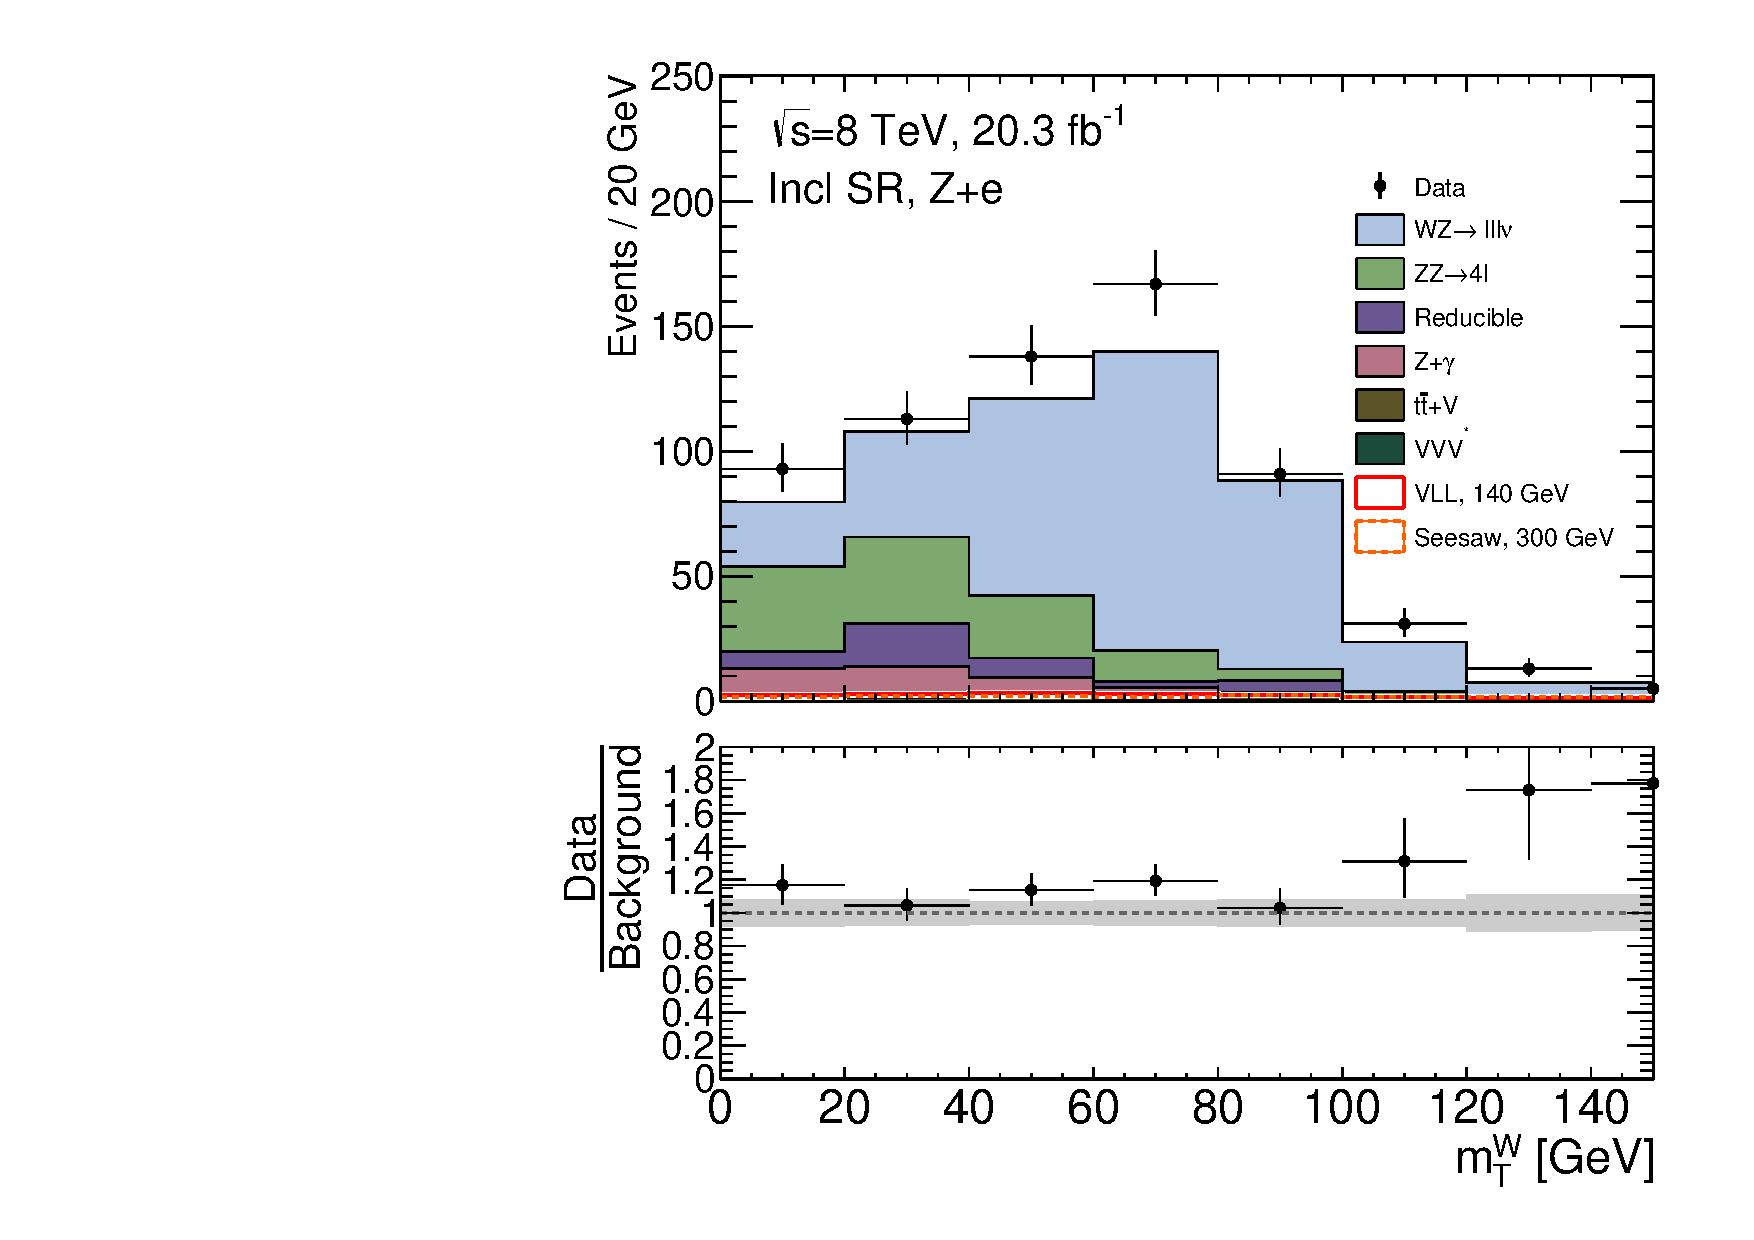
\includegraphics{figures/resonance/c_output_mTW_Ze_InclusiveNoM3L_300GeV}}
  }
  \subfloat[ $Z+\mu$, inclusive] {
    \resizebox{0.48\textwidth}{!}{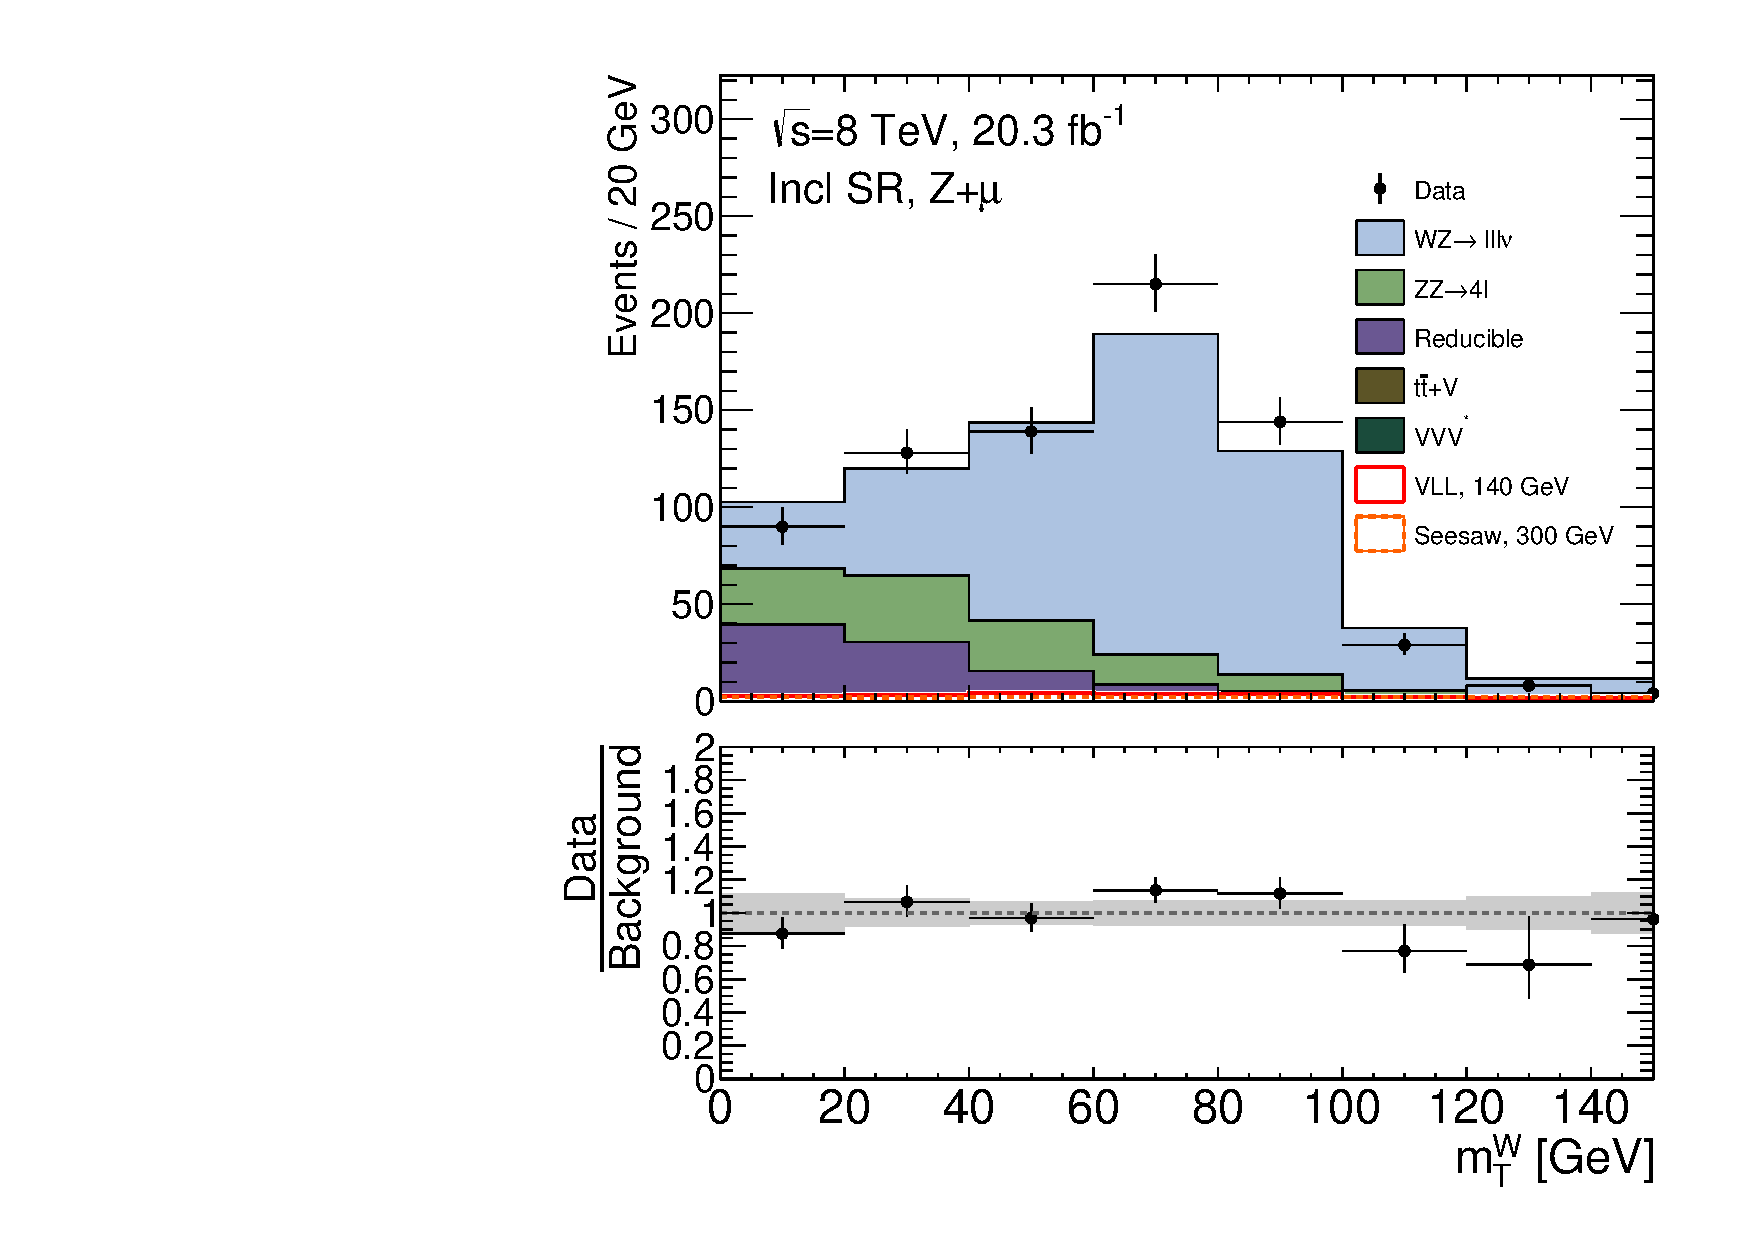
\includegraphics{figures/resonance/c_output_mTW_Zmu_InclusiveNoM3L_300GeV}}
  } \\
  \subfloat[ $Z+e$, $4L$ category] {
    \resizebox{0.48\textwidth}{!}{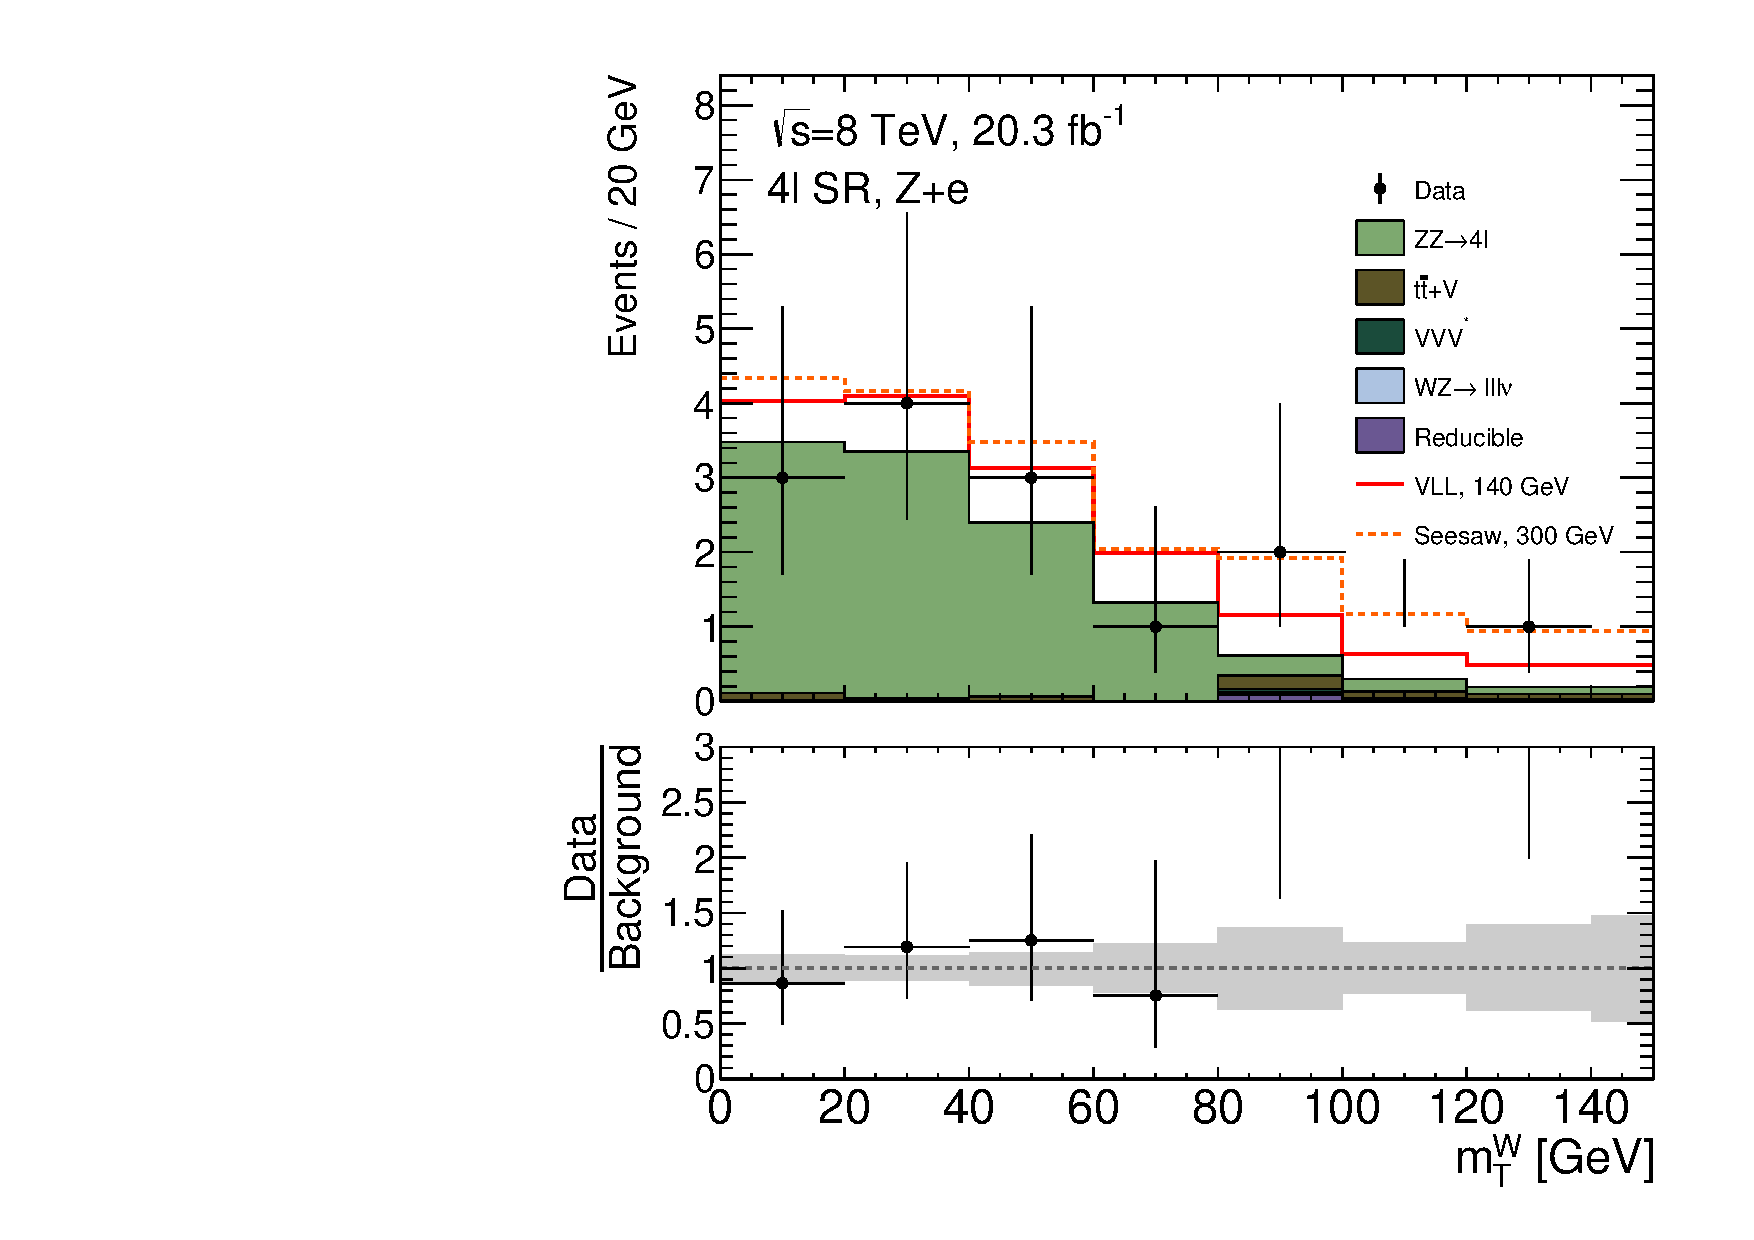
\includegraphics{figures/resonance/c_output_mTW_Ze_FourLNoM3L_300GeV}}
  }
  \subfloat[ $Z+\mu$, $4L$ category] {
    \resizebox{0.48\textwidth}{!}{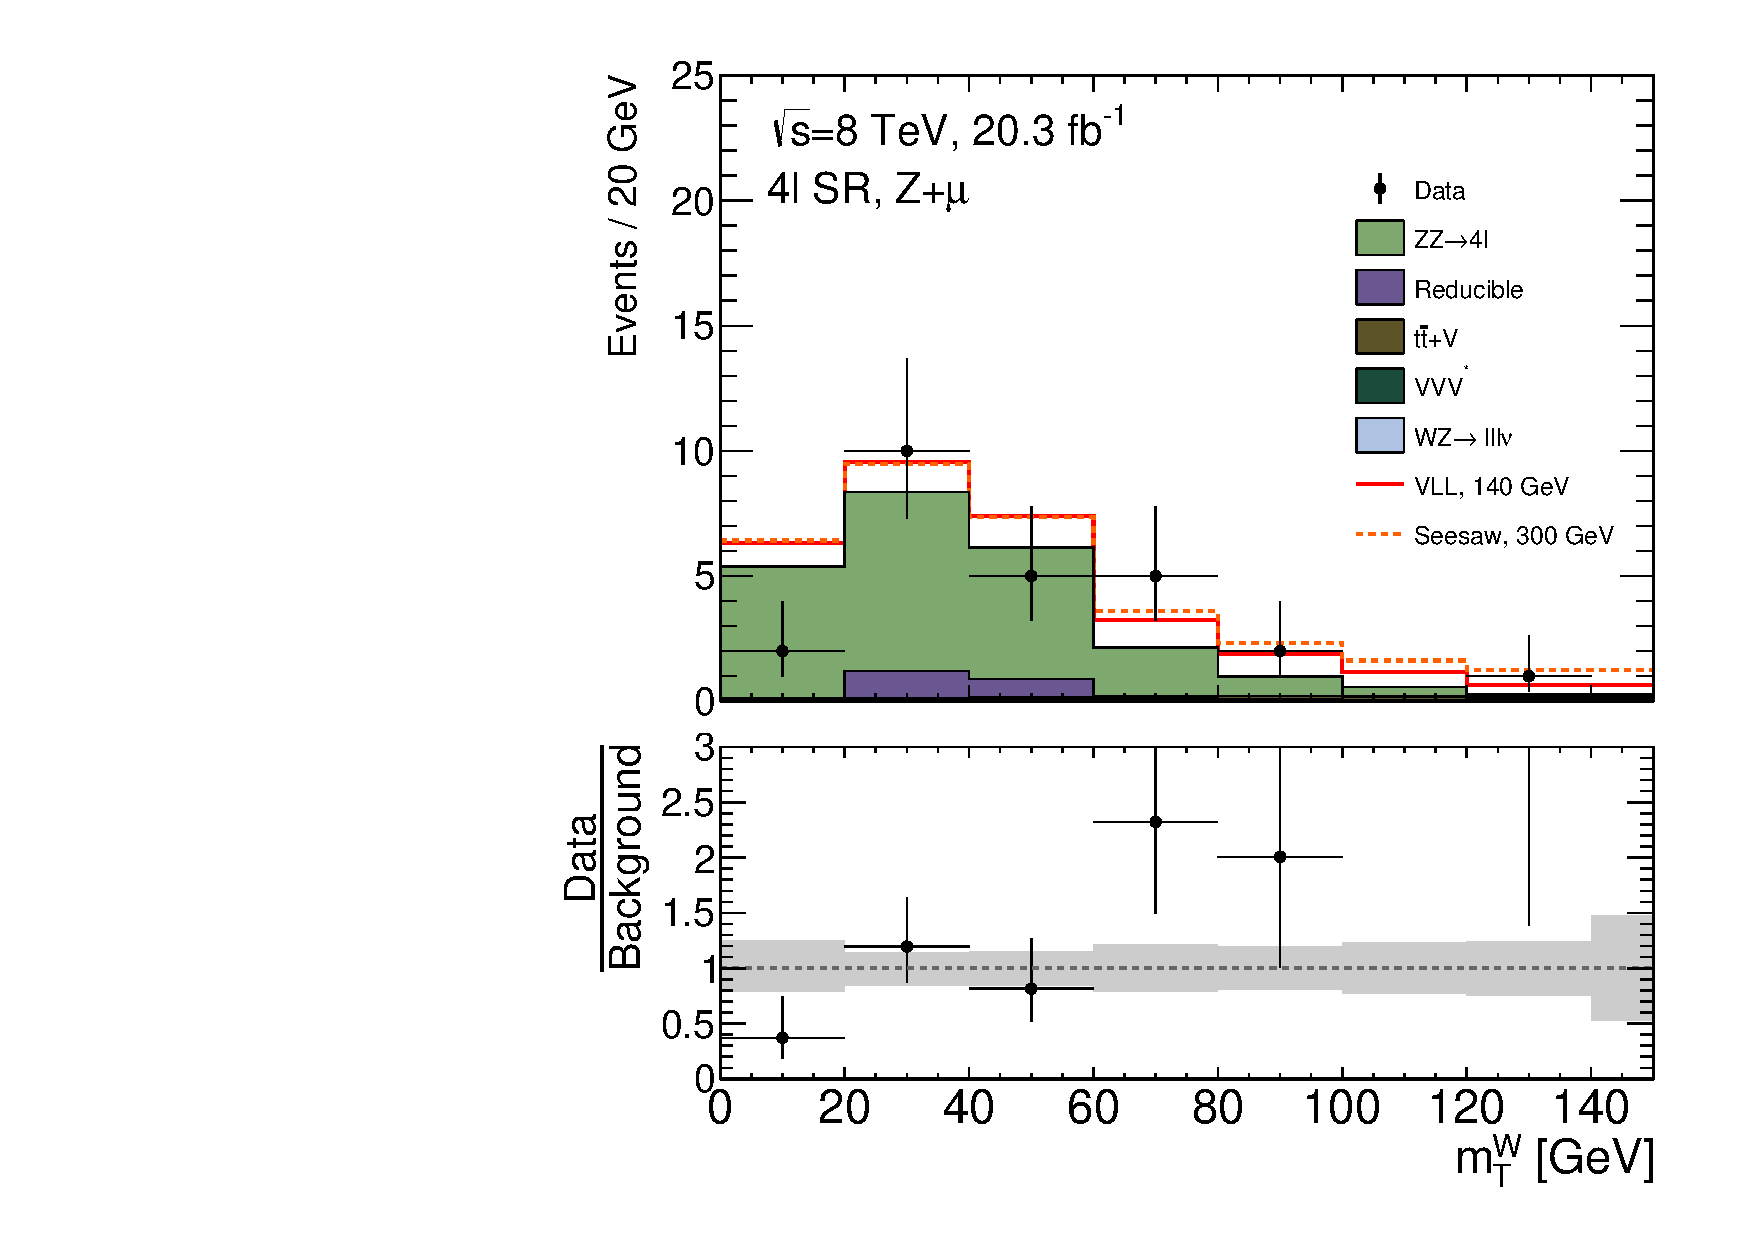
\includegraphics{figures/resonance/c_output_mTW_Zmu_FourLNoM3L_300GeV}}
  } \\
  \caption{Transverse mass of the missing energy and bachelor lepton ($\mtw$) for $Z+e$ and $Z+\mu$ candidates, for the inclusive and $\fourl$ signal regions.}
  \label{fig:SR-mTW-1}
\end{figure}

\clearpage

\begin{figure}[htb]
  \centering
  \subfloat[ $Z+e$, dijet category] {
    \resizebox{0.48\textwidth}{!}{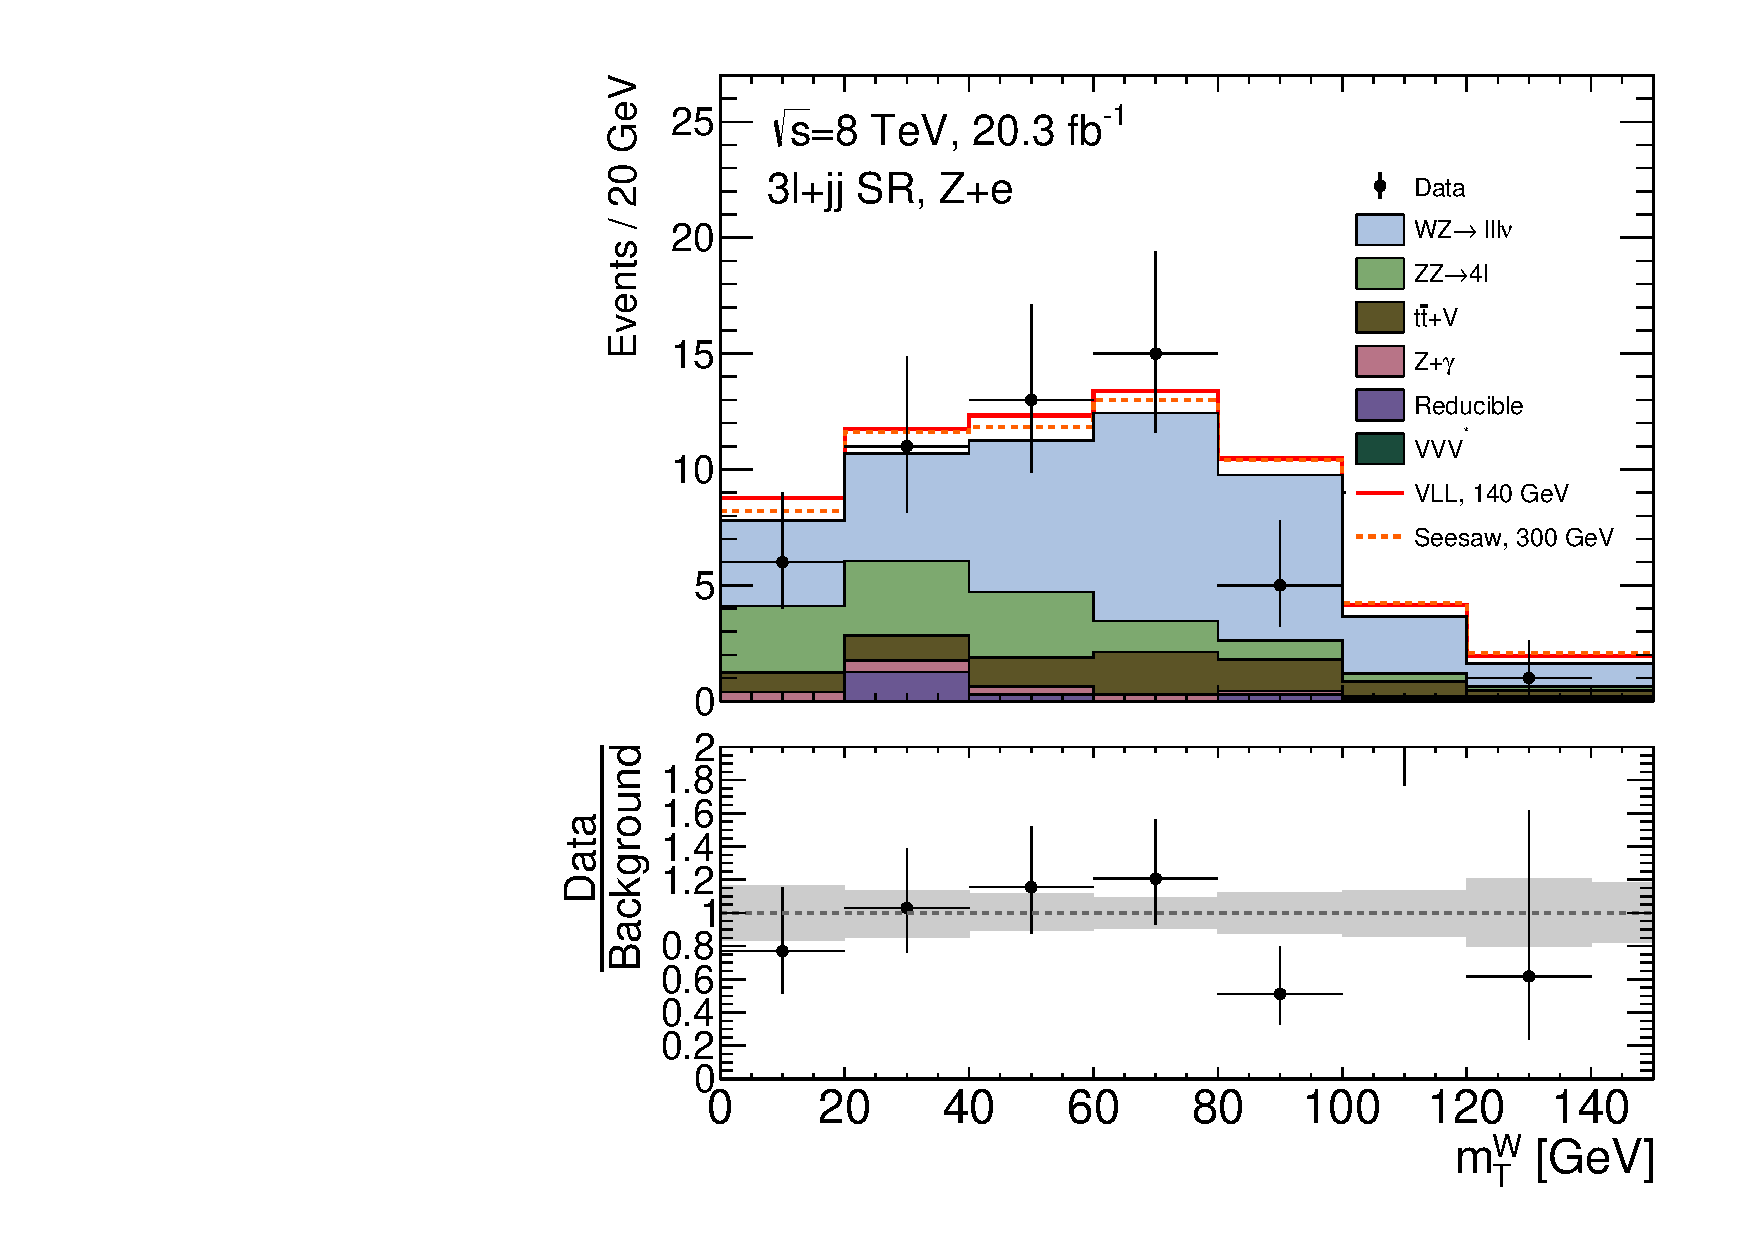
\includegraphics{figures/resonance/c_output_mTW_Ze_ThreeLDijetNoM3L_300GeV}}
  }
  \subfloat[ $Z+\mu$, dijet category] {
    \resizebox{0.48\textwidth}{!}{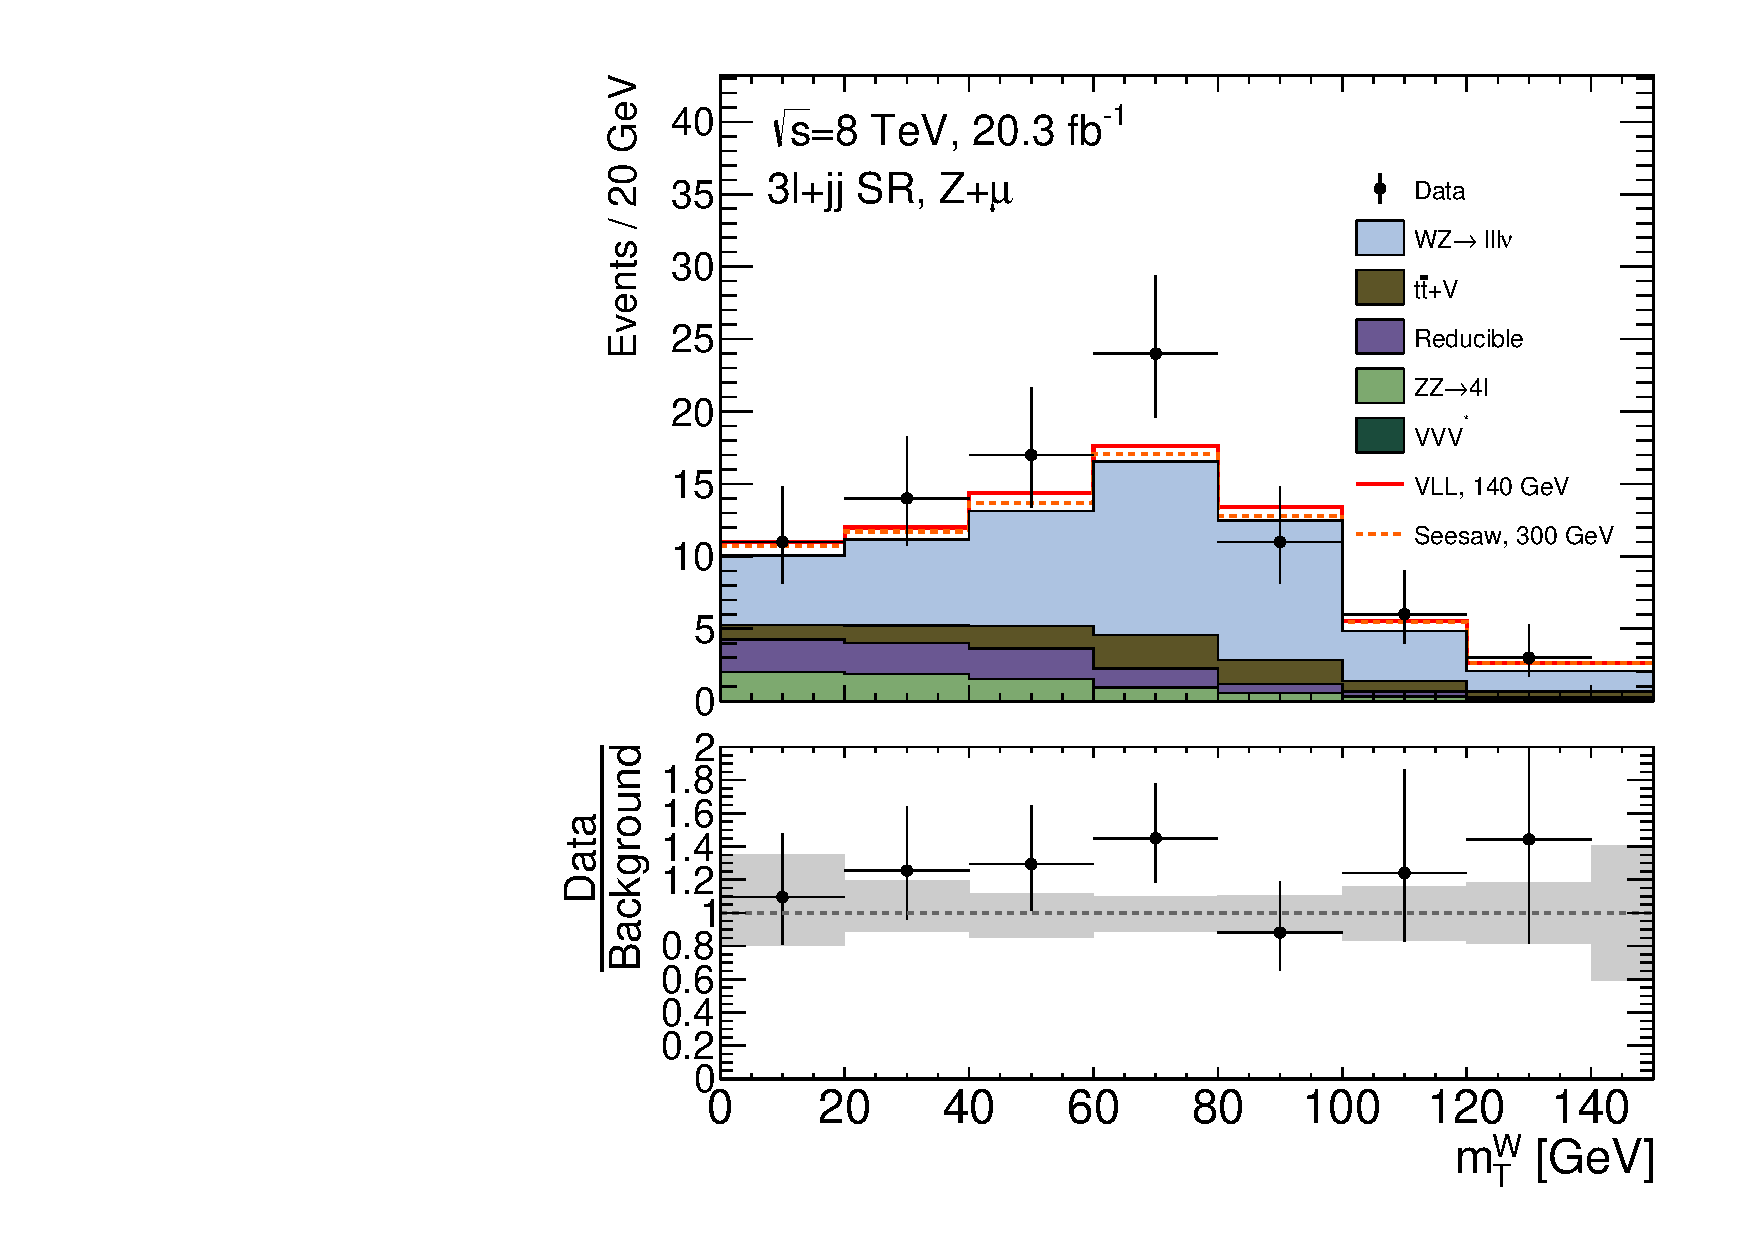
\includegraphics{figures/resonance/c_output_mTW_Zmu_ThreeLDijetNoM3L_300GeV}}
  } \\
  \subfloat[ $Z+e$, else category] {
    \resizebox{0.48\textwidth}{!}{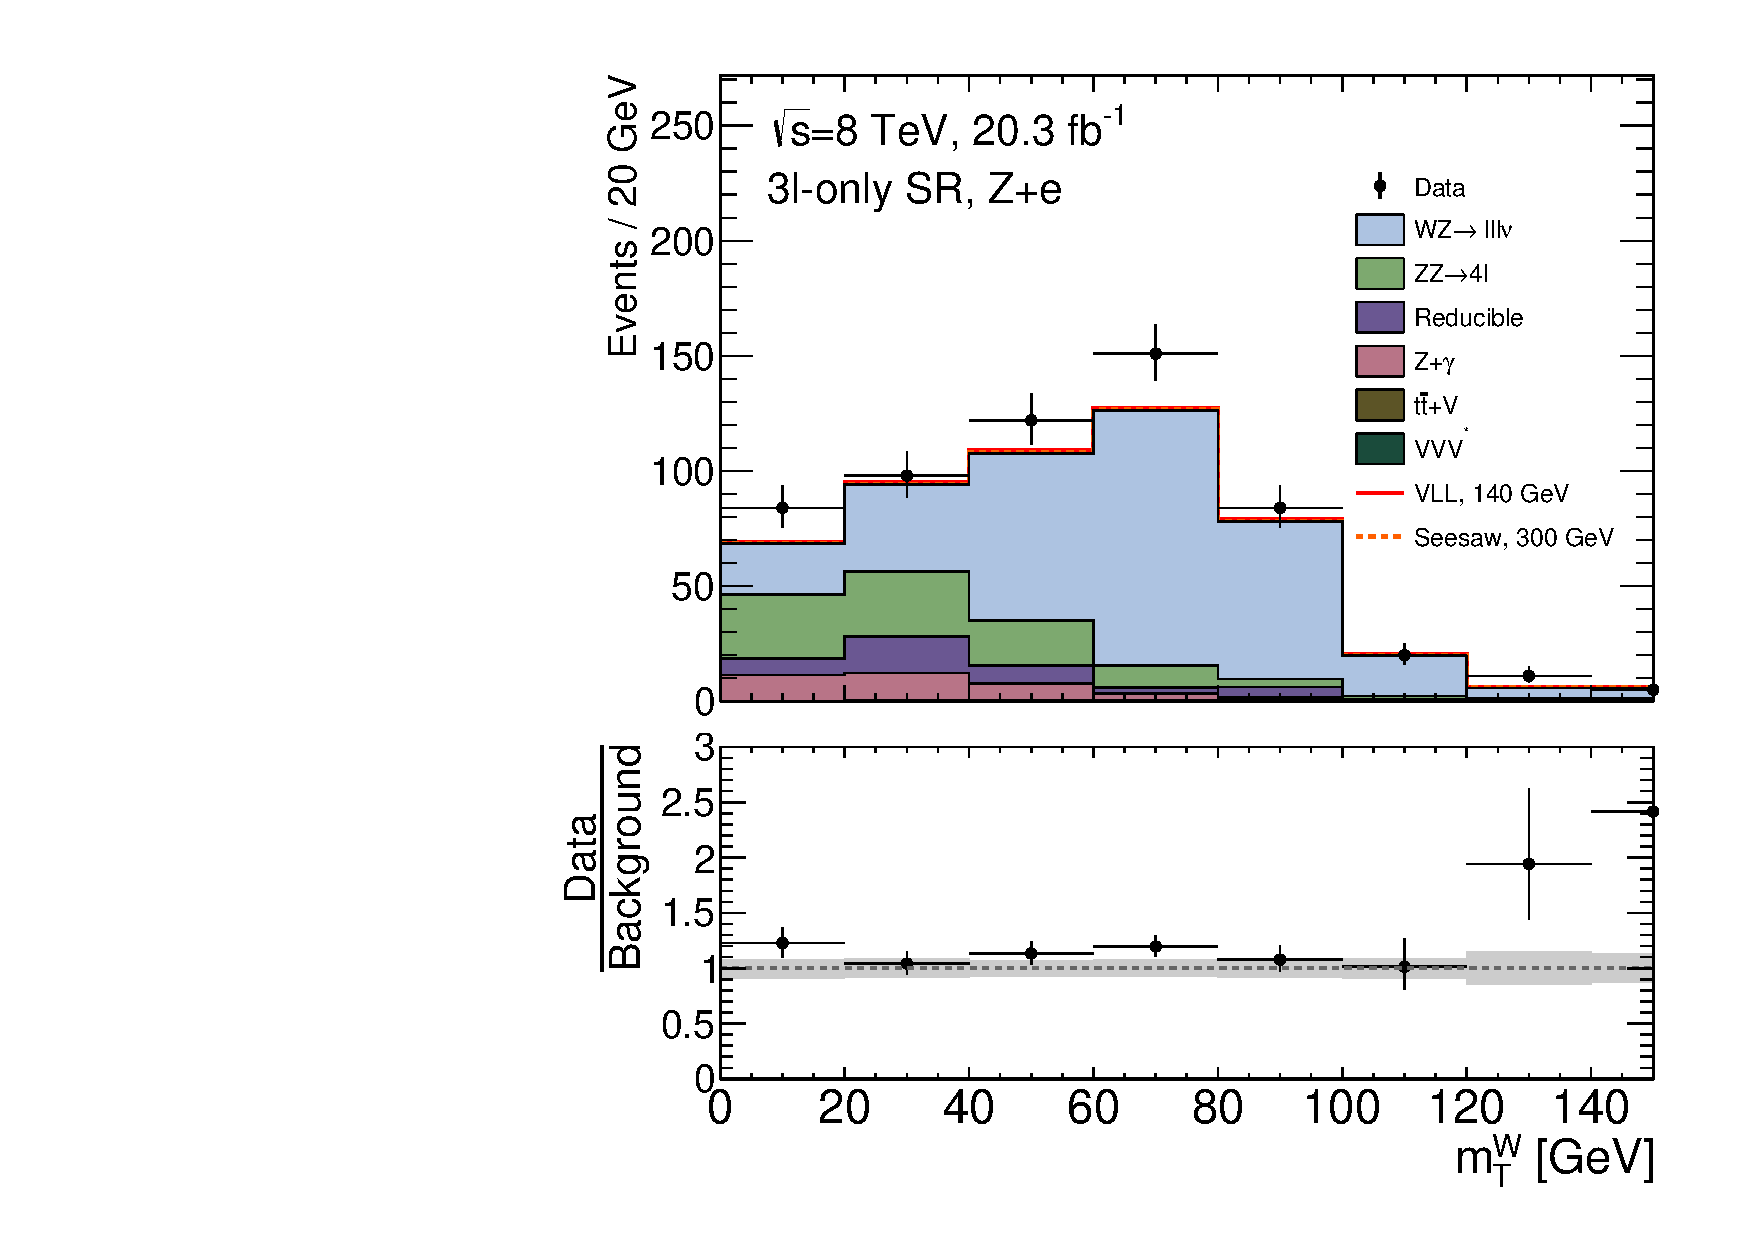
\includegraphics{figures/resonance/c_output_mTW_Ze_ElseNoM3L_300GeV}}
  }
  \subfloat[ $Z+\mu$, else category] {
    \resizebox{0.48\textwidth}{!}{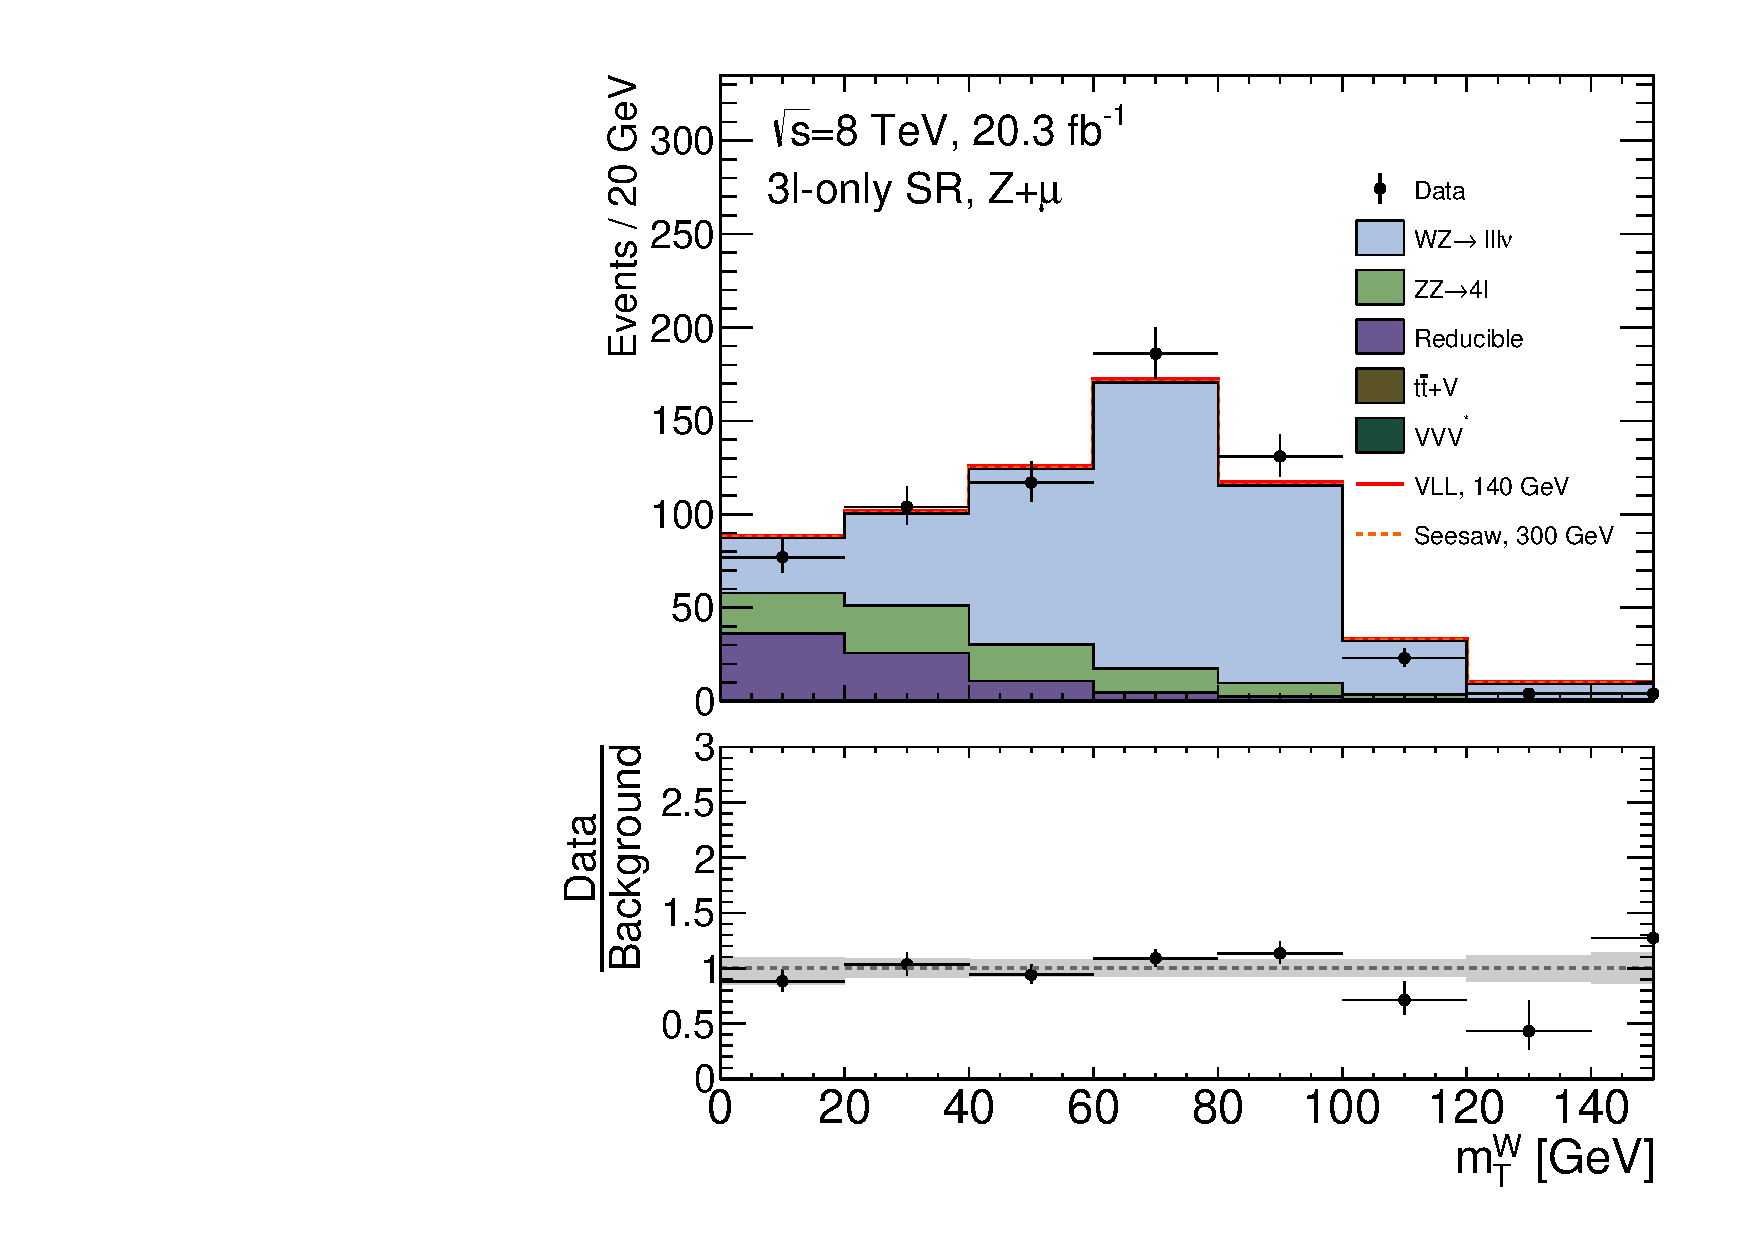
\includegraphics{figures/resonance/c_output_mTW_Zmu_ElseNoM3L_300GeV}}
  }
  \caption{Transverse mass of the missing energy and bachelor lepton ($\mtw$) for $Z+e$ and $Z+\mu$ candidates, for the $\threeljj$ and $\threelo$ signal regions.}
  \label{fig:SR-mTW-2}
\end{figure}

\clearpage

\begin{figure}[htb]
  \centering
  \subfloat[ $Z+e$, inclusive] {
    \resizebox{0.48\textwidth}{!}{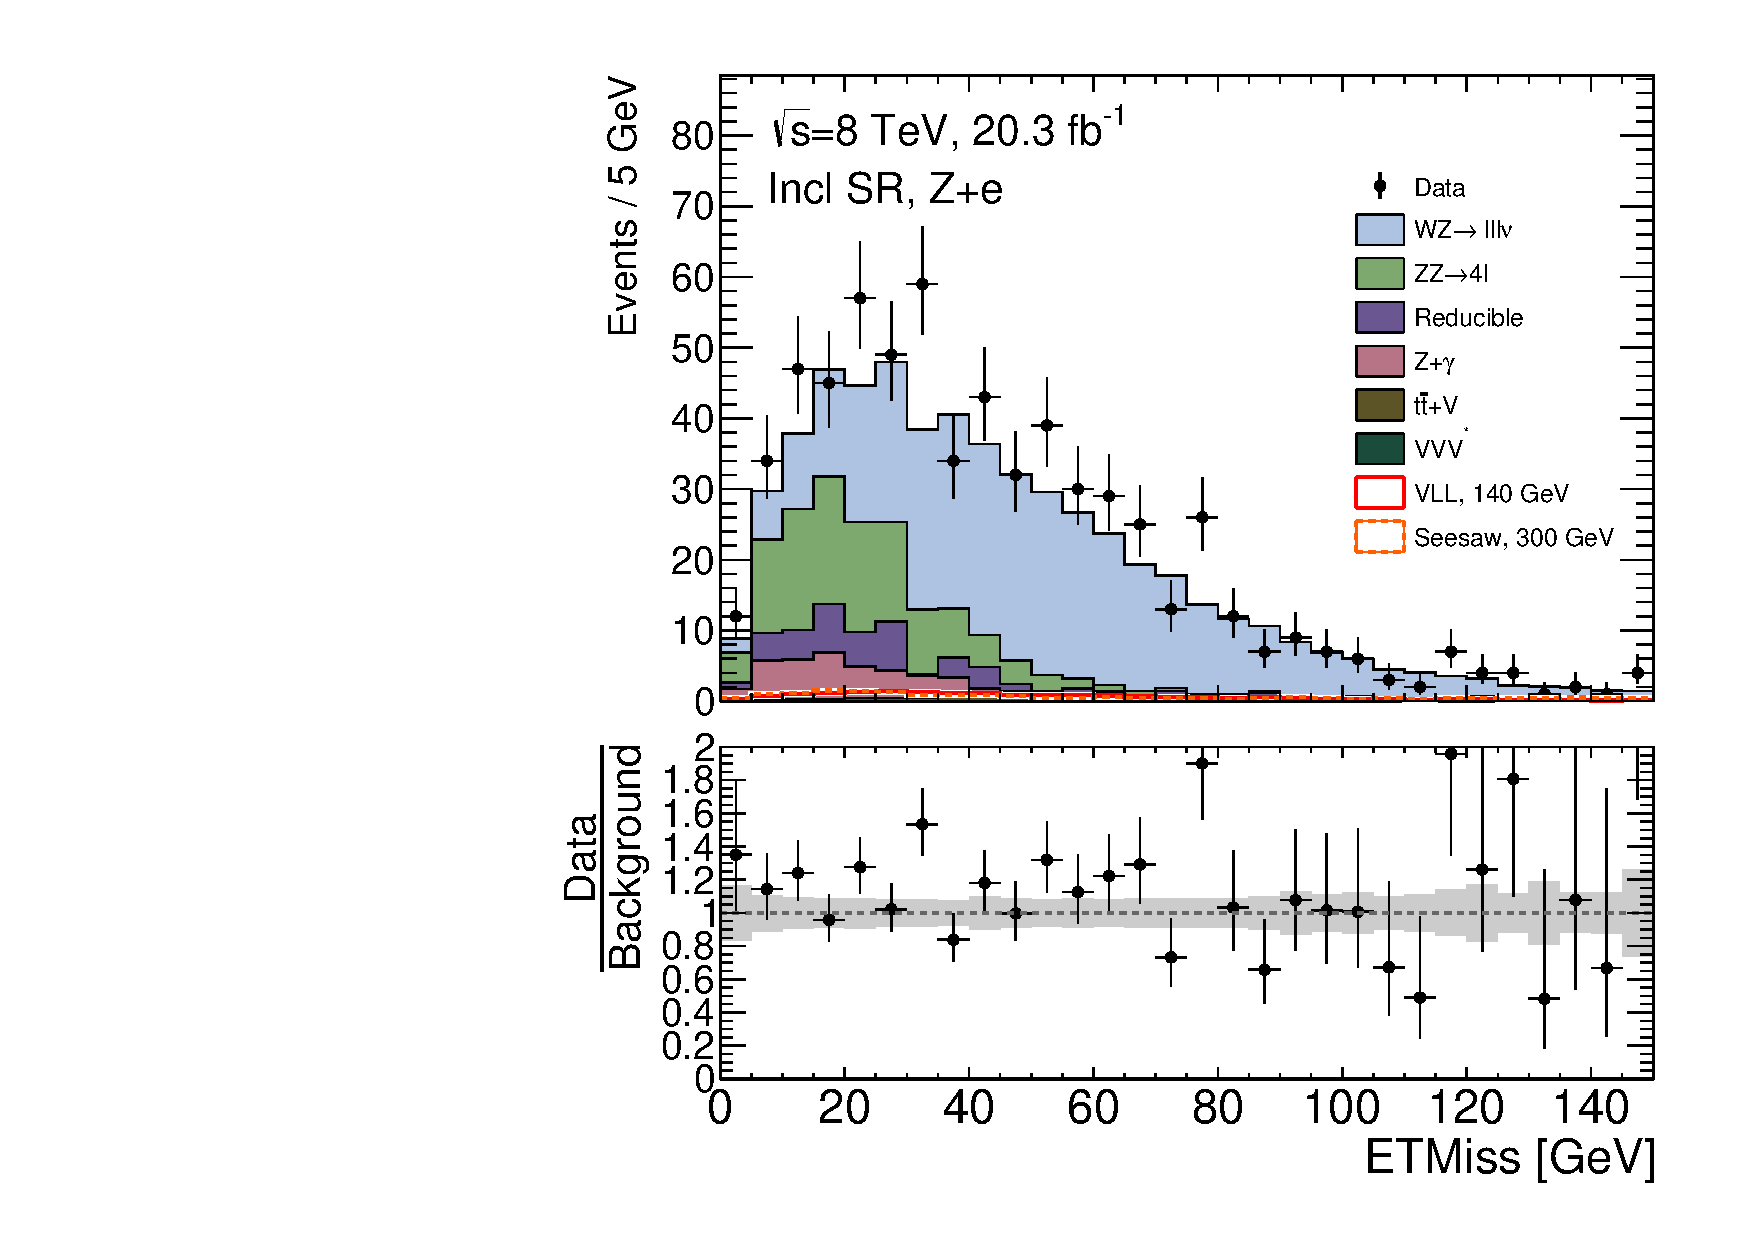
\includegraphics{figures/resonance/c_output_ETMiss_Ze_InclusiveNoM3L_300GeV}}
  }
  \subfloat[ $Z+\mu$, inclusive] {
    \resizebox{0.48\textwidth}{!}{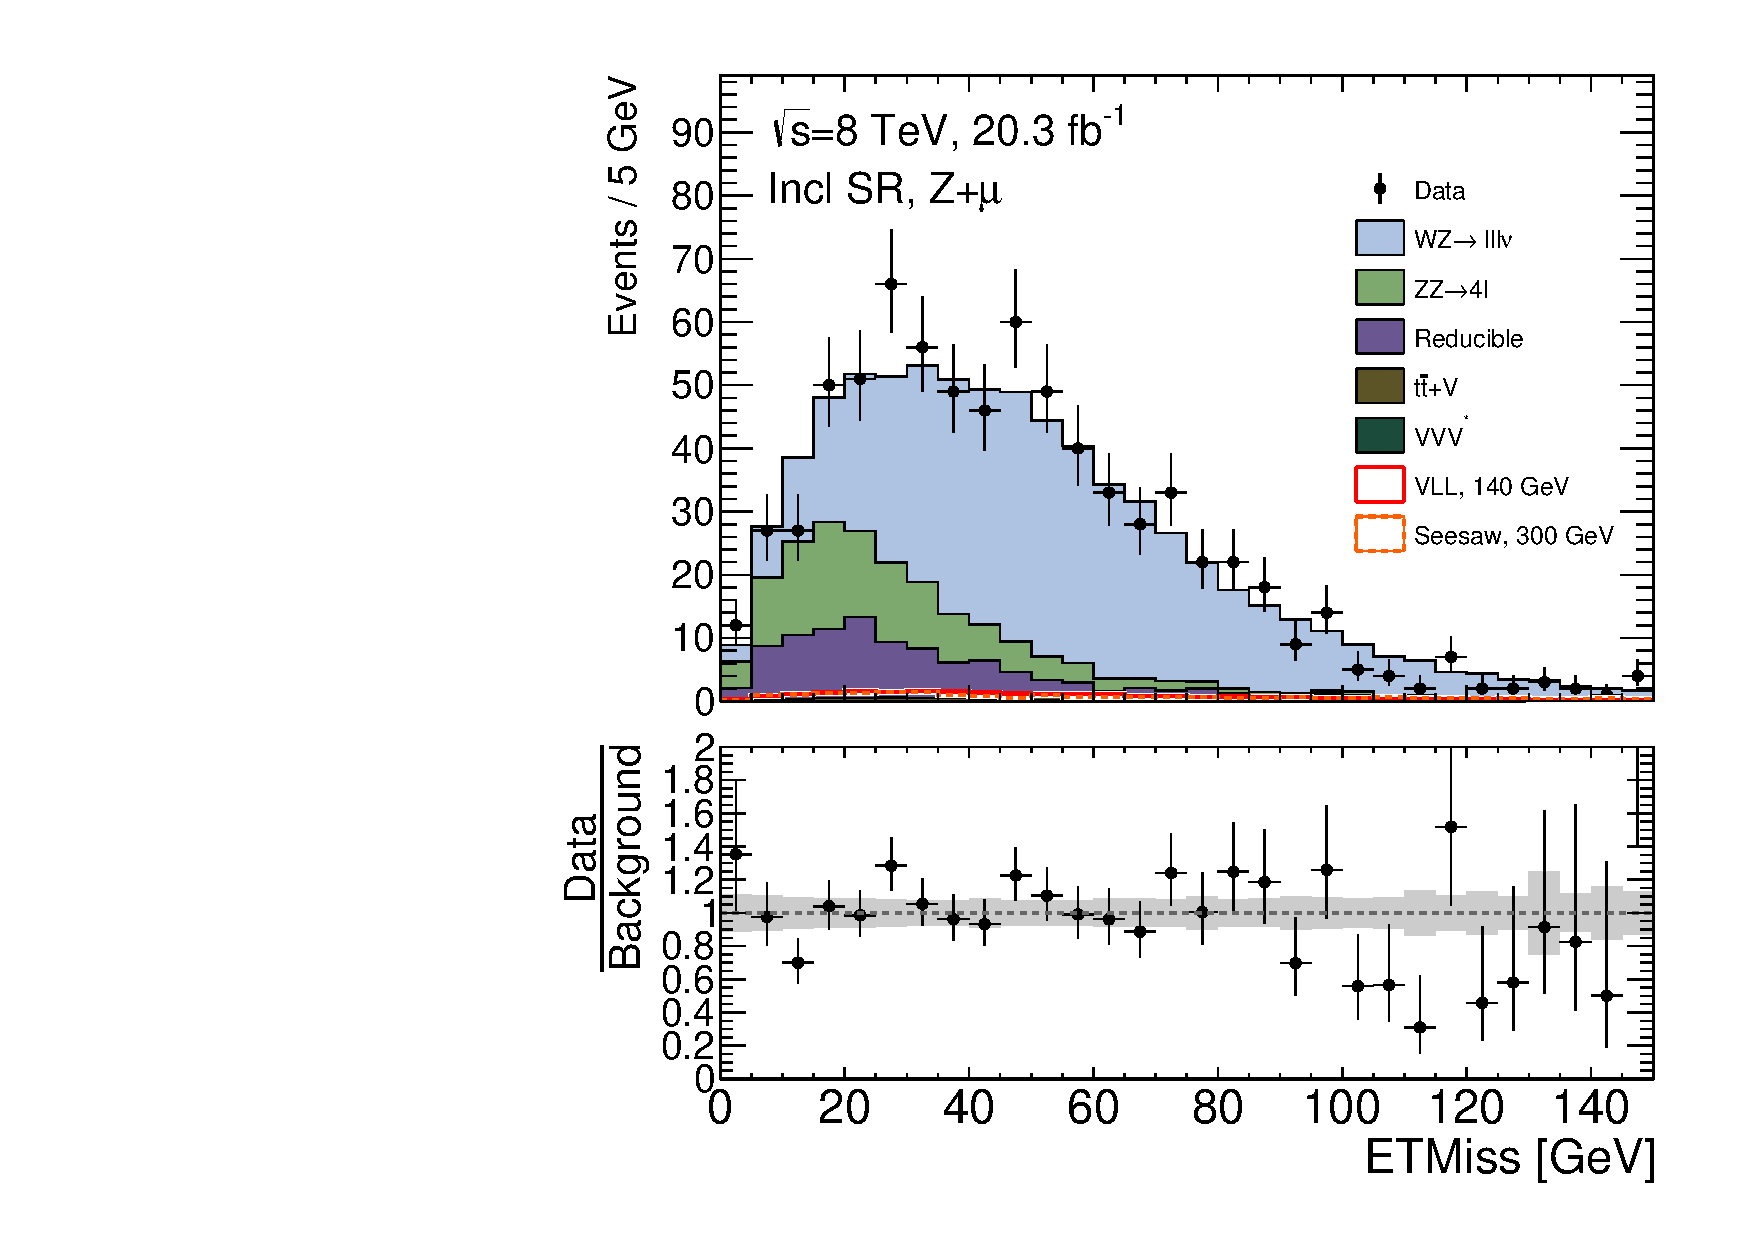
\includegraphics{figures/resonance/c_output_ETMiss_Zmu_InclusiveNoM3L_300GeV}}
  } \\
  \subfloat[ $Z+e$, $4L$ category] {
    \resizebox{0.48\textwidth}{!}{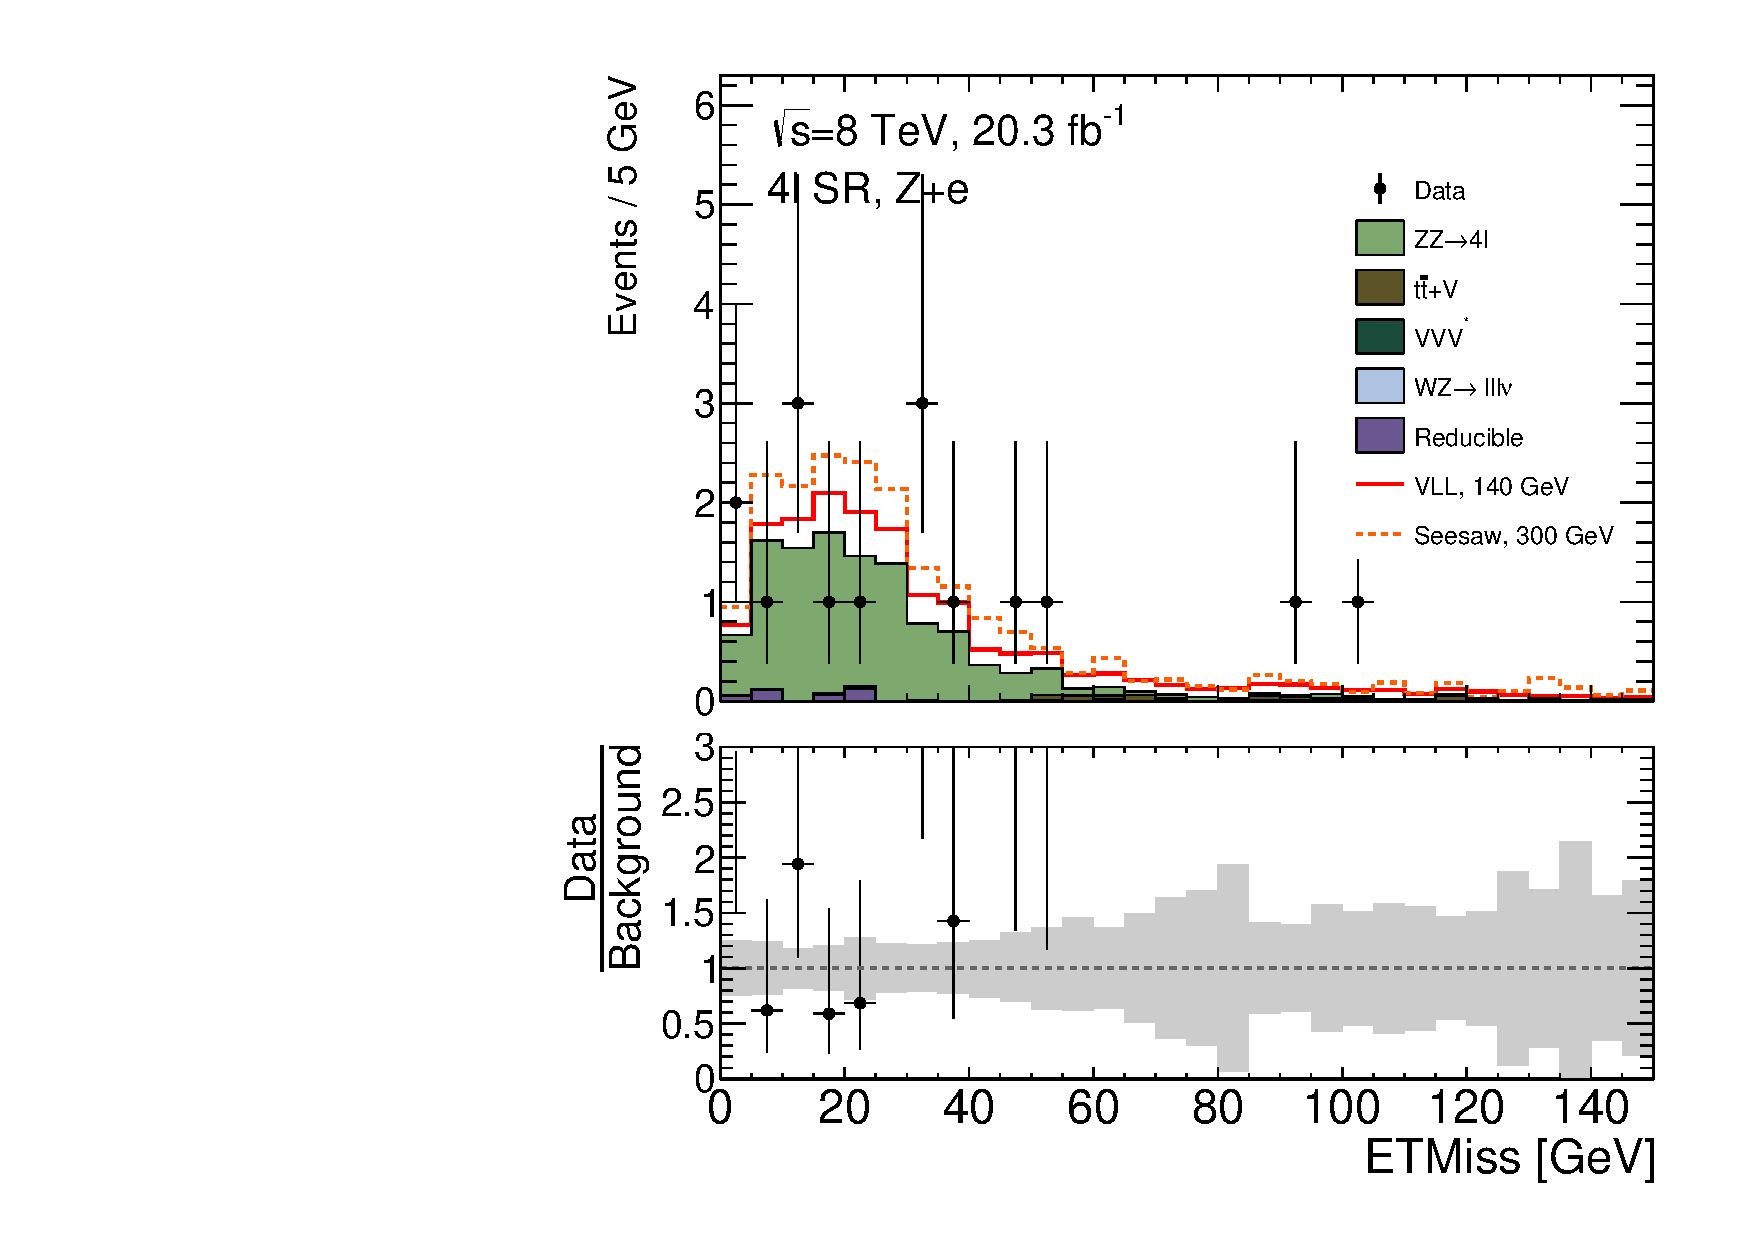
\includegraphics{figures/resonance/c_output_ETMiss_Ze_FourLNoM3L_300GeV}}
  }
  \subfloat[ $Z+\mu$, $4L$ category] {
    \resizebox{0.48\textwidth}{!}{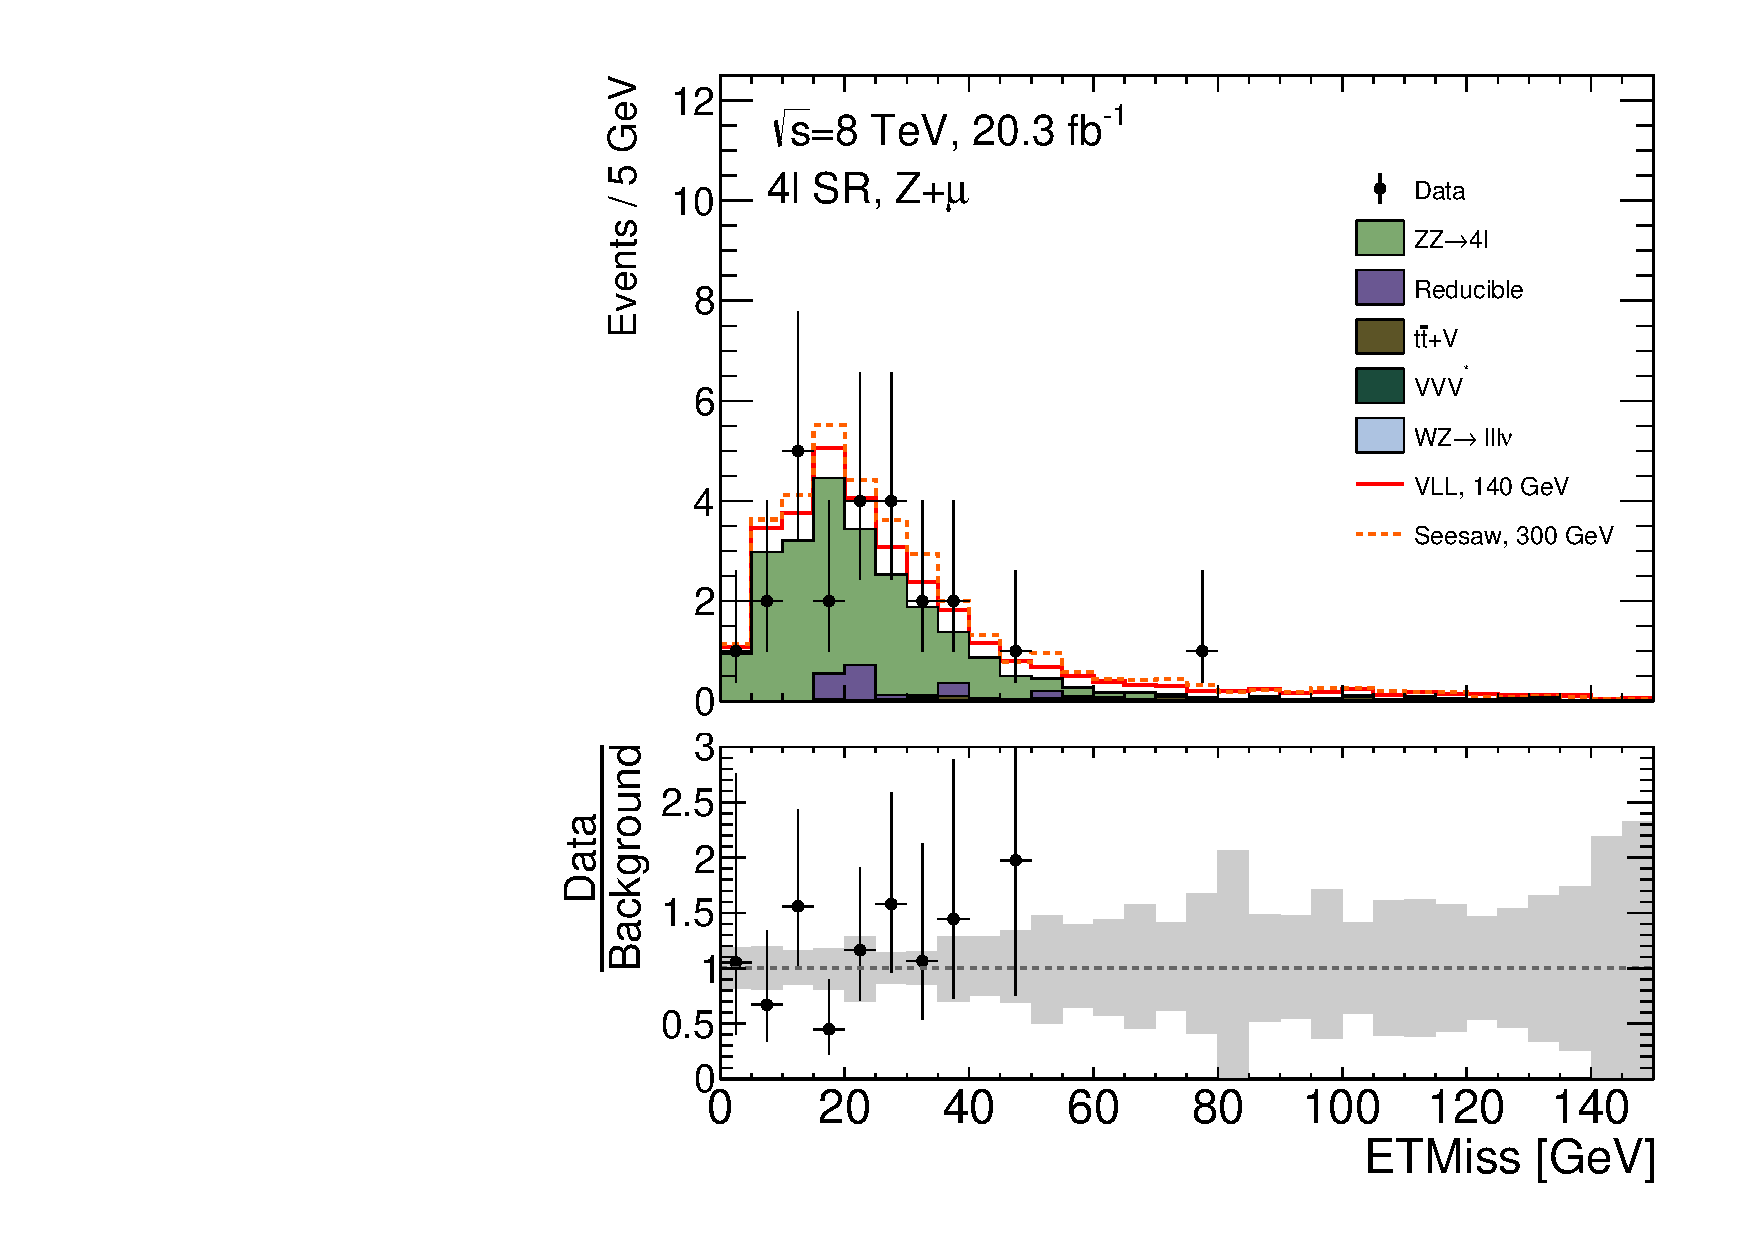
\includegraphics{figures/resonance/c_output_ETMiss_Zmu_FourLNoM3L_300GeV}}
  } \\
  \caption{Missing energy ($\Etmiss$) for $Z+e$ and $Z+\mu$ candidates, for the inclusive and $\fourl$ signal regions.}
  \label{fig:SR-ETMiss-1}
\end{figure}

\clearpage

\begin{figure}[htb]
  \centering
  \subfloat[ $Z+e$, dijet category] {
    \resizebox{0.48\textwidth}{!}{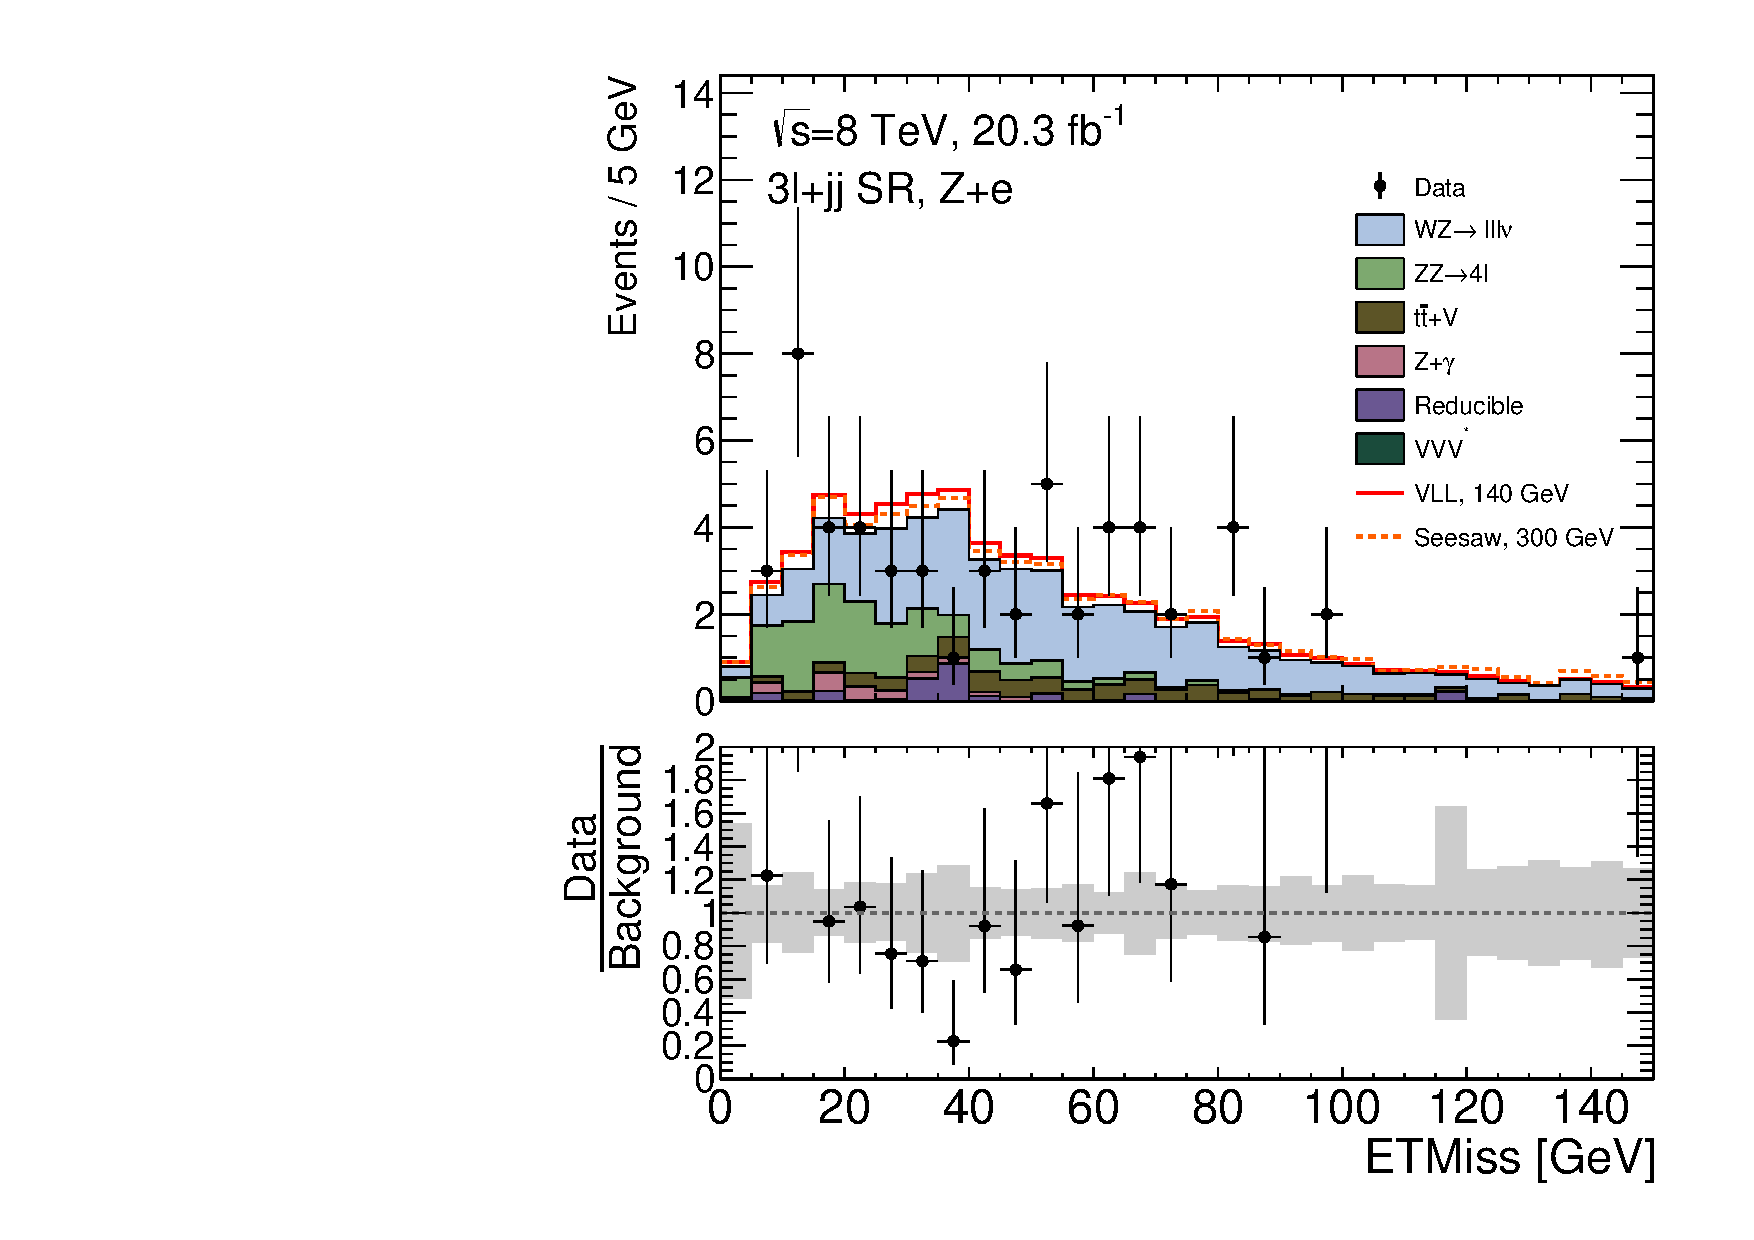
\includegraphics{figures/resonance/c_output_ETMiss_Ze_ThreeLDijetNoM3L_300GeV}}
  }
  \subfloat[ $Z+\mu$, dijet category] {
    \resizebox{0.48\textwidth}{!}{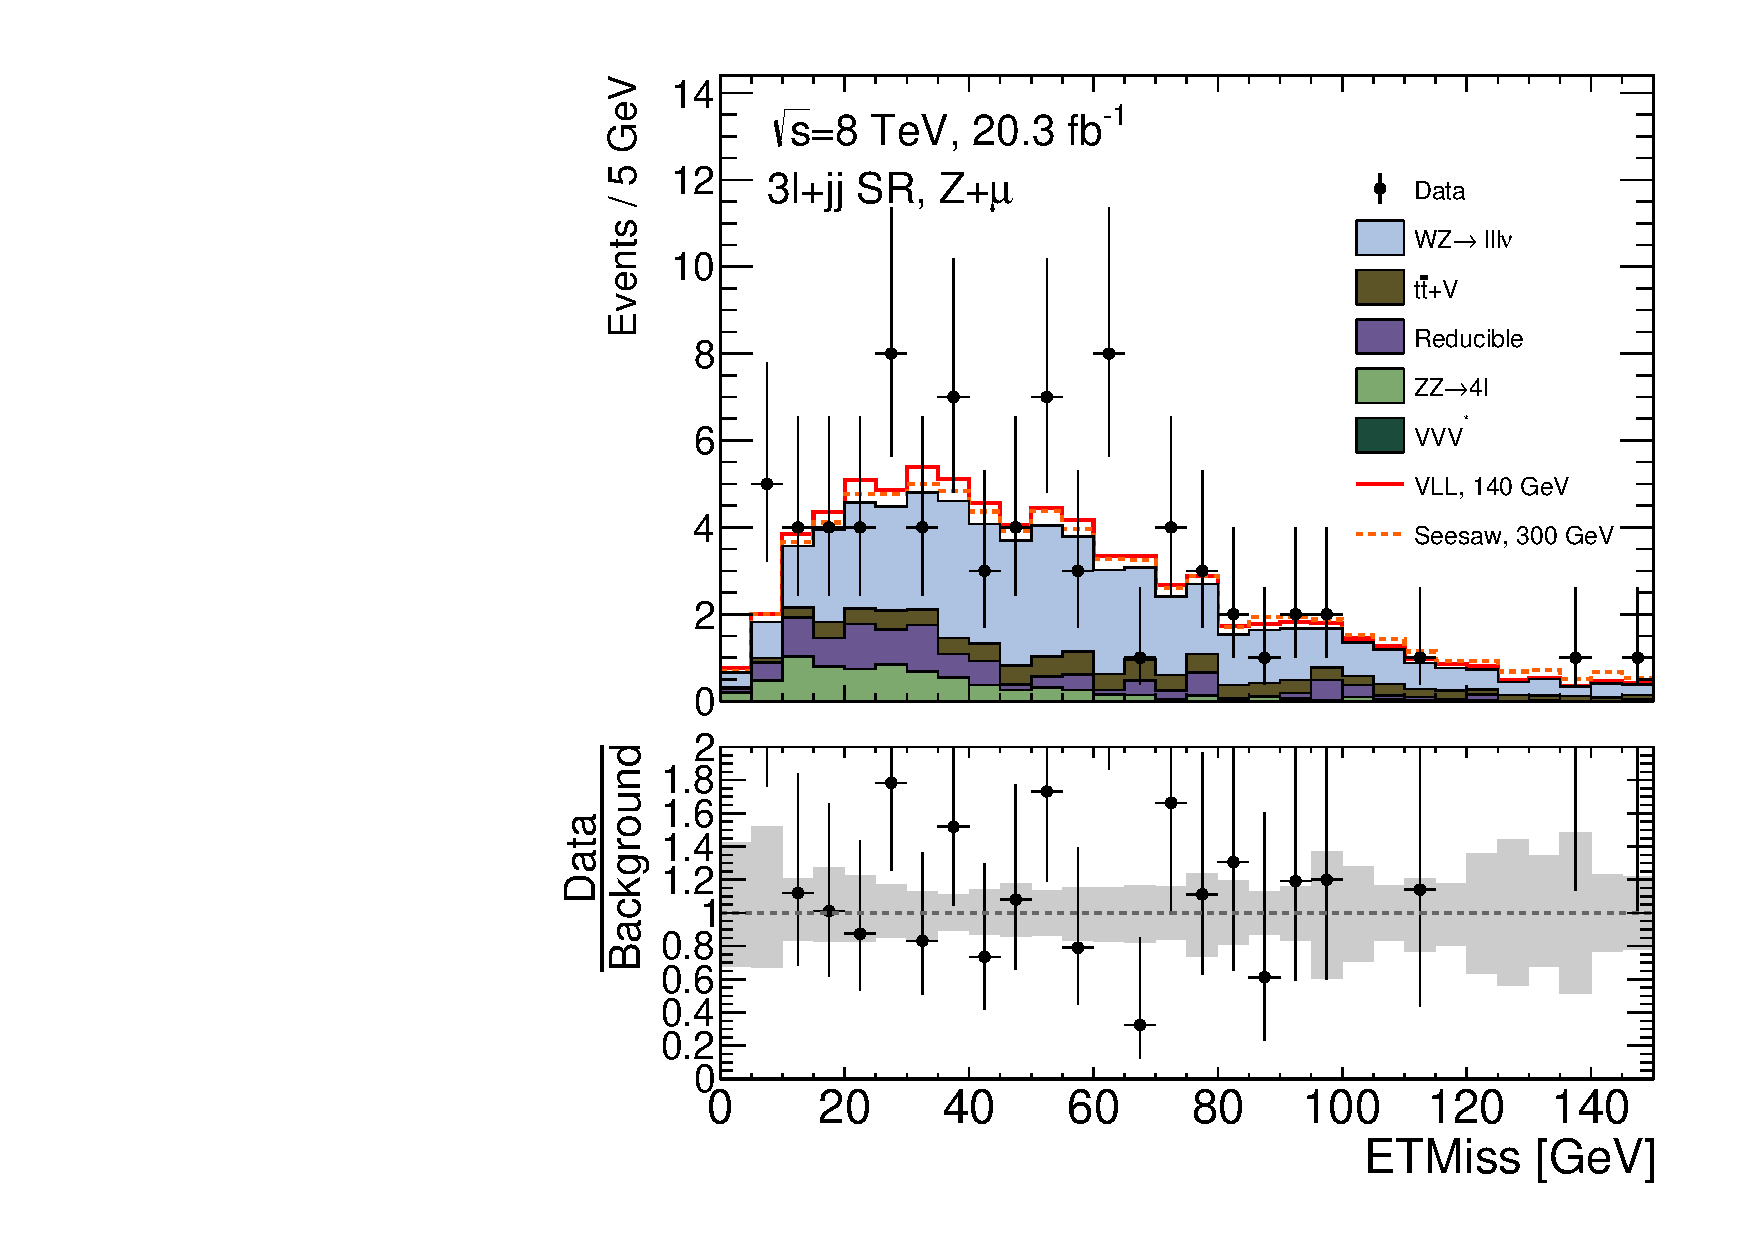
\includegraphics{figures/resonance/c_output_ETMiss_Zmu_ThreeLDijetNoM3L_300GeV}}
  } \\
  \subfloat[ $Z+e$, else category] {
    \resizebox{0.48\textwidth}{!}{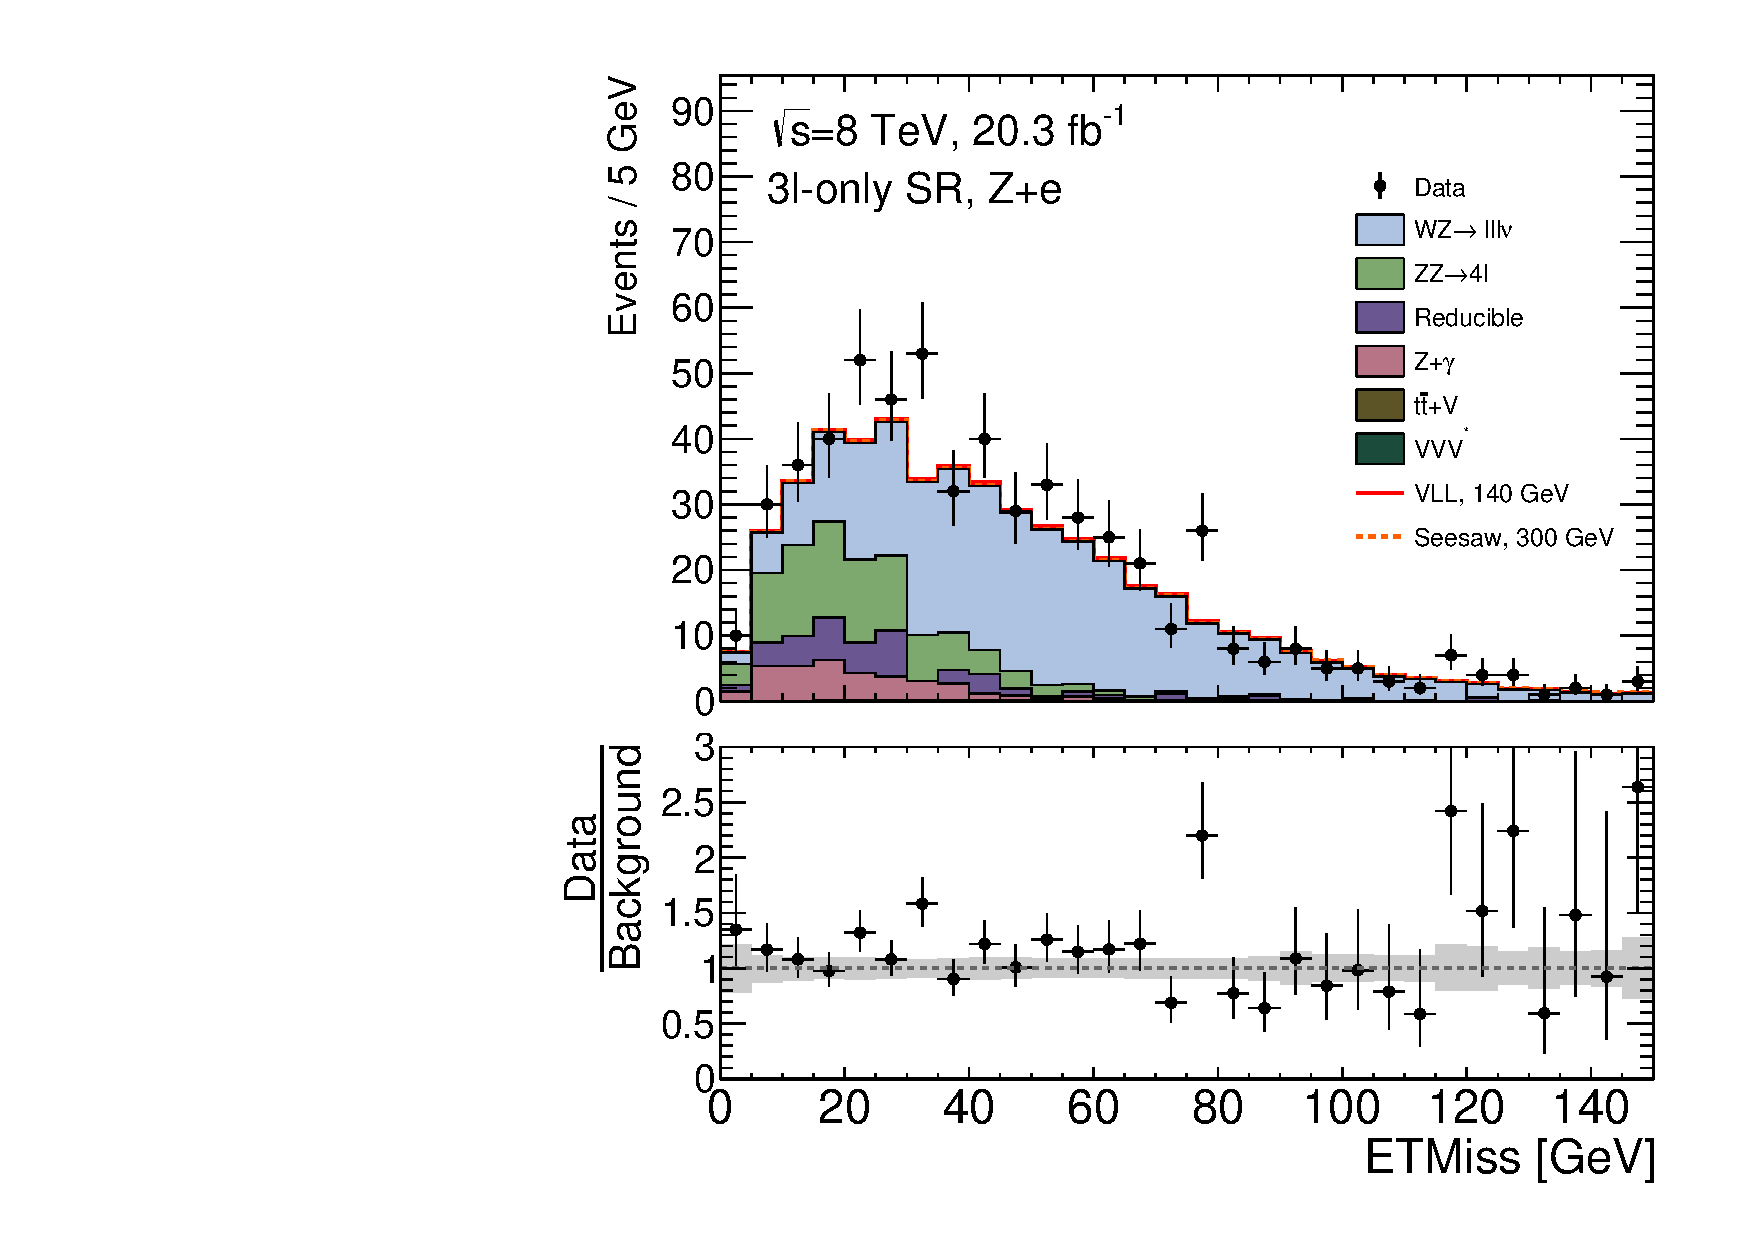
\includegraphics{figures/resonance/c_output_ETMiss_Ze_ElseNoM3L_300GeV}}
  }
  \subfloat[ $Z+\mu$, else category] {
    \resizebox{0.48\textwidth}{!}{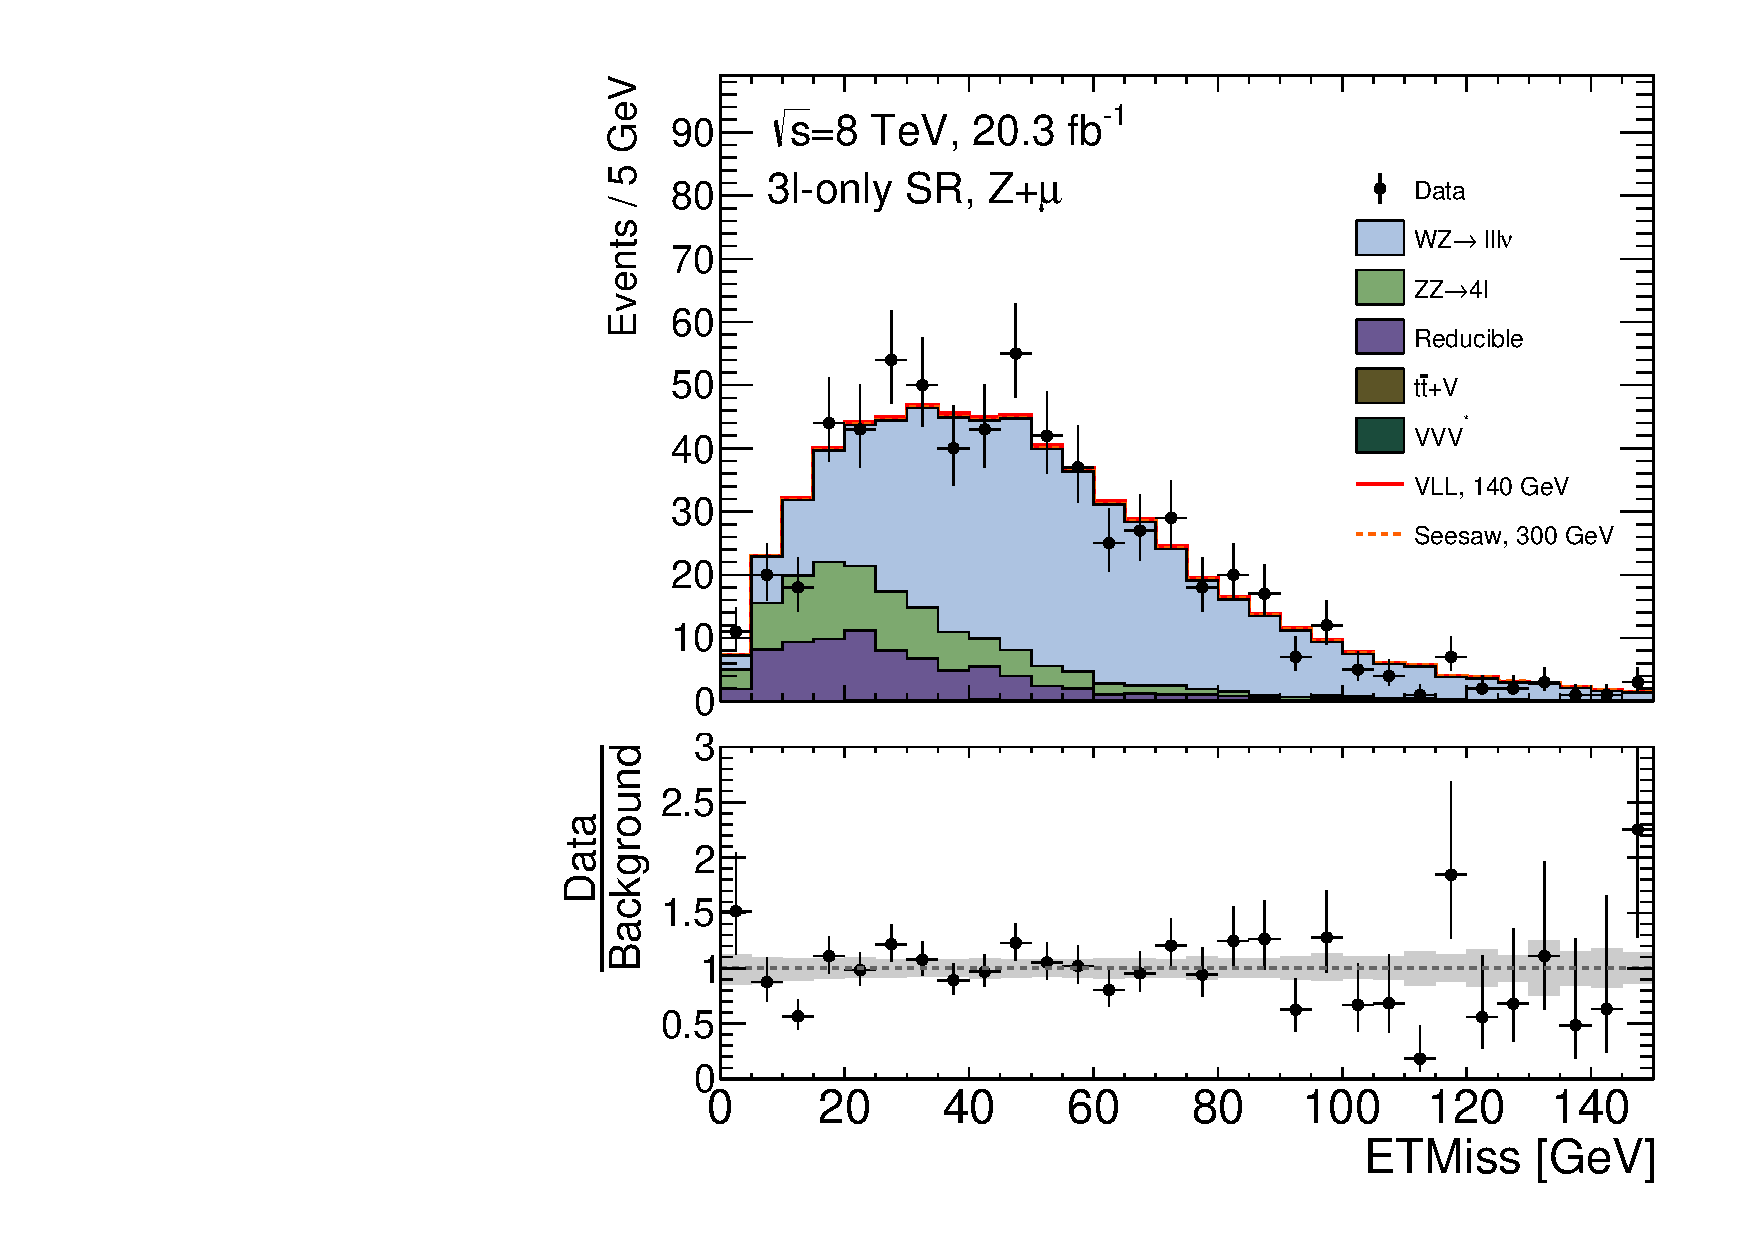
\includegraphics{figures/resonance/c_output_ETMiss_Zmu_ElseNoM3L_300GeV}}
  }
  \caption{Missing energy ($\Etmiss$) for $Z+e$ and $Z+\mu$ candidates, for the $\threeljj$ and $\threelo$ signal regions.}
  \label{fig:SR-ETMiss-2}
\end{figure}

\clearpage

\chapter{Statistical Methods}\label{appx:statistics}
The analyses presented in chapters~\ref{ch:model-independent-trilepton-search} and \ref{ch:trilepton-resonance-search} both employ a modified frequentist approach to the statistical limit setting known as the $CL_s$ method~\cite{cls}. The goal of the method is to compare the data against the signal plus background hypothesis versus the background-ony hypothesis. In the case of searches, the signal plus background hypothesis is assumed to predict an excess of events above the background-only hypothesis. 

The first step is to define a \emph{test statistic}, $\tilde{q}_{\mu}$, which distinguishes a background-like data sample from a signal plus background-like sample. Here $\mu$ is a parameter representing the signal strength; $\mu=1$ corresponds to the signal hypothesis ($S+B$), while $\mu=0$ corresponds to background only ($B$). The test statistic is based on the profile likelihood method. In the cased of binned data, i.e. a histogram with $N$ bins, the likelihood is given by,

\begin{equation}\label{eqn:binned-likelihood}
	\mathcal{L} = \left(\prod_{i=1}^N \frac{\mu s_i + b_i}{n_i!} e^{-(\mu s_i + b_i)}\right) \times \rho(\tilde{\theta}|\theta),
\end{equation}

where $s_i$ and $b_i$ are the expected number of signal and background events in bin $i$ and $n_i$ is the number of observed events in bin $i$. The systematic uncertainties are parametrized by a set of nuisance parameters, $\theta$, with nominal values $\tilde{\theta}$; the $\rho(\tilde{\theta}|\theta)$ are frequentist auxiliary measurement probability distribution functions (pdfs) of the nuisance parameters, which are taken to be Gaussian for most sources of uncertainty considered here. This formalism applies to the model-independent trilepton search, where the signal regions are effectively one-bin histograms. 

In the case of unbinned data, $\{x_i\}_{i\in [1,k]}$, the likelihood is given by,

\begin{equation}\label{eqn:unbinned-likelihood}
	\mathcal{L}=\frac1k \left(\prod_{i=1}^{k} \left(\mu S f_s(x_i) + B f_b(x_i)\right) \times e^{-(\mu S + B)}\right) \times \rho(\tilde{\theta}|\theta),
\end{equation}

where $S$ and $B$ are the total expected number of signal and background events, and $f_s(x_i)$ and $f_b(x_i)$ are the signal and background pdfs for the data $x_i$. This formalism applied to the trilepton resonance search, where the signal and background are parametrized by analytical functions. 

The test statistic is taken to be the negative log likelihood ratio,

\begin{equation}\label{eqn:NLLR}
  \tilde{q}_{\mu} = -2\log \left(\frac{\mathcal{L}(\mathrm{data}|\mu,\,\hat{\theta}_{\mu})}{\mathcal{L}(\mathrm{data}|\hat{\mu},\,\hat{\theta})}\right).
\end{equation}

Greater values correspond to more background-like observations, and lesser values correspond to more signal-like observations. Here, $\hat{\theta}_{\mu}$ is a conditional maximum likelihood estimator (MLE) of the nuisance parameters $\theta$ given the data for fixed $\mu$, and $\hat{\mu}$ and $\hat{theta}$ are global MLEs of the signal strength and nuisance parameters. The value of $\hat{\mu}$ is restricted to be in the range $[0,\,\mu]$; the lower bound enforces the expectation that the signal produces an excess, while the upper bound guarantees a one-sided confidence interval, ensuring that an upwards fluctuation beyond $\mu$ would not count against the signal plus background hypothesis. 

To find the observed limit on $\mu$, pdfs are derived for $\tilde{q}_{\mu}$ under the $S+B$ and $B$ hypotheses ($f(\tilde{q}_{\mu}|\mu,\,\hat{\theta}_{\mu}^{\mathrm{obs}})$ and $f(\tilde{q}_{\mu}|0,\,\hat{\theta}_{0}^{\mathrm{obs}})$) using toy Monte Carlo pseudoexperiments
%\footnote{An \emph{unconditional ensemble} is generated, i.e. the nuisance parameters are randomized about their nominal values, so that the distribution agrees with asymptotic expressions.}
. The nuisance parameters are fixed to the maximum likelihood estimates, $\hat{\theta}_{\mu}^{\mathrm{obs}}$ and $\hat{\theta}_{0}^{\mathrm{obs}}$ for the $S+B$ and $B$ hypotheses, respectively. Example pdfs are shown in figure~\ref{fig:qmu-pdfs}. 

Given an observed test statistic $\tilde{q}_{\mu}^{\mathrm{obs}}$, the pdfs are used to derive $p$-values for the $S+B$ and $B$ hypotheses:

\begin{align}\label{eqn:p-values}
	p_0 &= P(\tilde{q}_{\mu}\leq \tilde{q}_{\mu}^{\mathrm{obs}}|B)=  \int_{\tilde{q}_{\mu}^{\mathrm{obs}}}^{\infty} f(\tilde{q}_{\mu}|0)\,\mathrm{d\tilde{q}_{\mu}} \\
	p_{\mu} &= P(\tilde{q}_{\mu}\geq \tilde{q}_{\mu}^{\mathrm{obs}}|S+B) = \int_{\tilde{q}_{\mu}^{\mathrm{obs}}}^{\infty} f(\tilde{q}_{\mu}|\mu)\,\mathrm{d\tilde{q}_{\mu}}. \\
\end{align}

The $p_0$ value gives the probability of obtaining a test statistic equal to or more signal-like than observed, assuming the background-only hypothesis. Similarly, the $p_{\mu}$ value gives the probability of obtaining a test statistic equal to or more background-like than observed, assuming the signal plus background hypothesis. 

Finally, the $\cls$ method defines the criterion used to exclude a model. The $\cls$ value is constructed to avoid the problem of excluding models to which the experiment has little sensitivity; for example, a large downward fluctuation can result in the $p_{\mu}\equiv \clsb$ value excluding $\mu=0$, even if the experiment has no sensitivity to the signal. A model with signal strength $\mu$ is considered excluded at confidence level $1-\alpha$ if:

\begin{equation}\label{eqn:cls}
	\cls \equiv \frac{p_{\mu}}{1-p_0} < \alpha.
\end{equation}

Note that the $\cls$ value is not itself a $p$-value, but satisfies $\cls > p_{\mu}\equiv \clsb$, and hence is more conservative than $\clsb$. The 95\% confidence level observed exclusion is determined by solving for the $\mu$ value which yields $\cls=0.05$.



\printbibliography

\end{appendices}

